%% The openany option is here just to remove the blank pages before a new chapter
\documentclass{book}
\usepackage{graphicx}
\usepackage{tcolorbox}
\usepackage{textgreek,url,fancyvrb}
\usepackage{soul}
\usepackage[caption=false]{subfig}
\usepackage[top=1in, bottom=1in, left=1 in, right= 1 in]{geometry}
\usepackage{float}
\usepackage{enumitem}
\usepackage{listings}
\usepackage{csquotes}
\usepackage{url}
\usepackage{todonotes}
\usepackage{enumitem}
\usepackage{hyperref}

\renewcommand{\familydefault}{\sfdefault}

\hypersetup{linkcolor=blue, linkbordercolor=0 0 1, colorlinks=true}

\makeatletter
 \def\@textbottom{\vskip \z@ \@plus 1pt}
 \let\@texttop\relax
\makeatother


\setitemize{noitemsep,topsep=1pt,parsep=1pt,partopsep=0pt}
\lstset{
language=C,
numberstyle=\footnotesize,
basicstyle=\ttfamily\footnotesize,
stepnumber=1,
breaklines=true,
showspaces=false,           % Leerzeichen anzeigen ?
showtabs=false,             % Tabs anzeigen ?
frame=L
 }

\newcommand{\specialcell}[2][l]{%
	\begin{tabular}[#1]{@{}l@{}}#2\end{tabular}}


\begin{document}

\title{{ ~\\~\\~\\~\\~\\ Data Structures in C \\\Large ~\\Lecture Notes for  CIS*2520 \\~\\University of Guelph\\~\\~\\~\\~\\}}
\author{Judi McCuaig }
\maketitle

\Huge 
Foreward
\\ \\ \\
\normalsize
This document was originally written as supplement to the slides and lectures for CIS*2520.  Recently(early 2017) it has been revised to serve as the main reference document for a distance education version of CIS*2520.   Students using this material are assumed to have  a background in programming in C.   

Special thanks to David McCaughan, Pascal Matsakis and Xining Li for sharing  slides and presentations from their offerings CIS*2520.  D. McCaughan's materials influenced the overall design of the course materials significantly.   Dr. Matsakis and and Dr. Li's work helped greatly to  improve the material on computational complexity,  heaps, and priority queues.


This work is licensed under a Creative Commons Attribution-NonCommercial-ShareAlike 4.0 International License.


\tableofcontents


\mainmatter




%
\chapter{Introduction}

\textbf{Welcome to CIS 2520!}

A data structures course is often the first course in a series of courses on software design.  
During this class we will examine a variety of abstract data types and how they can be used to improve the quality of the software you develop. This e-text contains all the notes provided as part of the course website as well as more detailed material for in-depth study.  
 
The examples will be given in pseudo code that could be used as the outline for a program in nearly any programming language, or in c.   The pseudocode format is as follows:  

\begin{itemize}
\item function and procedures are defined with a name that begins with a lower case 
\item parameters are included as types only 
\item if there is a return value,   it appears at the end of the function definition after a colon
\item no ending punctuation is used for lines
\item indentation is used rather than parentheses  
\end{itemize} 
For example a pseudocode function could be defined as :    

\begin{lstlisting}
calculateComplicateValue(int, String): int
\end{lstlisting}
 If the same function were actually written in a C header file it would look something like this:  
 \begin{lstlisting}
 int calculateComplicateValue(int intVal, char * stringVal);
 \end{lstlisting} 
\section{Why Software Design}

Most software is not developed by a single person and most of it takes months or even years to complete and test.   Most software development involves multiple people who subdivide the problem into chunks and then collaborate to make the entire program work.
 
The process of identifying suitable chunks is the essence of software engineering.   When the chunks are defined so that a single chunk can be reused in more than one software project, the company benefits because it only pays once for the development of something than can be used more than once.  Good software engineering   practices save time (on the part of the developer) and money (on the part of the employer or funding organization).


In future courses, you will spend time learning about a variety of formal approaches to software development.    Each formal approach represents one way to try to meet the objectives of modularity, maintainability, reuse, low coupling, high cohesion when creating software with medium-large teams. The effectiveness of each formal approach depends on the type of software being developed, on the development environment and context, and on the personalities of the development team.


\section{Software Development- CIS 2520 Style}

Clean, crisp coding habits are developed over time, not learned all at once.   And, like any good (or bad) habit, if you don’t practice, you’ll lose the habit.   You are expected to follow good coding practices for all of your homework in this class.     Consistency is the key to writing readable code.   For all work for 2520, you are expected to follow the following minimum set of conventions.

\begin{itemize}

\item Use a consistent naming convention for all variable names.  Variable names must be meaningful with single-character names used only for counters.
\item The names for types (including abstract data types) must be obviously different from the names for variables.  For example, you could capitalize the first letter of the names of a type.
\item Use spaces for indentation- do not use tabs
\item Use .h files to declare functions and types and put implementation in .c files.  You may, or may not, need a .h file for the file containing main.   Use include-guards in your .h files.
\item Organize your .h files and .c files so that functions are in the same order in both files.  Use blank lines to create groups of code.   
\item Doxygen style comments go in the .h file for every function (as a minimum)  
\item Every source code  or .h file begins with a doxygen comment  that indicates author, purpose of code, and last modification date.
\item Compile your code with -Wall and -g flags.  You may use -ansi, -std=c99 or -std=c11
\end{itemize}


You must submit modular code for your homework solutions.  This means you must break programs into separate files.   
\begin{itemize}
\item Use makefiles to automate the build process so that you can divide your code into as many modules as necessary.    
\item Each file in your project should contain a single module that goes together in some way (i.e. a module for reading in files,  a module for calculating things,  a module for list operations).
\item Your programs must be organized in a file structure that contains src/  bin/ include/  assets/  and docs/  folders and your makefile must make use of that file structure.   src/ is for source code,  include/ is for .h files,   docs/ is for doxygen documentation,  and assets is for testing files, data files, etc.   The README goes in the root folder of an assignment, not in the sub folders.
\item The README file should be based on the template shown below.  Read assignment specifications carefully as there may be additional information  expected in assignment-specific README files.
\end{itemize}

\clearpage
\textbf{Sample README format}
\begin{verbatim}
****************************************************
Your name		        Your student number
The class name		The assignment name/number
The date                          Your uoguelph email address
****************************************************

************
Compilation
************
in this space write down how to compile your program
include descriptions of all the targets in your makefile

***********************
Running the program(s)
***********************
in this space describe how to run your program
please don't run programs out of your makefile
include a description of any command line arguments

*****************
Known Limitations
*****************
in this space write down any of the limitations (unfinished bits) that your program has
\end{verbatim}

\section{Test driven development }

 It is not enough to simply have a program that runs,   it must run properly and produce correct results for all allowable inputs.  One way to do that is to set up the testing program as the first thing you do, and then to test early and to test often.   
 
 Instead of writing the entire solution to your homework, create a skeleton that that is just the framework of your program but no functionality.  The skeleton should have all the files, all the functions  definitions,  all the structures and types, but none of the actual functionality.  The values returned by functions and any actual data processing is completely hard coded.    This is called writing a \textbf{stub} for a function.  
When you have created a complete skeleton for your program, you can then add functionality to one function or procedure at a time and test just that function.
 
Use a driver or test harness to test your code modules.  Write the test harness as a series of function calls in main, using hard coded data for which you know the return value.  Add checks and comparisons to determine if value returned by your function is the expected value.  Once your software can pass all of the tests in your test harness, then it is time to write a new 'main' that is the actual application.
 
Create test data that cover all the different types of possible data.   Test for edge cases (zero or null values,   really big values, too many values, etc).   Test each function with  values having different attributes so that you can show you have thoroughly tested the different parts of your software.

For example,  below you can find  the skeleton code for a singly linked list of string data.  You have likely worked with linked lists in a previous course.  The code given contains no functionality, but it will compile and run with a test harness.    Note:  This skeleton code should not be your starting point for the first lab as it does not meet the requirements for the first lab.   The skeleton code also gives you an example of doxygen-styled comments, which are required for this course and of how to use include guards in your .h file.


The .h file contains the function prototypes and the struct definitions and  the comments for each function.
\begin{lstlisting}
/**
 * @file linkedList.h
 * @author Judi McCuaig
 * @date January 2017
 * @brief API for a singly linked list
 */
#ifndef _JRM_LLIST
#define _JRM_LLIST
struct listNode {
    char * nodeValue;
    struct listNode * next;
};
typedef struct listNode node;

/** Creates a list and returns a pointer
*@return pointer to the list head
**/
node * createList ();
/** Destroys the list and frees all the allocated memory
*@param pointer to the head of the list
**/
void destroyList(node * head);
/** Adds an element to the head of the list
*@param pointer to the head of the list
*@param pointer to the string that will be stored in the list
**/
void addFront (node * head, char * data);
/** Removes a specific element from the list and frees the memory for that element
*@return 0 if the removal is successful, -1 on error
*@param pointer to the head of the list
*@param pointer to the string that will be removed from the list
**/
int removeFromList(node * head, char * data);
/** Prints the list in head-to-tail order
*@param pointer to the head of the list
**/
void printList(node * head);
/** Frees the memory allocated for a list node
*@param pointer to the node to be freed
**/
void freeElement (node * element);
/** Creates a list node with the data provided in the parameter
*@return pointer to the new node
*@param pointer to the data to be stored in the node
**/
node * initElement(char * data);

#endif
\end{lstlisting}

\clearpage
The source code (.c) file contains the implementation for the functions.
\begin{lstlisting}
/**
 * @file linkedList.c
 * @author Judi McCuaig
 * @date January 2017
 * @brief skeleton code for a singly linked list
 */
#include "linkedList.h"

node * createList ()
{
       return (NULL);
}

void destroyList(node * head)
{    
}

void addFront (node * head, char * data)
{    
}


int removeFromList(node * head, char * data)
{
   return(0); 
}


void printList(node * head)
{
    printf("\n");
}


void freeElement(node * element)
{
}

node * initElement(char * data)
{
}
\end{lstlisting}

\section{Extending Activities}

\begin{itemize}

\item The internet has many high quality resources about software engineering and software design.  Build yourself a list of resources for information.  Look for podcasts, videos, websites, or newsgroups that can help you arrive at definitions for each of the following:   Modularity,   Reuse, Maintainability,   Coupling,   Cohesion.     You may use Wikipedia, but try to find other resources as well.



\item There are many different processes for developing software.  A common (and old) process is called the Waterfall cycle and involves rigidly dividing the process into definition, design, development and testing segments.  Each segment is completed before the next segment is started.  Other processes are more fluid, moving between design and development as new requirements are noted.
 It is very difficult to use a formal software development process as part of coursework because most of the design process is done for you when the assignment specification is done.   Still, it is possible to use portions of specific approaches.   The lab activities for 2520 are based on a modified Test-Driven development cycle.    Use internet resources to inform yourself about Test-Driven development.  Make list of the changes you will need to make to your own development habits in order to be successful in a test-driven process.
\end{itemize}

\chapter{Abstraction}

\section{Introduction}
While computer hardware has changed significantly over the past several decades, the way in which we communicate with computers has not changed very much at all. The basic instructions and building blocks used in a computer program are the same now as they were when computers were constructed from mechanical parts.
At the machine level, a program is a set of instructions composed of arithmetic and logic, and the data used and the instructions of the program are all represented as binary numbers. Most programmers rarely, if ever, interact directly with the binary machine code when creating computer programs. Instead a programmer uses a higher level language, an abstraction, that provides single instructions that represent several machine code steps.
For example, in machine code, the instruction to add two numbers might look something like this:

00001001 0000000001100011 000000000110010

where the first number represents the instruction for add, and the second number is the memory location of one value to be added and the third number is the memory location of the second value to be added. This example code does not include putting the result of the addition anywhere useful for the programmer- that is a second step.
Abstracted programming languages greatly improved the productivity and reliability of the programs written. Such languages are often called 'high level' languages. C, Pascal, Cobol, LISP, and Fortran are among the first high level languages developed. Each of these languages was specialized somewhat to create usable abstractions for operations that were common to a particular class of computer programs. Cobol has specialized operations for business and was created so that even non-programmers could understand the code. Fortran is specialized for mathematics, and LISP is specialized for artificial intelligence programming.
In more recent years, even higher level languages have been abstracted from the early languages



\section{Real World Abstraction}
Abstraction is a tool that we use to navigate the world around us. A map is an example of an abstraction. A map contains information about a real space, but it only contains the information that is relevant to moving around in that space. Maps do not contain ALL the details about a space because that would make the map unreadable.

An abstraction is a representation of something that shows only the details that are essential for the task at hand, and ignores the other details. Think again about the map example. A topographical map has different details than a street map. A map that outlines points of interest for a nature walk would have different details than a map constructed for a geological survey.

Abstraction is used to make devices usable in situations where it is unnecessary to understand all the details in order to use something. The modern car is usable by persons who have little or no mechanical aptitude. The details that the driver sees are relevant for safe driving, and all the details about how the car operates have been hidden from the driver.

The utility supply to your house is an abstracted interface. You can use electrical power in your house without needing any details about how that power is generated, or how your house is wired. You don't even need to understand how electricity works.
A good abstraction is one that simplifies the use of something, but that still permits use in many general situations. Sometimes abstraction is unnecessary.


Consider the kitchen can opener. Many different kinds of can openers can be purchased, with a widely varying level of abstraction. Each higher level abstraction hides a few more details about how the can opener works. All can openers eventually open the can, the difference is in the amount of effort and understanding required of the operator.

\begin{figure}[H]
\centering
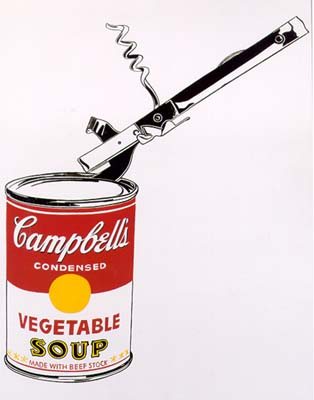
\includegraphics[width=0.3\textwidth]{pictures/Campbell_s_Soup_with_Can_Opener.jpg}
\label{fig:canOpener1}
\end{figure}

This example makes it very clear that the can is opened by wiggling a sharp knife up and down through the metal.

\begin{figure}[H]
\centering
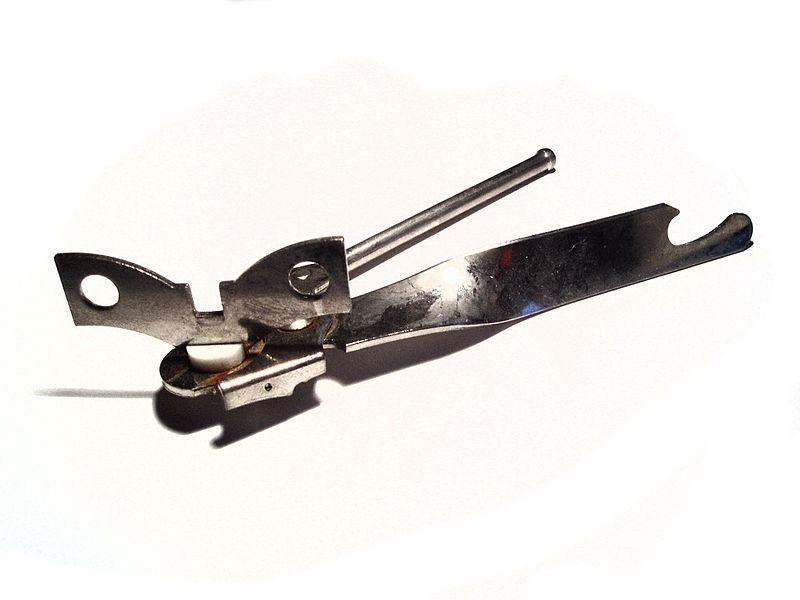
\includegraphics[width=0.3\textwidth]{pictures/800px-Can_Opener.jpg}
\label{fig:canOpener2}
\end{figure}

This version has a circular knife, which hides the sawing motion with a crank, but the pressure required to operate it makes it very clear that a knife is still cutting through metal.

\begin{figure}[H]
\centering
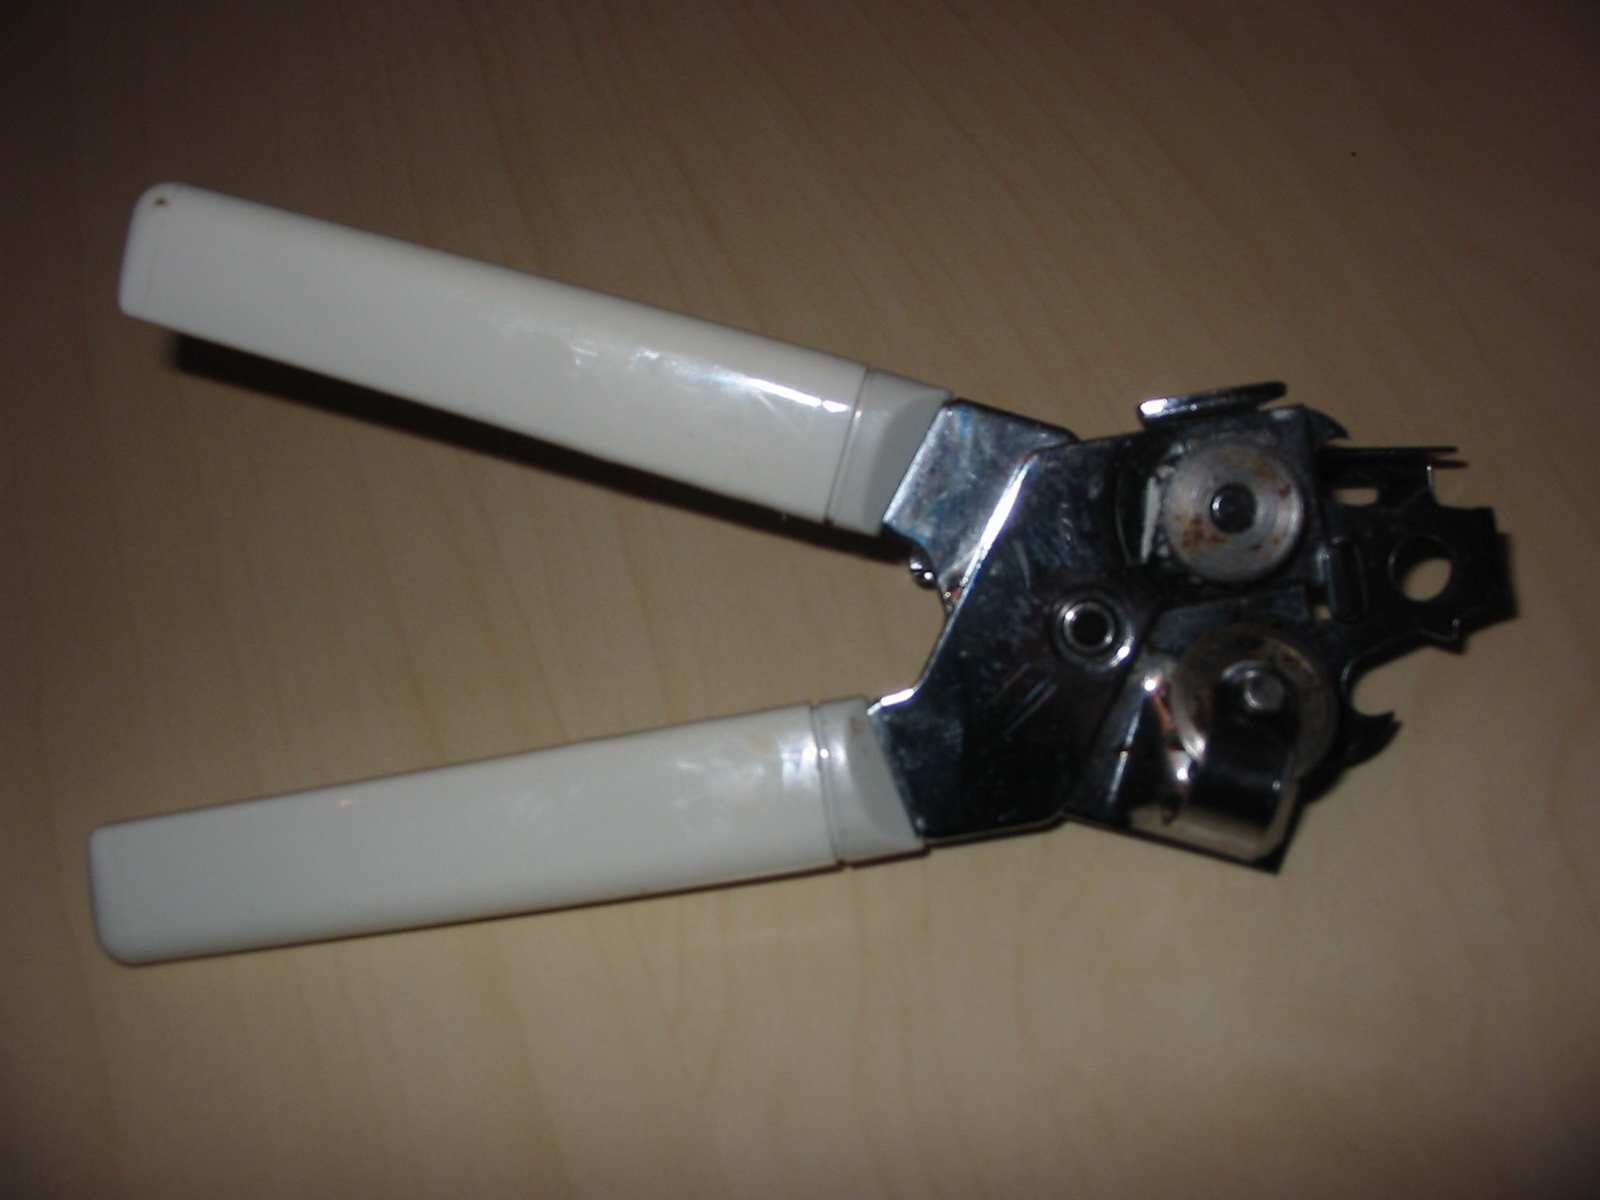
\includegraphics[width=0.3\textwidth]{pictures/Can_opener.JPG}
\label{fig:canOpener3}
\end{figure}

\subsection{Implementation}

An abstraction is really just a design until it is implemented in some way. It is possible to design an abstraction, and then have several different implementations, all with different strengths and weaknesses.

Suppose that you had been tasked to create a device to cook an egg without requiring the cook to crack the egg. One possible implementation for such an egg-cooking device is this

\begin{figure}[H]
\centering
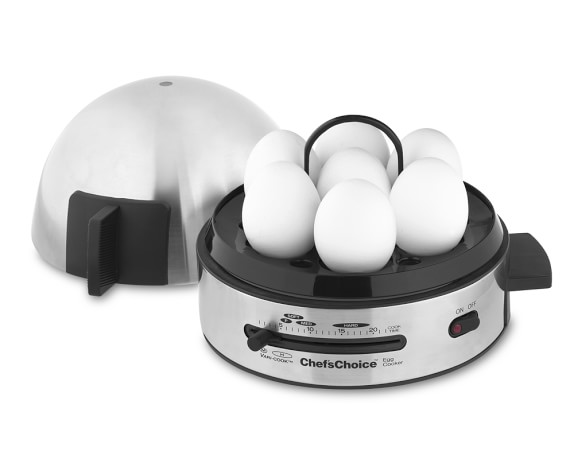
\includegraphics[width=0.3\textwidth]{pictures/chefschoice-electric-egg-cooker-c.jpg}
\label{fig:eggCooker1}
\end{figure}

Another possible implementation could look like this

\begin{figure}[H]
\centering
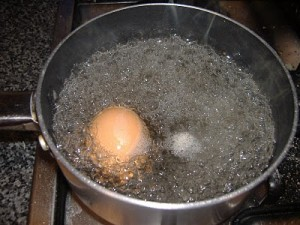
\includegraphics[width=0.3\textwidth]{pictures/boiled-egg-300x225.jpg}
\label{fig:eggCooker2}
\end{figure}


Another implementation can be found here:  \url{http://www.youtube.com/watch?v=XRb82E4_b38}

While these implementations accomplish the task, they are not equal in terms of cost to construct, maintainability, likelihood of breakdown, etc.



\section{Abstraction in Software Design}

The image below illustrates the different levels of abstraction required to create a computer program for managing a sports complex. The highest level of abstraction, the application level, maps the ideas and concepts of the real world to the specification of the program operation.

\begin{figure}[H]
\centering
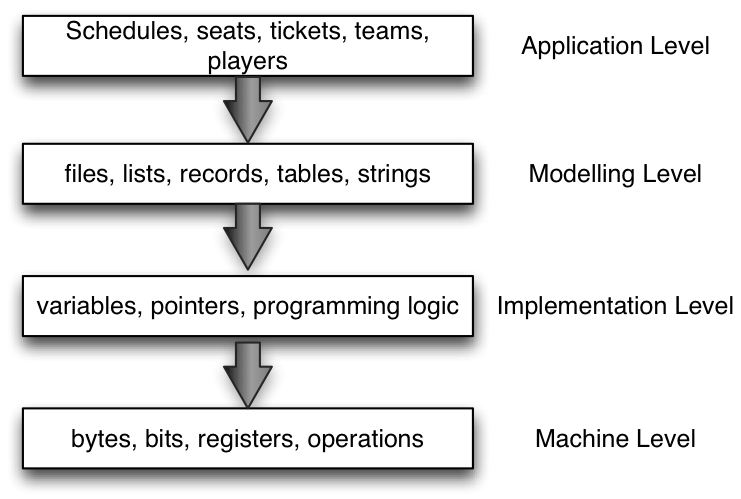
\includegraphics{pictures/abstraction01.png}
\label{fig:sportsComplex}
\end{figure}

The second level, the modeling level, maps the objects and entities discovered in the first level to models that can be used to represent the entities in the software. The third level of abstraction creates the actual implementation of those models and the last level is the responsibility of the compiler.

\textbf{In computing, an abstraction lets you understand 'what' can be accomplished without requiring that you know the details of 'how' the thing is accomplished.}

The reason we use abstractions in programming is really for economics. It is more time-efficient for programmers to reuse previously developed (and debugged) libraries than it is for them to program everything in binary. It is also more cost-efficient because the reusable library only needs to be debugged once, and then used many times. This is in contrast to building from scratch each time, which incurs the same debugging requirements for every development effort.

Programming languages, file system libraries, input-output libraries, and string libraries are all examples of abstractions that programmers use every day. Abstract data types 
are another kind of abstraction that programmers use.

Learning how to design a program in layers, and how to work at an appropriate level of abstraction for each layer is a crucial skill for software developers. Most developers are only concerned with the first three levels of abstraction (application, modeling, and implementation), and must learn how to design applications within those layers.

When you are writing software, you must first ensure that you understand the problem. Make sure you know what the software is supposed to do, and that you understand all the conditions surrounding its operation.

Your first task as a software developer is to decompose the problem into application-level constructs. Identify the main ideas in the software problem (like teams and schedules). These are the core 'things' that the software must create, but they are not things that the computer programming language knows anything about.

The second task is to identify a suitable model for each of the things you find in the first step. For example, you might decide that the best way to represent the teams is as a list, but that the best way to represent the ticket line is by using a queue.


In many cases, the developer can use third party libraries as the implementation layer for the models. Thoroughly debugged modules of abstract data types are available for nearly every programming language.
However, in this class you will be asked to create those modules . By the end of the course, you should have your own, thoroughly debugged, library of Abstract Data Types that you can reuse whenever you wish.

\subsection{Abstract Data Types}

Remember that specification (i.e. "what") and implementation (i.e. "how") are two separate things.
For example, if you are writing functions  in your code, the specification is the function header + pre/post conditions and the implementation is the local variables + body of subroutine.

When you are writing abstract data types, the specification is the definition of data type + operations defined on that type. The implementation is the program needed to effect those operations. In C the specification is usually a header file containing type and function declarations together with a .c file in which they are implemented.

Abstract data types are organized into modules. Each module contains the variable definitions (structures) and operations required to meet the specification of the ADT.

The module exports a 'type', such as list or tree or stack that a programmer can use to declare variables. The variables can then be manipulated using the operations defined within the ADT.

The most important part of this process is that the user of the variable types only needs to know WHAT is possible, but has no need to know HOW it is implemented. The type is abstract from the point of view of the user.

An abstract data type is usually provided to the developer in the form of a library or module.

Some operations are common to most ADT specifications. In particular, pretty much all ADT modules need to provide mechanisms for the following operations:
\begin{itemize}
\item Creating the ADT (initialization of internal variables/allocation of dynamic structures)
\item Destroying the ADT (management of de-allocation of dynamic resources)
\item Adding data to the ADT
\item Removing data from the ADT
\item Getting the value of data in the ADT
\end{itemize}
The details of how those operations behave vary in the different kinds of ADTs, but the core purpose of the operation remains constant.

\subsection{Worked Example: The Fraction ADT}

Suppose you were writing a program that required a representation of fractions. It is not always sufficient to convert  fractions to decimals, sometimes fractions need to stay as fractions. A fraction ADT that allowed the programmer to declare a variable of type fraction would be extremely useful.

First, we need a definition of what a fraction is. 
Fraction: A fraction is a number a/b where a,b are integers, b is non-zero.

\subsubsection{Operations}

The first step in designing an ADT is to imagine what operations are required. In addition to the core operations of create, insert, read, destroy the fraction ADT will need:

\begin{itemize}
\item add (subtraction is just adding with negative numbers)
\item multiply (really just repeated adding, but would be nice to have it as a separate operation)
\end{itemize}

\begin{lstlisting}
ADT specification for Fraction

create_fraction(numerator, denominator): Fraction
    preconditions: none
    postconditions: a fraction is created with the appropriate numerator 
                    and denominator
get_numerator(Fraction): number
    preconditions: an initialized Fraction is given as the parameter
    postconditions: none
get_denominator(Fraction): number
    preconditions: an initialized Fraction is given as the parameter
    postconditions: none
destroy_fraction(Fraction)
    preconditons: the parameter Fraction is initialized
    postconditions: the fraction is destroyed and memory released if necessary
add(Fraction, Fraction): Fraction
    preconditions: two initialized fractions are passed in as parameters
    postconditions: the two fractions are added together and the result is 
                    placed in a new Fraction variable that is returned to the 
                    calling procedure
\end{lstlisting}

The ADT could have many other operations as well.   For example, it could have a function to display/print a fraction or the ability to create a fraction  type from a string representation of the fraction (i.e. "one half" or "three fifths").

\subsubsection{Example Code}

Here's an example of what some of the fraction code might look like in C.  First, the .h file contains the definition of the struct as well as the prototypes for the functions that operate on that struct.

\begin{lstlisting}

/**
 * @file fraction.h
 * @author Judi McCuaig
 * @date January 2017
 * @brief API for a fraction ADT
 */
#ifndef _JRM_FRACTION
#define _JRM_FRACTION

fraction.h

typedef struct {
  int integer;
  int numerator;
  int denominator;
} Fraction;

/** Creates a fraction from an integer numerator and denominator
*@return NULL if the creation is unsuccessful
*@param integer value for the numerator
*@param integer value for the denominator
**/
Fraction * create_fraction(int numer, int denom);

/** Adds two fractions and returns a new fraction that is the result of the addition
*@return NULL if the addition is unsuccessful
*@param Pointer the first Fraction operand
*@param Pointer to the second Fraction operand
**/
Fraction * add ( Fraction *fractOne, Fraction *fractTwo );

#endif

\end{lstlisting}

The .c file doesn't need to redefine the struct because the .h file is included.  The .c file is used to flesh out the implementation of the functions.

\begin{lstlisting}
/**
 * @file fraction.c
 * @author Judi McCuaig
 * @date January 2017
 * @brief implementation of fraction ADT
 */
#include "fraction.h"

Fraction * create_fraction(int numer, int denom){
  Fraction * temp = malloc(sizeof(Fraction)*1);
  temp->numerator = numer;
  temp->denominator = denom;
  return(temp)
}

Fraction * add ( Fraction *fractOne, Fraction *fractTwo ){
  Fraction result= malloc(sizeof(Fraction)*1);
  int largeCommonDenominator;
  int part1, part2, numeratorResult;
  hcd = fractOne->denominator * fractTwo->denominator;
  part1 = fractTwo->denominator * fractOne->numerator;
  part2 = fractOne->denominator * fractTwo->numerator;
  numeratorResult = part1 + part2;
  result->numerator = numeratorResult;
  result->denominator = largeCommonDenominator;
  return result;
}
\end{lstlisting}

The fraction ADT can be used by simply including the .h file in the c program that needs the ADT and then compiling the fraction.c program in with the application.c program.

\begin{lstlisting}
/**
 * @file application.c
 * @author Judi McCuaig
 * @date January 2017
 * @brief use of Fraction ADT
 */
#include "fraction.h"

int main(void){
  Fraction * myFraction = create_fraction(1,2);
  Fraction * myOtherFraction = create_fraction(3,4);
  Fraction * theAnswer = add(myFraction, myOtherFraction);
}

\end{lstlisting}


\section{Information Hiding (Encapsulation)}
Information Hiding is one way to achieve abstraction.  The details of the library implementation are hidden by providing functions to perform operations on the data structure instead of allowing programmers to work directly with the attributes of the data structure. The user of the ADT must use ONLY the interface (the available operations) of the ADT and must resist the temptation to go 'under the hood' and use the component parts.

Information Hiding is also called encapsulation.  Encapsulation helps to prevent errors when a library of functions is updated. For example, suppose you were using a String ADT that provides a stringLength(String) operation to return the length of the string. Suppose further that you knew that the length of the string was stored as an integer in the ADT because you had looked at the source code.
If, in your code, you write int size = stringLength(myString); you are guaranteed (because of preconditions and postconditions) that you will get the length of the string returned.

However, if you  chose to ignore the encapsulation and bypassed the interface, writing the following instead int size = myString->length you could end up with code that gave errors.  In this situation what would happen if the author of the String library gives you an update that changes the declaration of length in the struct from int to double? Your previously working code will break, because you didn't use the interface.


\section{Extending Activities}

\begin{itemize}

\item  Compile a list of 10 different programming languages. Categorize the languages on your list based on their level of abstraction (Moderate, High, Very High).

\item  {\textbf{Sidequest: Rube-Goldberg Machines}

Another example of implementation differences can be found in the notion of Rub-Goldberg machines. A Rube-Goldberg machine is something that performs a simple task in as complex a way as possible.
There are several examples of Rube Goldberg machines for making toast on YouTube. Find at least three, watch the video, and count the number of steps in each machine.
As you can see, even though the task specified for a Rube Goldberg machine is simple, the implementations of that specification are endless.
For a silly example of a Rube-Goldberg machine, have a look at: \url{http://www.youtube.com/watch?v=lCYg_gz4fDo}
The point of this diversion is that it is really easy, especially in software construction, to meet the specifications for a program, but to do it with the software equivalent of a rube-goldberg machine and end up with something that works, but is not easily understood and is difficult to maintain.}

\item  Write pseudocode for a multiply and a subtract operation for the fraction ADT
What does the integer portion of the Fraction struct represent? List any additional operation(s) would be required in order to make use of that part of the struct.

 \end{itemize}
\chapter{List ADT} \label{lists}

\section{Introduction}
       Usually when we write programs we don’t know how many records or data items will be available to the program. Frequently that number isn’t known even when data is entered into the program. Data storage structures like arrays are sometimes inconvenient because the length of an array must be known in order to allocate memory for the structure before data can be entered.     
       
       Linked Data structures solve this problem by allocating exactly enough  memory for a single data item, filling the item, then allocating enough  memory for the next item and connecting the two together so that they form a collection of data items. This process is repeated for however many items there are.     

       These types of constructs are called \textbf{dynamic data structures}. Don’t confuse  this term with dynamic memory allocation- the word dynamic simply means that the action happens as the program is executing.  So dynamic memory allocation (malloc) happens during program execution and a dynamic data structure is created during program execution, but the two things are separate.   
   
   \section{Linked Lists}
       A linked list can be constructed in several different ways.The differences between the construction is in the number and purpose of the pointers in the node structure.  Sometimes all that is needed is a simple list, where the first item in the list leads to the second item which leads to the third item and so on.  This is called a \textbf{singly linked list}.  A singly linked list provides no mechanism to return to the previous item.  Imagine a collaborative story-writing task where each person writes a sentence on paper and then passes the paper to someone else who writes another sentence on the paper.  At the end of the task, there is a story on each piece of paper and the last author is holding the list of sentences, but there is no record of who the previous authors were.  That is how a singly linked list works.
       
       A \textbf{double linked list} provides a mechanism to identify both the next item on the list as well as the previous item on the  list from any position in the list.  A double linked list is similar to a group of people standing in line.  Any individual person can identify both the person ahead of them in the line and the person behind them.
       
       A \textbf{circular linked list}  is a list of a fixed size.  The last element of the circular list is connected to the first element of the list so that from the last element the program can easily return to the first element.  A circular linked list doesn't really have an end point.
   
       The next three images show a singly linked list, a double linked list and a circular linked list     


\begin{figure}[H]
\centering
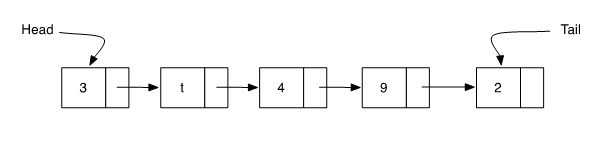
\includegraphics[width=0.5\textwidth]{pictures/linked_list.jpg}
\caption{Single Linked List}
\label{fig:single}
\end{figure}

   

\begin{figure}[H]
\centering
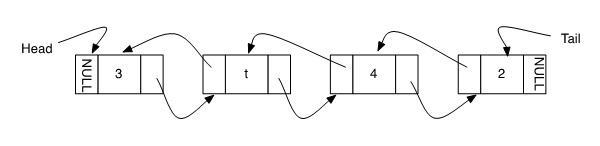
\includegraphics[width=0.5\textwidth]{pictures/double_linked_list.jpg}
\caption{Double Linked List}
\label{fig:double}
\end{figure}


\begin{figure}[H]
\centering
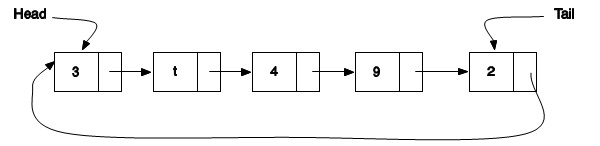
\includegraphics[width=0.5\textwidth]{pictures/circular_linked_list.jpg}
\caption{Circular Linked List}
\label{fig:circular}
\end{figure}

\subsection{Implementation Details}  

When you write the operations for a linked list, the most challenging aspect is to keep track of the pointers that give access to the adjacent nodes in the list.

The pseudocode below illustrates the process for adding an element to the beginning of the list. This pseudocode assumes that currentElement is the beginning of the list and that newElement has already been allocated and is pointing to the list data.  The order of these two lines of code is very important. Can you explain why?     

\begin{lstlisting}
       newElement-$>$next = currentElement-$>$next     
       currentElement-$>$next = newElement
\end{lstlisting}


The following steps are required to add a node to the end of the list:
\begin{enumerate}
\item Initialize a new element with the desired data.  This should be a separate function call.     
\item Walk through until end of list is reached 
\item Set the \textit{next} attribute of the element at the end of the list to the new element.    
\end{enumerate}

The most challenging part of this algorithm is  Step 2, walking through the list.   This is an operation that you will find yourself doing frequently with linked data structures.  The pseudocode for that step is shown below.  Draw a list on some paper and work through the algorithm until you understand how to walk through a list to get to the end of the list.

\begin{lstlisting}
currentElement = firstElementOfList //usually called the head of the list
while(currentElement->next is not NULL)
    currentElement = currentElement->next
lastElement = currentElement
\end{lstlisting}


\subsection{Nodes}
A node, or element,  is the fundamental  structure within a list. Regardless of your choice of implementation for a list, you will need some kind of a node structure to contain the data for the list.

When we take the time to create an ADT, we want it to be truly abstract.  That means that the ADT should not be tied to a particular kind of data, since the operations on a list are identical whether it is storing integers, strings, or structs.   It is a waste of time and testing to create separate ADT libraries for every possible type of data.

Instead we abstract the data by creating a data structure called a \textbf{node}.  As a minimum, the node contains  a pointer that points to the data being stored,  and a pointer to the next node in the list. 

\begin{lstlisting}
typedef struct Node {
    void * data;
    struct Node * next;
}Node;
\end{lstlisting}

The type of the data doesn't matter because it is cast to a void pointer (void *).   The data stored in the list might be a string; it might be an integer; or it might be a complex struct that represents a larger data record about some entity.

A linked list ADT should have a function that creates a new node,  sets the next pointer to NULL, and assigns the data to the data pointer.    Algorithms for working with linked lists assume that the \emph{\textit{next pointer}} for the tail element  is set to NULL so that the end of the list is easily identified.   It is very important to ensure that all new nodes have their next pointer initialized to NULL.

The data stored in a linked list is separate from the node definition.  A node simply points to the data element.  Suppose you were storing addresses in the list. The  data representation would then contain elements for name, phone number, mailing address and possibly email address.   A struct to represent the data might be given as follows.

\begin{lstlisting}
typedef struct Address {
    char * name;
    char * telephone;
    char * mailingAddress;
    char * email;
} Address;
\end{lstlisting}


\subsection{Operations}

A list ADT typically provides functions  that add elements to the list,  remove elements from the list,  report how long the list is,  and possibly sort the list.    It also must provide functions to create and destroy the list.

A minimum set of operations is shown below.  The names of the functions can vary, but an operation with comparable functionality is necessary.    The parameters given in the pseudcode are also a minimum set of parameters.  Implemented functions may need additional parameters. 

\begin{lstlisting}
·create(...): List
·destroy(List)
·insertFront(List,  DataElement):theHead
·getFront(List):DataElement
·deleteFront(List)
\end{lstlisting}


 Once a list is created, it is manipulated  through operations on the ADT functions. These functions and procedures  can do whatever the programmer desires, as long as they are written  carefully to \textbf{encapsulate} the implementation details of the list.   While a list ADT is functional with just the minimum set of functions, usually more functions are provided with an ADT.  Some common additional operations on lists include
 
 \begin{itemize} 
 \item Finding the length of a list
 \begin{itemize}
\item  returns an int and takes the root of the list as a parameter
  \item getLength(List):int
  \end{itemize}
\item Finding an element of a list
 \begin{itemize}
 \item returns a  pointer to the element in the list, without removing the element from the list
\item needs a search criteria and the list as parameters, and returns a pointer to the data element, not the node

\item find(Element, List)
\end{itemize}
\item  Printing a list.
\begin{itemize}
\item might print the entire list to stdout
\item a more elegant version returns a 
             string (or pointer to a string) that represents a nicely formatted 
             printout of the list elements.
\item print(List):char*
\end{itemize}
\item Adding/removing Nodes at the end of the  list

	\item  Adding/removing nodes after or before a 
         specific element
	\item Adding/removing nodes in a specific position in the list
	\item getting the length of the list
	\item {\textbf{Iterator} operations (current, next, previous, head, tail)
	
An iterator is a function that allows the user to step through the elements in a data structure.  Iterators typically “remember” the current position so that the user can move backwards and forwards within the data structure.

}
\end{itemize}

\subsection{Adding Elements}



 Elements can be added into a list at the 
       beginning, in the middle, at some arbitrary location, at the end, etc. 
       Each insert algorithm is slightly different than the others but the 
       basic idea is the same in all cases.


\begin{enumerate}
	\item Construct a new list element
	\item Put the desired data into the new element
	\item Find the location where the element is supposed to be inserted
	\item Adjust the other list elements so that the new one is in the right 
         location and so all existing elements are still part of the list
\end{enumerate}

 Algorithms for inserting an element in  the first position and last position are shown below.  The pseudocode or algorithm for inserting in a specific location is left as an exercise for you to do.


\begin{lstlisting}
insertFirst(List, Element):theHead
Also Known as:addFront, insertFront, addHead, etc
Purpose: To add an element to the list at the front of the list
Preconditions: An initialized list is available.  
PostConditions: The node containing the desired data is added to the front of the list, the length of the list is increased by one, the head of the list is set to point at the newly added element.

insertFirst(List, Element):theHead
     initialize a new node with the desired data
     set the next pointer of the new node to point at the first nod of the list
     set theHead  of the list to point at  the new node
\end{lstlisting}
   
\begin{lstlisting}
insertLast(List, DataElement):void
Also Known as: addBack, insertBack, addTail, etc
Purpose: To add an element to the list at the tail of the list
Preconditions: An initialized list is available.  The new node has the next pointer initialized to NULL
PostConditions: The node containing the desired data is added to the end of the list, the length of the list is increased by one.

insertLast(List, DataElement):void
	initialize a new element with the desired data.  
	walk through until end of list is reached 
	set the next attribute of the element at the end of the list to the new element.    
\end{lstlisting}

\subsection{Deleting Nodes}

Deleting nodes in a list  uses algorithms that are the reverse of adding nodes.  Nodes can be deleted from the front, the back, or any location in the list.   The simplest algorithms delete nodes from the front or the back of the list.  


\begin{lstlisting}
deleteFront(List):Element  //often a delete method returns the value it has deleted
Also Known As: deleteFirst, removeFront, removeFirst
Purpose: To remove the first element from the list and return it to the calling procedure
Preconditions: A non-empty list is available
PostConditions: The first element of the list is removed, the length of the list is decreased by one,  the removed element is returned.

deleteFirst(List):Element
    set a temporary pointer(temp) to point at the first node in the list
   set the head pointer of the list to point at the second node in the list
   set the next pointer of the temporary node (the former first node)  to be NULL
    return(temp->data)
\end{lstlisting}

\begin{lstlisting}
deleteFromBack(List):Element  //often a delete method returns the value it has deleted
Also Known As: deleteLast, removeBack,  etc
Purpose: To remove the last element from the list and return it to the calling procedure
Preconditions: A non-empty list is available
PostConditions: The last element of the list is removed, the length of the list is decreased by one,  the removed element is returned.

deleteLast(List):Element
	walk the list to find the second last element //node->next->next == NULL
    set a temporary pointer(temp) to point at the last node in the list
    set the next pointer of the second last element to NULL
   set the next pointer of the temporary node (the former last node)  to be NULL
    return(temp->data)
\end{lstlisting}


\subsection{Other Core List Operations}

\begin{lstlisting}
isEmpty(List):Boolean
Purpose: To determine if the list has any elements stored in it   
Preconditions: An initialized list is available
PostConditions: None

isEmpty(List):Boolean
    if theHead == NULL and theTail == NULL
    then return (true)
    else return (false)
\end{lstlisting}   


isFull() is a function that is only useful in situations where a list could be 
       full.  This might happen in situations where a specific amount of memory 
       has been allocated to the list.  In that case when the memory is full,  
       a reallocation must be effected before the list size can be increased by 
       adding another element.
\begin{lstlisting}
isFull():Boolean
Purpose:To determine if the list is filled to capacity
Preconditions: An initialized, non-empty list is available
PostConditions: None
   
isFull():Boolean
    if length == maxSize
    then return (true)
    else return (false)
\end{lstlisting}
       

\begin{lstlisting}
create(...): List
Purpose: Create a new List initialized to be empty
Inputs: the function pointers for functions to manage the data stored in the list
Preconditions: None
PostConditions: A new list is created and is empty

create(...):List
    create the struct to hold the list metadata (head, tail, function pointers, etc)
    assign NULL to head (and tail if necessary)
    assign function pointers
    return(List)
\end {lstlisting}


\begin{lstlisting}
destroy(List)
Purpose: To destroy a list, freeing memory if required
Preconditions: A list exists
PostConditions: The list is destroyed

destroy(List)
   for each node in the list
       delete the data in the node using function pointer
       delete the node
   delete the struct holding the list metadata
\end{lstlisting}
   




\section{Array implementation for a list}

The previous sections of this document have focussed on the list composed of linked data structures (the linked list).   A list ADT does not have to be a constructed using linked nodes.   An array can be used to construct a List ADT. At its simplest, the array holds the data in the list and each location in the array is one element of the list. The head of the list is at the first position in the array and the tail of the list is wherever the last element is.  

The array-based list stores void * data in the array in the same way that the linked node stored void * data for the linked data structure.

The choice of implementation does not change the operations required for the list ADT but it does change some of the implementation details.   For example,  if the user wished to insert data into the list maintaining a sorted order, the insert operation would require that room is made for the new element by shifting any subsequent elements one position in the array.   If a data value was to be deleted from the list,  the delete operation must ensure that the space left from the deletion is filled by shifting the tail-end of the array one space towards the head.     

Because arrays must be allocated to be a fixed size in C,  a new longer array must be constructed and the data copied into it if the list grows longer than the size of the array.

Fortunately,  because of information hiding and encapsulation,  the user of the the List ADT should never need to know whether the List is implemented as a linked data structure or an array-based list.


\section{ Array Lists vs Linked Lists}   

\textbf{Linked Lists}
\begin{itemize}
\item Advantages
\begin{itemize}
\item Linked lists can be an arbitrary size because the list grows and  shrinks as elements are added.     
\item Insertion and deletion of data do not require moving  other  data elements, so the operations are more efficient than the comparable operation  on an array structure. 
\end{itemize}
\item Disadvantages
\begin{itemize}
\item Linked lists are less efficient in situations where the program must be able to access any element of the data at any point in the program.  This type of accessibility is called \textbf{random access} and is more efficiently implemented with an array.
\end{itemize}    
\end{itemize}  

\textbf{Array Lists}
\begin{itemize}
\item Advantages
\begin{itemize}
\item Many operations are very fast because the array indices provide direct access
\item functions are simple and easy to debug, making ADT development simpler  
\end{itemize}
\item Disadvantages
\begin{itemize}
\item The resizing operations can be processor intensive if the list is large. There are many different strategies for deciding how much bigger to make the new array when resizing.    
\item To keep an array sorted, you must shuffle the elements each time you add another element.    
\end{itemize}
\end{itemize}

\section{List Iterator}

An iterator is a mechanism that allows navigation of a data structure.   An iterator is usually a different structure (or class in the case of object oriented programs)  that is fairly tightly coupled with the implementation of the data structure being iterated.

When creating an ADT library in C,  iterator functions can be included easily either with, or without the use of additional structures.

List iterator methods permit forwards and backwards navigation of the 
       list. They are extremely useful for accomplishing insertions and 
       deletions because the navigation code is encapsulated within the 
       iterator operation.

Iterator methods for a list might include:
\begin{itemize}
	\item next()
	\item previous()
	\item first()
	\item last()
	\item moveToNth()
	\item getCurrentElement()
	\item setCurrentElement()
\end{itemize}

While some of the iterator methods might seem to be duplicates of the basic list functions,  an iterator has an important role to play in encapsulation.     An iterator can hide the implementation of the list from the user of the library and can provide only the navigational functions to the user.

For example,  an iterator for a list could be set up as follows:

\begin{lstlisting}
typedef struct Iterator
{
    List * theList;
    Node * currentListPos;

}ListIterator;

\end{lstlisting}

Given this structure,  the functions shown above could take a ListIterator as a parameter and provide the user with data that is stored in the list.   Of course, the ListIterator would need to be initialized with enough parameters that it could, in turn, initialize the underlying list.

An algorithm for the \textit{next()} function is shown below.

\begin{lstlisting}
next(ListIterator):DataElement  
Purpose: To move to the next element in a list and return the value of that element
Preconditions: The List member of the ListIterator is non-empty
PostConditions: The currentListPos of the iterator is increased by one and the data stored at that node is returned

next(ListIterator):DataElement  
	if currentListPos is not the end of the list
	   dataToReturn = currentListPos->data
	   currentListPos = currentListPos->next
	return (dataToReturn)
\end{lstlisting}


Some list iterator operations, such as previous() are easier using a double linked list, but all operations are possible regardless of list implementation.   The algorithm for other list iterator operations are left as a practice exercise.

\section{Extending Activities}

\begin{itemize}

\item Write an algorithm for the addToLocation() operation.  This operation should add an element to the list at a specific location in the list (identified by a number). Use the same specification format as has been used to describe operations in this lesson. Include all necessary parameters and return values in the signature of your specification. Be sure to include preconditions and postconditions

\item Write the algorithm to delete a node from the nth position of a linked list.  The operation should return the deleted data and  ensure that the remaining elements of the list are properly connected.

\item Write the algorithm for inserting a node in sorted order given an array implementation of a list.   The algorithm should take the data as a parameter.

\item Write the algorithm for the list iterator operation \textit{previous()}.  It should take a ListIterator as a parameter and return the data associated with the previous node.  It should also adjust the current position pointer.   Write the algorithm for a double linked list and then write it again for a single linked list.

\end{itemize}

%%%%%%%%%%%%%%%%%%%%%%%%
%Stack chapter
%%%%%%%%%%%%%%%%%%%%%%%%

\chapter{Stack ADT}

    A full understanding of the List ADT is needed in order to fully understand stacks.  If you do not understand how lists work and the associated operations of lists, please review that material before attempting to understand the Stack ADT.
    
    
\begin{figure}[H]
\centering
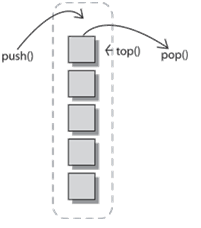
\includegraphics{pictures/stack.png}
\caption{A stack data structure}
\label{fig:stack}
\end{figure}


    A stack is a linear data structure  in which all insertions and
deletions occur at the head, or top of the stack. A stack ADT can only be
interacted with from the front, or top, of the stack. Items can be placed
on the top, and then taken off the top, but never shuffled or sorted
through. A stack of building blocks on a base is a good visual metaphor for
a stack. Imagine that you want to add height to the stack of blocks- you
 add blocks to the top of the stack. To reduce the height of the
stack of blocks, you  remove blocks from the stack.


\begin{figure}[H]
\centering
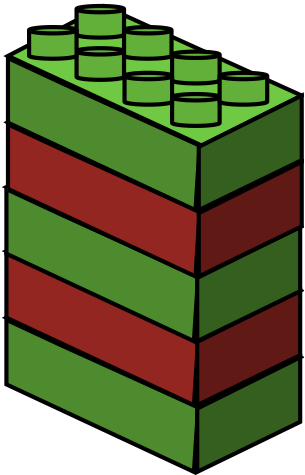
\includegraphics{pictures/stackofbricks.png}
\caption{A stack of bricks}
\label{fig:lego}
\end{figure}



Another good metaphor for a stack is a stack of pennies. If you want a penny of a specific year on top you could remove pennies from the stack until you reach it. If the penny you want is on the bottom of the stack you would need to remove every penny above it in order to get to it. You couldn’t just pull it out from beneath all the other pennies. And no, a stack implementation won’t let you knock over the stack and grab the penny you want.


\begin{figure}[H]
\centering
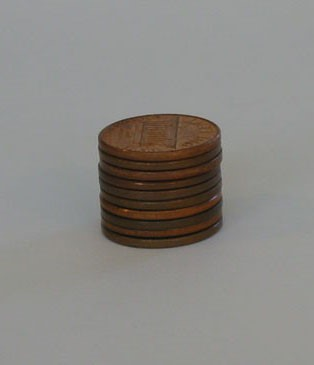
\includegraphics{pictures/pennies.jpg}
\caption{A stack of pennies}
\label{fig:pennies}
\end{figure}

\section{Why use stacks?}

Often programmers feel that if they have one usable data structure  that is enough.  The list ADT is powerful and flexible and many programmers use it for all purposes.  However, there are many times when a special purpose ADT is more appropriate.  Some applications do not require the flexibility of a list, but need to meet speed or data storage requirements.  A specialized ADT can often reduce overhead and speed up operations.  Below are some additional reasons to be familiar with and understand multiple different types of ADTs.

\begin{itemize}
\item A program becomes more readable and errors become easier to find therein if explicit use of specialized data structures is made. 
\item Simpler interfaces (like in the case of the class stack) make specialized implementations possible which are particularly time or space efficient. For example, the Stack ADT could be implemented with the help of a particularly space-efficient list ADT, thus reducing space requirements overall.  
\item The use of a specialized data structure often leads to more insight into the problem definition from which further improvements in the implementation can arise then. 
\item To give an example: That a given stack will store only a certain number of elements known in advance during the overall runtime could be noticed by the programmer only by explicit use of a stack. A b\_stack then would be the structure of choice and its use would imply an improvement of the space efficiency. 
\end{itemize}

\section{Operations on a Stack ADT}
    A Stack is a \textbf{LIFO data structure}. LIFO stands for Last In, First Out. The last element to be placed in the stack will be the first to be removed from it.   
    
    The most modular way to create a Stack ADT is to encapsulate a List ADT. 
To create a stack using an encapsulated list, you simply make use of the operations provided by the LIST ADT. For example, a list ADT might have operations such as addHead, removeHead. Those operations can be used inside the Stack ADT to provide the operations needed by the Stack. 
    Often a Stack ADT is implemented as a \textbf{wrapper}  around a List ADT.   In the same way that the ListIterator used the List ADT and provided  iterator operations to the user while hiding the details of the list from the user,  the Stack ADT uses the List ADT and provides stack operations.

A Stack ADT structure might look as follows:

\begin{lstlisting}
typedef struct Stack
{
    List * theList;
    Node * top;  //top of the stack
    int stackSize;
}Stack;

\end{lstlisting}

The operations provided with any Stack ADT must allow for creation and destruction of the stack as well as insertion and removal of elements as a minimum.   Because the goal is an \textbf{abstract} data type,  the stack must  be initialized with pointers to functions for managing the stored data.   

Since the Stack ADT presented here is a wrapper around a List ADT, most of the stack operations simply call the operations of the underlying list.  The Stack ADT hides the list operations from the user of the stack.

\begin{lstlisting}
create(): Stack
Purpose: To create and initialize a stack
PreConditions: None
PostConditions: A stack is created and initialized to empty

create(): Stack
      create the List sending in the appropriate function pointer parameters
     set the top  pointer to the first position in list
     return (the stack we just created)
\end{lstlisting}


\begin{lstlisting}
destroy(stack)
Purpose: To destroy a stack
PreConditions: An initialized stack exists
PostConditions: The stack is destroyed and all associated memory is freed.

destroy(Stack)
     destroy theList using the list ADT destroy function
     destroy the top pointer
     destroy the stack struct
\end{lstlisting}



The push() function of a stack is equivalent to the addFront() function for  a list.  One of  the  main purposes for creating the specialized ADT is program readability and maintainability so it is important to use function names that are widely associated with the specific ADT.

\begin{lstlisting}
push(Stack, Element)
Also Known As: add, insert
Purpose: Places an element in the stack
PreConditions: The stack is not full
PostConditions: An element is added to the stack, the length is increased by one, the top of the stack points to the newly added element

push(Stack, DataElement)
     insertFront(theList, DataElement)  
     top is set to the position of the data just added
     stackSize is increased by one
\end{lstlisting}


\begin{lstlisting}
pop(Stack): Element
Also Known As: remove, delete
Purpose: Removes the first element in the stack
PreConditions: The stack is not empty
PostConditions: The first (top) element of the stack is removed and returned to the caller. The top of the stack is set to the successor of the removed element, the length of the stack is decremented by one.

pop(Stack):Element
     theRemovedElement  is set to the return value of getFront(theList)
     the first element of the list is removed  by calling removeFront(theList)
     top  is set to  the new first element of theList 
     return(theRemovedElement)
\end{lstlisting}


\begin{lstlisting}
peek(Stack): Element
Also Known As: top
Purpose: To examine the element at the top of the stack without removing it from the stack.
PreConditions: The stack is not empty
PostConditions: Returns the element that is at the top of the stack but does not remove that element from the stack.

peek(Stack):Element
     theValue  is set to point at the data element at position (top) in the list. Sometimes a copy of the data element is made rather than providing a pointer to the actual data element.   Use the list operation getFront(List)
     return (theValue)
\end{lstlisting}




\begin{lstlisting}
isEmpty(Stack): Boolean
Purpose: To determine if the stack is empty
Preconditions: An initialized stack exists
PostConditions: evaluates to true if the stack has no elements, false otherwise

isEmpty(Stack):Boolean
     if(theList is empty)  //use the List isEmpty() function
     then return(true)
     else return(false)
\end{lstlisting}




\begin{lstlisting}
isFull(Stack): Boolean
Purpose: Relevant only in situations where the size of the stack is limited. Is used to determine whether the stack is full.
PreConditions: An initialized stack is available
PostConditions: Evaluates to true if the stack has reached its maximum size, false otherwise.

isFull(Stack):Boolean
     if(theList is full)  or the MAX_SIZE of the stack has been reached
     then return(true)
     else return(false)
\end{lstlisting}


The size of a stack is often an input that is used in algorithms involving a Stack ADT.  As such it is an important piece of data to keep, even if the underlying list implementation does not keep a length.   Stack operations may need to have logic added to update the stackSize struct member.

\begin{lstlisting}
length(Stack): int
Purpose: To obtain a count of the number of elements currently in the stack
PreConditions: An initialized stack is available
PostConditions: returns the count of the number of elements

length (Stack): Int
     return  stackSize  (or theList->length if the list ADT keeps track of length)
\end{lstlisting}



\section{Array Implementation of a Stack}
    Arrays can also be used to create a stack ADT. To use an array as a stack you simply need to ensure that the elements are added to the array sequentially and that your stack ADT keeps track of where the 'top' of the stack is in the array. 
    
 For example, suppose we allocated an array of size 8 to store a stack of
 integers, and a separate variable called top to keep track of the position of the top of the stack. The figure below shows the array after the integer 7 has been pushed onto the stack. The variable top has the value 0 because
    the top of the stack is at position 0 in the array.

\begin{figure}[H]
\centering
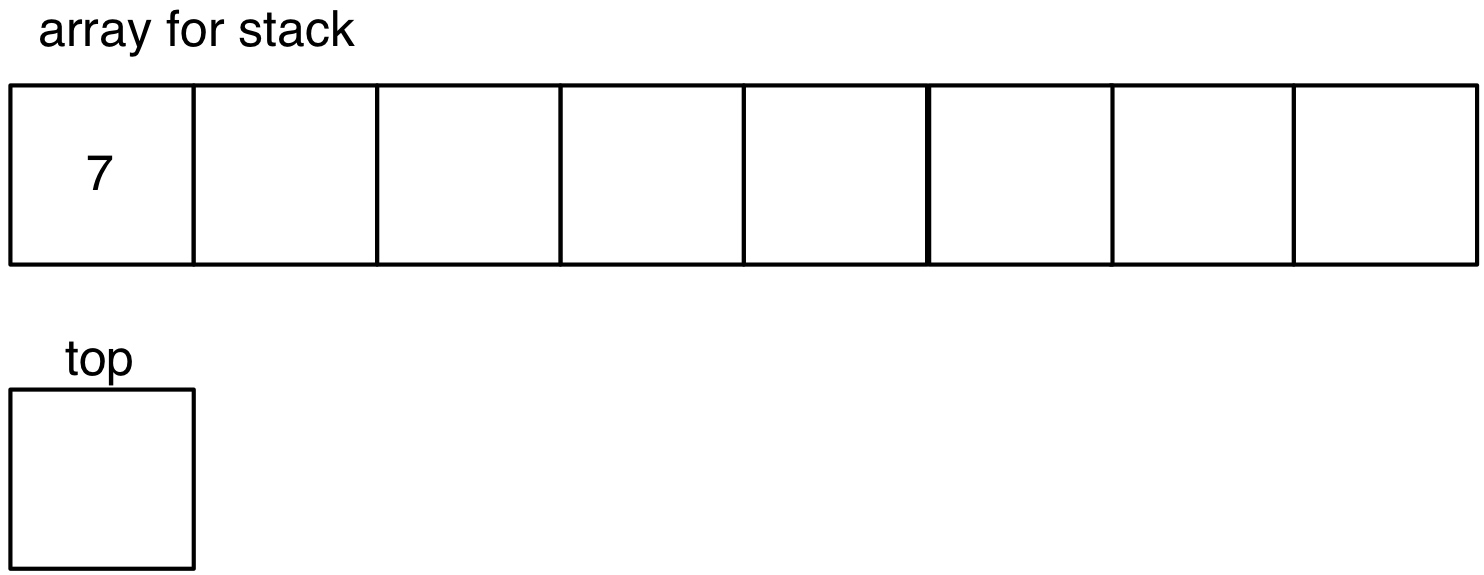
\includegraphics{pictures/arrayStackOne.jpg}
\caption{7 at position 0}
\label{fig:stack1}
\end{figure}
 After three more elements are pushed onto the stack, the array contains four items and the top variable holds the value of 3 because the top of the stack is at position 3 in the array.
\begin{figure}[H]
\centering
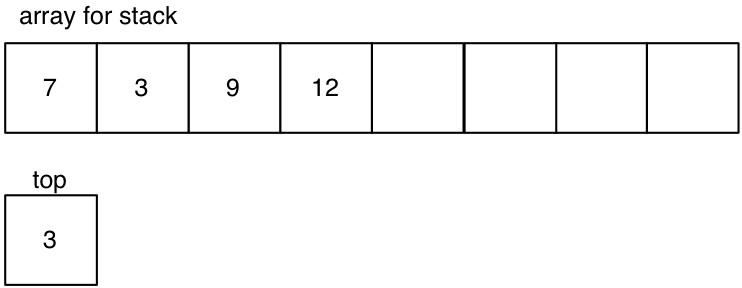
\includegraphics{pictures/arrayStacksTwo.jpg}
\caption{7 at position 3}
\label{fig:stack2}
\end{figure}


If an element is popped off the stack, the array then holds three elements and the top variable would hold the value 2 because the top of the stack moves to position 2 when an element is taken off the stack.

An array implementation of a Stack ADT needs to provide the same set of stack operations as the encapsulated list implementation.   However, the operations will not call list ADT operations, they will directly manipulate the array. Because an array is a fixed size, your ADT will need to provide an isFull operation so that programmers using your ADT can avoid overflowing your stack.

\section{Applications}
    A stack reverses the order of the elements stored. This property makes a
    stack very useful in certain programming applications including memory
    management and many mathematical applications

    It is always a good idea to use the correct data structure for the problem.
    While you could use a list for everything, the use of the more specialized
    data structures makes your code more readable and makes it much easier to
    see errors of logic. A specialized data structure can be created with
    efficiencies designed to make the program faster, or use less memory. Also,
    specialized data structures make it easier for the programmer using the ADT
    to conceptualize the problem. If a programmer is using a stack ADT for a
    program that requires the properties of a stack, then the programmer cannot
    make errors such as taking a data element out of the middle. 



\subsubsection{Reverse Polish Notation (Postfix notation)}
    The most common mathematical notation is \emph{infix} notation. The
    operators appear between the operands for the operation (e.g. 1 + 2, 5 *
    4, a/b). Infix notation is ambiguous by itself and must be annotated with
    parenthesis and a set of rules for the order in which operations are carried
    out.
    
    For example, consider the arithmetic problem 7 * 5 - 4 * 2. The answer
    could be 23 or 61 or ??. The 'right' answer is clear to those who
    understand the order of operations rules.

    A polish logician, Jan Lukasiewicz, developed a notation that does not
    require parenthesis and that embeds the required order of operations in the
    notation. Statements are read from left to right and the previous two
    operands are evaluated when an operator is encountered. The table below
    shows several examples of Infix and the equivalent Postfix notation. \newline

\begin{tabular}{lllll}
\hline
Infix           & Postfix   &  &  &  \\ \hline
a + b           & ab+       &  &  &  \\
(a-b)*c         & ab-c*     &  &  &  \\
(a+b)/(b*a)     & ab+ba*/   &  &  &  \\ \hline
(a*(b+c))/d     & abc+*d/   &  &  &  \\
a*((b-c)/(d+e)) & bc-de+/a* &  &  & 
\end{tabular}
    \newline Consider the second example. Reading left to right, the first two operands are a and b, the next character is a minus sign, so b is subtracted from a giving an answer that is stored as a single operand. The next item read is a c which is an operand. The next item read indicates multiplication so c is multiplied by the next most recent operand, which is the result of subtracting b from a.

    Work through each of the examples in the table so that you are confident in working with postfix notation.

    A stack is the data structure of choice for creating a reverse polish calculator. Each time you read a character from the input stream you push
it onto the stack. When an operation is encountered, you pop two operands
off the stack, perform the operation, and push the result back onto the stack. You then continue reading the input stream.

    Consider, once more, the second example in the table. As the input stream
is read, a is pushed onto the stack, followed by b. The next character is
an operand so two pop operations are executed and a-b is calculated. The
result is pushed onto the stack. At this point the stack contains one
value. The next symbol is read and is pushed onto the stack because it is
not an operand. There are now two elements on the stack. The final symbol
is read, two pop operations are executed and the multiplication operation
is executed.



\section{Resources}
    There are many good resources about stacks on the internet. A few are listed below, but this is only a small sample.   It is worth spending some time to find resources that work well for your personal style of learning.

\begin{itemize}
	\item http://www.cs.bu.edu/teaching/c/stack/array/
	\item http://www.algolist.net/Data\_structures/Stack
\end{itemize}


\section{Extending Activities}

\begin{itemize}
\item Would a double linked list or a single linked list be a better choice for encapsulation in a Stack ADT?  Justify your opinion.

\item Write the algorithms for push() and pop() given an array implementation of a stack.  Show the stack struct definition as  well.

\item Create a design or prototype of a reverse polish calculator program.   You should limit operations to + - * and /.    Use a stack ADT in your design.

\end{itemize}

%%%%%%%%%%%%%%%%%%%%%%%%%%%
%Queues
%%%%%%%%%%%%%%%%%%%%%%%%%%%


\chapter{Queues}
\section{Introduction}

A queue is an example of a \textbf{FIFO data structure}. FIFO stands for First In First Out.   The defining characteristic of a FIFO data structure is that 
the data that has been stored the longest is the next piece of data that will be returned by a 'get data' operation. FIFO data structures do not allow the user to retrieve specific pieces of data.


\begin{figure}[H]
\centering
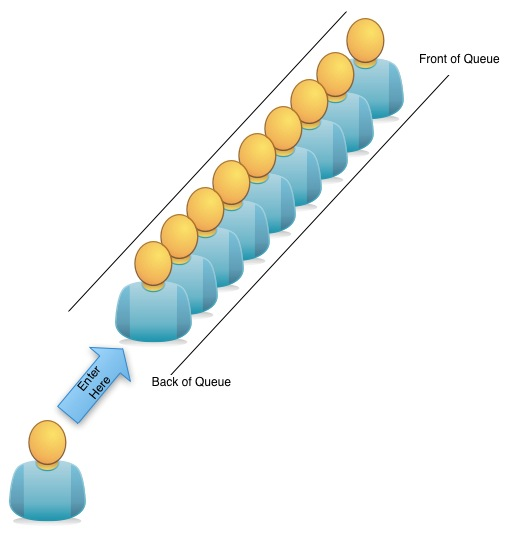
\includegraphics[width=0.5\textwidth]{pictures/queue.jpg}
\caption{Queue}
\label{fig:queue}
\end{figure}

A Queue ADT usually has no size restrictions and can grow or shrink unrestricted. In some applications it is possible to constrain the size of the queue to some predetermined maximum, which allows the software developer to select extremely efficient representations for the queue.

Similar to the Stack ADT, one of the most common implementations for a Queue is the encapsulation of a List ADT.   Because a Queue typically does not have a size, it is most common to use a linked list as the encapsulated ADT but an array implementation of a list could be used where max size is known and the characteristics of arrays give some needed performance advantage.

\section{Implementation: Encapsulate List ADT}

The most modular way to create a Queue ADT is to encapsulate a List ADT. To encapsulate an ADT you write your new ADT using the encapsulated one as a variable or data structure.

The Queue ADT must retrieve data elements from the front of the list (getFront(List)) and add elements at the back of the list (addToBack(List)).    If the chosen List ADT does not provide an addToBack function,  it cannot easily be used as the underlying ADT for a queue. 

 Encapsulation makes it possible to write the Queue ADT operations without worrying about the actual representation or memory management.  By using a good List ADT we ensure that the representation and memory management are handled properly, and we  make use of that to create our Queue.

%\begin{figure}[H]
%\centering
%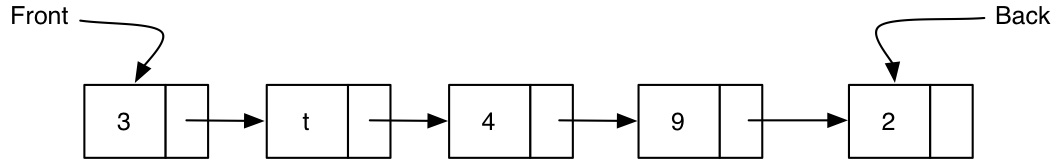
\includegraphics[width=0.5\textwidth]{pictures/linkedlistqueue.jpg}
%\caption{Linked List Queue}
%\label{fig:linkedListQueue}
%\end{figure}


The minimum set of operations on a Queue are:
\begin{itemize}
\item create()
\item enqueue()  //AKA add()
\item dequeue() //AKA remove()
\item destroy()
\end{itemize}


Other optional but useful operations allow the programmer to examine the front of the queue, determine the length of the queue, discover whether the queue is full or empty, etc.

The encapsulated Queue ADT is usually represented by a struct that is accompanied by several functions.  One possible representation of the struct is shown below.

\begin{lstlisting}
typedef struct Queue{
    List * theList;
    Node * front;
    Node * back;  //back is optional
    int * length;
}Queue;
\end{lstlisting}




\begin{lstlisting}
create(): Queue
Purpose: To create and initialize a queue
PreConditions: MAX\_LEN has been defined previously (it could be passed in as a parameter if desired)
PostConditions: A queue is created and initialized to empty


create(): Queue
     theList  is set to point at the return value from create a list- sending in the appropriate function pointers
     front  is set to point at the first position in list
     back  is set to point at the last position in list  //back is an optional pointer
     return (the queue  just created)
\end{lstlisting}




\begin{lstlisting}
destroy(Queue)
Purpose: To destroy a queue
PreConditions: An initialized queue exists
PostConditions: The queue is destroyed and all associated memory is 
       freed.

destroy(Queue)
     destroy theList using the list ADT destroy procedure
     destroy the front and back pointers
     destroy the Queue struct
\end{lstlisting}

   

\begin{lstlisting}
add(Queue, DataElement)
Also Known As: insert(), enqueue()
Purpose: adds an element to the end of the queue
PreConditions: The queue is not full
PostConditions: The new element is added as the last element in queue

add(Queue, Element)
      insertBack(theList, DataElement)
      back pointer is set last position of theList
      length of queue is updated
\end{lstlisting}


\begin{lstlisting}
remove(Queue):DataElement
Also Known As: delete(),  dequeue()
Purpose: removes the first element in the queue
PreConditions: The queue is not empty
PostConditions: The first (front) element of the queue is removed and 
       returned to the caller. The front of the queue is set to the successor 
       of the removed element.


remove (Queue): Element
     theRemovedElement <- getFront(theList)
     remove the first element from the list
     front is set to point at the new first element of theList
     length of the queue is updated
     return(theRemovedElement)
\end{lstlisting}





\begin{lstlisting}
peek(Queue):Element
Also Known As: front()
Purpose: To examine the element at the front of the queue without 
       removing it from the queue.
PreConditions: The queue is not empty
PostConditions: Returns the element that is at the front of the queue 
       but does not remove that element from the queue.

peek(Queue):Element
     return(getFront(theList)
\end{lstlisting}




\begin{lstlisting}
isFull(Queue):Boolean
Purpose: Relevant only in situations where the size of the queue is 
       limited. Is used to determine whether the queue is full.
PreConditions: An initialized queue is available
PostConditions: evaluates to true if the queue has reached its maximum 
       size, false otherwise.
       
isFull():Boolean
     if(theList is full)  OR MAX_SIZE has been reached
     then return(true)
     else return(false)
\end{lstlisting}

  


\begin{lstlisting}
isFull(Queue):Boolean
Purpose: To obtain a count of the number of elements currently in the 
       queue
PreConditions: An initialized queue is available
PostConditions: returns the count of the number of elements

isEmpty():Boolean
     if(theList is empty)
     then return(true)
     else return(false)
\end{lstlisting}




\begin{lstlisting}
length(Queue):int
Purpose: To obtain a count of the number of elements currently in the 
       queue
PreConditions: An initialized queue is available
PostConditions: returns the count of the number of elements

length(Queue):int
     return length OR length(List) if the list ADT provides a length function
\end{lstlisting}

\section{Array Implementation of a Queue}
Queues can be implemented using an array in much the same way as a Stack ADT can be implemented with arrays.

\begin{figure}[H]
\centering
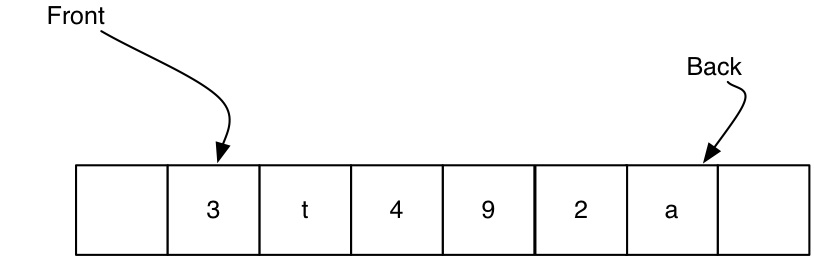
\includegraphics[width=0.5\textwidth]{pictures/arrayBasedQueue.jpg}
\caption{Array Queue}
\label{fig:arrayQueue}
\end{figure}

The programmer must keep track of the front and the back positions of the queue and, if a linear array is used, items must be shuffled up periodically in order to avoid using up all the memory in the computer.

In the example above, the array allocated to the queue has two empty spaces, one at the front and one at the back. One more element can be added to the back of the queue, and then all of the elements will need to be shuffled forwards in the queue in order to add a second additional element.

Removing the element 3 from this queue will free up one more space, but the entire set of elements will have to be shuffled forwards in order to use that space.


\begin{figure}[H]
\centering
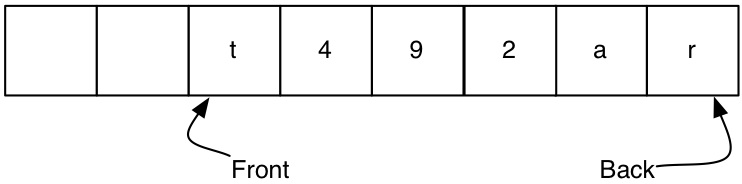
\includegraphics[width=0.5\textwidth]{pictures/arrayQueue2.jpg}
\caption{Array Queue Before Shuffling}
\label{fig:arrayQueue2}
\end{figure}

Shuffling the elements forward is a simple algorithm, but requires that every element is moved, which can take some time if the queue is several thousand elements long. The diagram below shows that there are two spaces at the end of the queue after elements are shuffled forwards.


\begin{figure}[H]
\centering
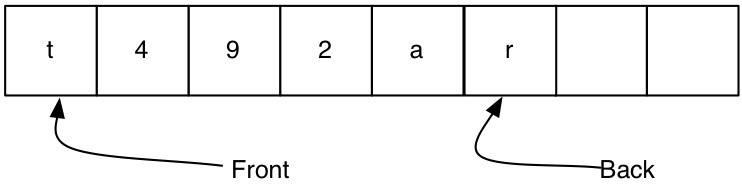
\includegraphics[width=0.5\textwidth]{pictures/arrayQueue3.jpg}
\caption{Array Queue After Shuffling}
\label{fig:arrayQueue3}
\end{figure}



While the array implementation is conceptually simple to describe to collaborators, it comes with several complications as well.  The array implementation can use extra memory if many items are added to the queue and then many are removed.  The queue must either be firmly limited in size or memory must be reallocated as the queue grows and memory reallocation affects the running time of the algorithm.

A common model for an array implementation of a queue is to use a circular buffer as the representation for the queue.

A circular buffer is really just an array, but the method of dealing  with the start and endpoints of the queue is slightly different. Imagine an array, but one that is arranged in a circle. Consider the picture below. The queue contains eight elements, beginning with an 'a'. After removing one element, and adding two more elements the queue will look like the second picture and has two spaces available for additional elements.

\begin{figure}[H]
\centering
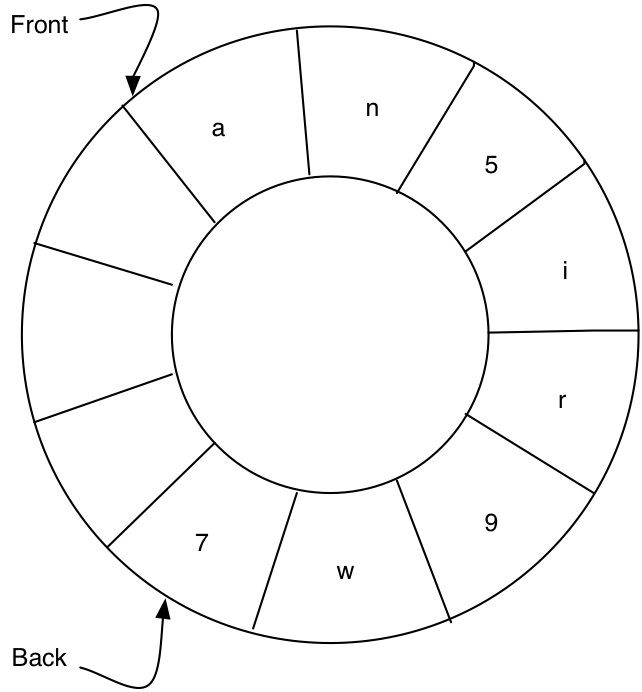
\includegraphics[width=0.3\textwidth]{pictures/circularbufferone.jpg}
\caption{Circular Buffer Queue Before}
\label{fig:circleQueue1}
\end{figure}

\begin{figure}[H]
\centering
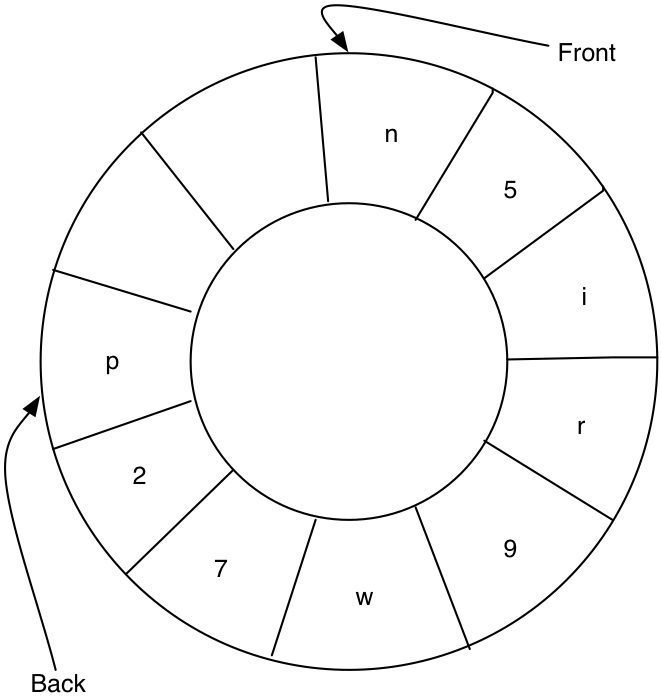
\includegraphics[width=0.3\textwidth]{pictures/circularbuffertwo.jpg}
\caption{Circular Buffer Queue After}
\label{fig:circleQueue2}
\end{figure}



One of the advantages of a circular buffer is that there is no need to shuffle elements around as there is with an array. One of the disadvantages is that the queue must be a fixed length, else the circular buffer suffers from the same memory reallocation requirements as a linear array implementation.

Of course, computer memory isn't circular, so a 'circular' buffer is really implemented using a linear array.


\section{Additional Resources}

\section{Extending Activities}

\begin{itemize}
\item Read the first few sections of the Computational Complexity chapter of this work.  Be sure you understand how to represent the complexity of an algorithm using \textbf{Big O} notation.     What is the complexity of the enqueue() and dequeue() operations?

\item What additional information must be kept track of in order to use a 
       conventional array as a circular buffer?  Give the Queue struct that you would use if you were writing a circular buffer queue implementation.

\item Write the algorithm for dequeuing an item from a circular buffer queue.

\item Which of the following statements about queues is untrue?

\begin{itemize}
\item a) Queues can have elements inserted at any position in the data 
       structure.

\item b) The first element inserted into a queue will be the first element 
       taken out of the queue.

\item c) Queues can be found in the real world.

\item d) The size of a queue data structure is bounded only by the size of the 
       computer memory.

\item e)A queue is somewhat similar to a stack.

\end{itemize}

\item Which List operation would be most likely to be the one encapsulated if you were writing a remove operation for a queue?
\begin{itemize}
\item a) addHead(elementToBeAdded)

\item b)length()

\item c)removeBack()

\item d)removeHead()

\item e)insert(position, elementToBeAdded)
\end{itemize}





\item Given the following queue:  A B b E r S T,  where A is the front of the 
       queue,  what will the queue content be after two remove operations?
\begin{itemize}
\item a)  A B b E r S T

\item b) b E r S T

\item c) A B b E r S

\item d)  T A B b E r S

\item e) The queue will be empty

\end{itemize}




Given the following queue: t y 5 8 i 2 d t e,  what should a call to 
       length() return?
\begin{itemize}
\item a)9

\item b) 8

\item c) 10

\item d) it will generate an error because of the mixed data types

\item e) 3
\end{itemize}

\end{itemize}

\chapter{Associative Arrays} \label{associative}
\section{Introduction}

An associative array is a data structure that lets you manage pairs of data.   Each data pair consists of a key and a value,  where the key is a unique identifier and the value might repeat.  An associative array does not permit the collection of data to have duplicate key values.   For example, if we were storing a collection of data that consisted of student numbers and student names an associative array might be suitable.   Student id numbers are unique within the university so we could guarantee that there would not be any duplicate numbers.  The student number would be the key in this example and the student name would be the value.  It is perfectly permissible for values to repeat.  For example, it is very likely that there would be many students with names like Erin or Lynne.


Student records are a good example of data that is easily stored in an associative array. The student ID (your student number) is the key, and the other data about you (your name, your program, your GPA, etc) forms the value. It is common to have a complex data type (a struct in C) as the value in an associative array.

\section{Implementation}
Associative Arrays can be implemented using a simple array, lists, hash tables and a variety of trees. In this section we look briefly at the array and list implementations. 


\subsection{Array Implementation}

An array implementation of an associative array is useful when the keys for the key/value pairs can be restricted to a finite size and the key of the data pair is  an integer because the keys are used as the indices into the array.         

The picture below shows an array based associative array. The left hand column is just to illustrate the position of the data and would not be stored separately. The 'key' would simply be the index into the array.



\begin{figure}[H]
\centering
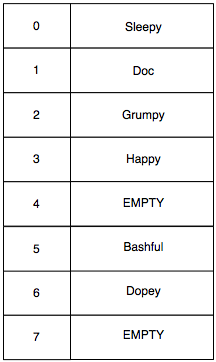
\includegraphics[width=0.3\textwidth]{pictures/image004.png}
\caption{Array Implemented Associative Array}
\label{fig:aa2}
\end{figure}

A sentinel value is used when there is no value for the key (The sentinel values is EMPTY in the example picture).      

\begin{itemize}
\item Advantages:
\begin{itemize}
	\item An array based implementation gives very fast operations because most require only a simple index into the array (O(1)).         
	\item The array based implementation is also simple and easy to understand.
\end{itemize}

\item Disadvantages:
\begin{itemize}
	\item The entire storage space must be created and initialized to EMPTY, meaning that the storage requirements are quite large compared to other implementations, especially if the set of possible keys is large.
\end{itemize}
\end{itemize}

\subsection{Linked List Implementation}


A linked list implementation of an associative array can use  a specialized list node that contains  the key value as an integer as well as pointers to the one to the next item in the list and  the associated value.

Note that there is no \textbf{requirement} to keep a linked list table sorted in any particular order (in the picture below the list is not sorted by the key) but it often improves performance if the list is kept sorted.

\begin{figure}[H]
\centering
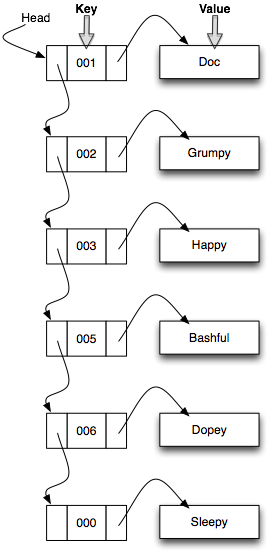
\includegraphics[width=0.3\textwidth]{pictures/image006.png}
\caption{Linked List Implemented Associative Array}
\label{fig:aa3}
\end{figure}

The picture shows a associative array that is a single linked list where the key is stored in the list node along with a pointer to the value. What would be the challenge if you tried to simply use the position of the node in the list as the key? \newline
The struct for a linked version of an associative array might look like this:

\begin{lstlisting}
struct aarray{
    int * key;
    node * next
    void * data
    };
\end{lstlisting}

The reason for adding the key explicitly into the struct rather than leaving it as part of the void*data is that the operations on the array need to compare the key value and would not be able to do that if the key was hidden in the abstracted data.

\begin{itemize}
\item Advantages:
\begin{itemize}
	\item The size of the associative array can grow arbitrarily
	\item The keys do not need to be restricted to a simple integer- for example the key could be a unique alphanumeric
\end{itemize}

\item Disadvantages:
\begin{itemize}
	\item The cost of each operation is dependent on the size of the associative array
\end{itemize}
\end{itemize}

\section{Operations on Associative Arrays}
Operations List (Minimum Set):
\begin{itemize}
	\item create(): AArray
	\item destroy(AArray)
	\item insert (AArray, key, value) 
	\item remove(AArray, key)
	\item lookup(AArray, key):value
	\item update(AArray, key, newValue)
\end{itemize}

\begin{lstlisting}
create():AArray
Purpose: to create an empty, initialized associative array
Preconditions: none
Postconditions: an empty, initialized associative array is created

create():AArray
      1. create the storage ADT
      2. create the key ADT
      3. return(the AArray we just created)
\end{lstlisting}


\begin{lstlisting}
destroy(AArray)
Purpose: to destroy an associative array and free the  memory if required
Preconditions: an initialized associative array
Postconditions: the array  is destroyed along with all references to data. (Important note: the data itself may not be destroyed by this operation and should be removed prior to destroying the AArray).

destroy(AArray)
      1. the appropriate destroy procedure
      2. release any other pointers
\end{lstlisting}

\begin{lstlisting}
insert(AArray, key, value)
Purpose: To add a key/value pair to the associative array
Preconditions: no value exists for the key being added
Postconditions: the size of the AArray has increased by one, the key and value are stored with a reference leading from key to value.

insert(AArray,key,value)
      1. key into key ADT 
      2. connect key and value with reference (pointer)
      3. increase length counter of AArray by one
\end{lstlisting}


\begin{lstlisting}
remove (AArray,key): value
Purpose: to remove a key/value pair from the associative array
Preconditions: the  key/value pair is stored in the AArray
Postconditions: the key/value pair is no longer in the AArray. The length of the AArray has decreased by one.

remove (AArray,key): value
      1. look up key in key ADT
      2. follow reference to value in value ADT
      3. store value in temporary variable
      4. remove value from value ADT
      5. remove key from key ADT
      6. return(temporary variable)
\end{lstlisting}


\begin{lstlisting}
lookup (AArray, key): value
Purpose: to retrieve the value stored for a particular key
Preconditions: the key/value pair is in the AArray
Postconditions: the value is returned. The AArray is unchanged.

lookup (AArray,key): value
      1. look up key in key ADT
      2. follow reference to value in value ADT
      3. store value in temporary variable
      4. return(temporary variable)
\end{lstlisting}


\begin{lstlisting}
update (AArray, key, newValue)
Purpose: the change the value associated with a key that already exists in the associative array
Preconditions: a key/value pair exists for the given key
Postconditions: the new value is associated with the given key


update (AArray, key, newValue)
      1. look up key in key ADT
      2. follow reference to value in value ADT
      3. set value to newValue
\end{lstlisting}


\begin{lstlisting}
exists(key):Boolean
Purpose: to determine if a key is represented in the associative array
Preconditions: an initialized AArray is available
Postconditions: n/a

exists(key):Boolean
      1. look up key in key ADT
      2. if key is found return(true)
      3. else return(false)
\end{lstlisting}


\begin{lstlisting}
isEmpty():Boolean
Purpose: to determine if any key/value pairs are represented in the associative array
Preconditions: an initialized AArray is available
Postconditions: n/a

isEmpty():Boolean
      1. if the key ADT is empty; return(true)
      2. else return (false)
\end{lstlisting}


\begin{lstlisting}
isFull():Boolean
Purpose: to determine if the AArray is full
Preconditions: an initialized AArray is available
Postconditions: n/a

isFull():Boolean
      1. if the key ADT is empty; return(false)
      2. else return (true)
\end{lstlisting}


\section{Applications}
Associative arrays are useful in any situation where you need to maintain a connection between two pieces of data, but where the data might be changed frequently during the running of the program. As an abstract example, AArays are less appropriate for connections between a person and their phone number- which typically stays the same, and more appropriate for representing the connections between a parking lot ticket number on a vehicle and a parking spot.    

Associative arrays are really only useful if the  key portion of the key-data pair maps nicely to the positions in an array.   This is most likely to occur in situations where data is generated sequentially,  such as ticket numbers for a coat check,  or order numbers for an online store.

\subsection{Lending Library}

Scenario: Suppose you wanted to implement a lending library for your collection of computer games so that each game could only be lent out to one person at a time (no copies allowed). The core data structure used by this application could be an associative array.


Requirements: 
\begin{itemize}
	\item Each computer game is assigned a unique ID number (0-N)
	\item Borrowers can have more than one game checked out at a time
	\item A game can only be checked out by a single borrower at any one time
\end{itemize}

\subsubsection{Context}

The application would obviously need some user interface constructs to enable data entry and some file storage utilities to permit persistent storage. For the purposes of this example, we will assume those details have been worked out already.


Programming Constructs we would need to write this program
\begin{itemize}
	\item A way of creating borrowers
	\item A way of identifying borrowers 
\begin{itemize}
	\item The set of borrowers will also need to be in an ADT. If you give each borrower an ID, then an AArray might be a good choice for this as well.
\end{itemize}
	\item A way of creating and populating the list of games that can be borrowed
	\item The AArray representation for the set of borrowed games
\end{itemize}


\subsubsection{Worked example}

Lending Library pseudocode
\begin{itemize}
	\item Create and populate borrowers data structure
	\item Create and populate the games data structure
	\item Initialize the AArray  of borrowed games to empty
	\item If a game is borrowed add the game/borrower pair to the AArray representing the borrowed games
	\item if a game is returned remove the game/borrower pair from the AArray representing the borrowed games
\end{itemize}


\section{Extending Activities}
\begin{itemize}

\item {
If you were implementing a student record system for a small music  school with fewer than 200 students, and were using associative arrays as the data structure, how would you implement your associative array? Would you make a different choice if your student record system was for a university?

}

\item {
Write a 'todo list' of the things you would need to do (including research and learning) in order to implement the borrowers library example.Try to make the list very specific. Use the todo list to estimate the amount of time it would take you to implement and test the application (round up to the nearest hour).
subsubsection

}

\end{itemize}
\chapter{Hash Tables} \label{hash}
\section{Introduction}
 
A Hash Table is an array (aka Table) that uses a hash function to map keys to a specific location in the array.   The position of the entry in the table is determined by the value of the key.  
 
 A hash table (also knowns as a Hash Map)  is a more flexible version of an associative array that does not require that the key of the the key-data pair be something that easily maps to a position in a table.   Instead, the hash table calculates the table position by algorithmically manipulating (hashing) the key to determine the correct position in the table.   A hash table is useful in situations where the data key-value pairs might not have key values that are nicely distributed to allow them to be mapped to table positions between 0 and the end of the table.
 
 
The \textbf{Hash Function} a function that, when given a key as a parameter returns  an integer within a  fixed range.   The hash function ALWAYS returns the same value for a given input, but may return the same value for more than one input.   For example,  a hash function could take in the province and plate number from a car licence plate (something like ONBWCC123) and manipulate the digits and letters to produce an integer that maps to a position on the table.  If the hash table were of size 357, the integer would be between 0 and 356.  

\begin{figure}[H]
\centering
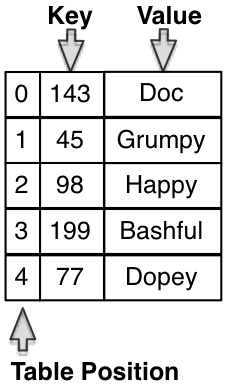
\includegraphics[width=0.3\textwidth]{pictures/Hash_Tables_0.png}
\caption{Hash Table}
\label{fig:hashTable}
\end{figure}

Image \ref{fig:hashTable} shows a 3x5 table.  The first column is labeled as Table Position, the second shows the key, the third shows the value.  There are five sets of data in the table.  

The hash table shown is a simplified table that has the data stored directly in the table.  A finished implementation of a hash table ADT would store void * data in the same way that a linked list does.   A hash table is nearly always implemented using an array, since the primary purpose of using a hash table to facilitate speedy lookups for data.

\paragraph{Real World Example:}
 
Spelling checkers are an application that can employ a hash table.   Because the dictionary of properly spelled words can be quite large,   a search through that dictionary for each word in the document being checked is the most time consuming part of the operation.   The dictionary can be read once into a hash table, where each word in the dictionary is put through a hash function and stored in the table at the appropriate position.  In this example the word is both the key AND the data.
After the table is loaded each word of the document to be spell checked is hashed

\section{Hash Table Operations}
The minimum set of operations for a hash table are exactly the same as the operations for an associative array.
     
The only change is the process for inserting and finding data because the hash table must use the hash function to determine where the new data goes and where the data can be found.
   
The implementation of the operations changes depending on the collision resolution strategy chosen.

Operations List (Minimum Set):  
This is exactly the same operations list is for an associative array.   The algorithms for the operations are also the same and are not repeated here.
\begin{itemize}
\item create(): HTable
\item destroy(HTable)
\item insert (HTable, key, value)
\item remove(HTable, key)
\item lookup(HTable, key):value
\item update(HTable, key, newValue)
\end{itemize}


\section{Hash Table Characteristics}

Hash tables are relatively simple to implement and provide operations that are ideal for tasks that involve frequent look ups of the elements.  Hash tables have several characteristics that  distinguish them from other data structures.


\begin{itemize}
\item Hash tables can provide an improvement over the search time for binary trees ( binary tree search time is O(log 2 n).     The cost of search in a hash table is the time to execute the hash function + any time to resolve collisions which is usually O(1).
\item Hash tables are efficient for large sets of data, but sometimes the hash function is computationally expensive which makes other data structures more effective for small sets of data.
\item The most often used operations on a hash table are the operations for finding and inserting.   These operations are dependent on the hash function.   The selection of hash function is key to the efficient operation of the hash table.
\item The set of keys for the data is called the key space.   The key space is often larger than the size of the table in memory (the address space), which means that often two elements must hash to the same location.  When this happens the collision resolution strategy is used to ensure that both elements are stored and can be retrieved.

\item The hash function maps the key space into the address space.   More specifically the hash function takes a key and uses it to produce an address that is in the defined address space of the allocated table.   The same address must be produced every time given the same key.
\item Because the key space is typically larger than the address space, more than one key will be mapped to the same address.   This is called a collision and must be handled through collision resolution. The selection of collision resolution method is an important part of hash table design.
\end{itemize}


\section{Hash Functions}

The hash function must map the keys in the data to a position in the table.   A hash function needs to know the size of the table (usually sent in as a parameter) in order to determine the appropriate position.
     
The characteristics of a good hash function are:
\begin{itemize}
\item speed: the function cannot be slow to run
\item space: the hash function should not take a lot of storage space
\item generation of positions: the function should spread the keys out evenly across the whole hash table (no clustering in one part of the table)
\end{itemize}

All hash functions take in a key of a particular type as a parameter and return a value between 0 and the size of the table.   Some hash functions are written with a hard coded table size,  some take the table size as a parameter.  Some hash functions work on numeric keys,  some work on alphanumerics.   There are many different possible hash functions.  The subsections below detail some possible approaches to writing hash functions.

\subsection{Before Hashing: Preconditioning}

     Keys in the key space frequently contain alphanumeric characters, but hash functions are often more effective on keys that can be manipulated numerically. One common approach to hashing is to convert alphanumeric keys to a numeric value through a process called preconditioning. Preconditioning can be as simple as replacing each letter with the ascii code for the  letter, or it can do more complex manipulations such as normalizing the length of the keys in addition to converting them. 
   
\subsection{ Hashing by Truncation}

    The \textbf{truncation} method of hashing simply uses a portion of the key as the 
       address space and ignores the rest of the key.  This method is also known as \textbf{Digit Analysis}
       

     The truncation method only works for keys that have consistent characteristics.  For example, suppose you had a set of 8 digit keys such as 46 234 789 and your hash table size was 1000 (hash values between 0 and 999).
     
     One approach to truncation for hashing this number could be to simply select the 1 $^st$ , 3 $^rd$ and 5 $^th$ digits of the key (424 in this case). Another approach to truncation for hashing this type of key could be to select the first, third and last digits and then reverse the order (924 in this case).
     
The approach to truncation must be consistently applied to every key and must always give the same results, but otherwise any sort of digit manipulation that results in a suitably sized address space can be considered as an approach to truncation.

The truncation method has the advantage that it is very fast, but it often results in many collisions because the hashed values often don’t distribute well within the entire table.

\subsection{Hashing by Folding}

The \textbf{folding method} of hashing involves separating the key into parts that are the same length as the address space and performing some kind of math on those parts.  Often one part is composed of the ‘leftovers’ and is a different length.  A common method of folding is to add the parts together once the parts are identified, ignoring the final carry.   The result is used as the table address for the original key.


For example, suppose that the key value of 456 987 321 must be hashed into a table of size 1000 (hash values between 0 and 999). The original key is partitioned into three segments, each three digits long and those segments are added together. 456 + 987 + 321 = 1764. The 1 thousand is ignored and the hash key becomes 764.

The folding method is a fast hashing algorithm and results in more evenly distributed addresses than truncation.  Even though it is better than truncation, it can still result in poorly distributed addresses.

\subsection{Hashing by Division}

Integer division can be used to consistently reduce a large integer to a small one.  Recall the modulo operator, which is used to find the remainder value after integer division.   15 modulo 4 (15\%4) yields the value 3.    The only possible values from an expression that is modulo 4 is 0, 1, 2 or 3.    If we use larger numbers,  say 10000 modulo 999,  the remainder value will have to be  a number between 0 and 998.  We can use this characteristic of  modulo to calculate a hash value of a large number.

The division method hash function calculates the hash value of a key, H(k) by finding the remainder that results from dividing k by some positive integer (modulo). More formally \textbf{H(k) = ABS(k)\%m} where m is a large positive integer, \% is the modulo operator and ABS is the absolute value.

 The division method of hashing will return addresses that are between zero and one less than the divisor (m), so it is important that m is also the size of the table, otherwise this method will result in invalid addresses.


 This method will map keys that are close in value to different addresses, but will map keys that are multiples of each other to the same address, so its effectiveness depends on the characteristics of the original key space. Consider the hash values calculated below, for an m value of 11.
   


\begin{tabular}{lllll}
\hline
Key & Hash  \\ \hline
12  & 1     \\
13  & 2     \\
14  & 3     \\ \hline
56  & 1     \\
57  & 2     \\
58  & 3     \\
239 & 8    
\end{tabular}

The division method can result in very good distribution of address locations depending on the value chosen for m.  The table size (m) should not be set to an even number, or a power of 2 or 10.   Prime numbers, and odd numbers  whose factors are all over 20 are good choices for the table size (m).
   

\section{Collision Resolution for Hashing}

When two keys hash to the same table position we say that a \textbf{collision} has occurred.  Even if the keys for the data are unique, it is likely that sometimes the hash function will calculate the same table position for two keys.   When  this happens, the hash table must find a different location to store the second set of data, since two pieces of data cannot be stored in the same memory location.   The process of locating the alternate storage location is called \textbf{collision resolution}.
   
Two common approaches to collision resolution are \textbf{open addressing} and \textbf{separate chaining}.  Open addressing solutions use an algorithm to search in a repeatable fashion for an alternate location.   Separate chaining solutions create additional table space by using a linked data structure.

\subsection{Open Addressing}

     When a collision occurs in an open addressing hashing system, the collision is resolved by trying alternative cells until an empty cell in the hash table is found. In effect some number is added to the calculated cell position to arrive at a new cell to try, and the formula is set to wrap-around to the beginning of the table when the end is reached.
   
     The number of filled cells in the hash table is used to calculate the \textit{load factor} of the table (number filled/size of table). Open addressing is a collision resolution technique that works best with a table that has a load factor of .5 or less.
   
     The offset is calculated by a collision resolution algorithm. A collision resolution algorithm must ensure that it always finds an empty cell if one is available. We will examine three open-addressing collision resolution algorithms that are used : linear probing, random probing, and double hashing.   There are many more possible approaches and several variations on the three we will examine, but these three serve to illustrate the concepts behind open addressing to resolve collisions.
   
Suppose that the items in the table are names.
\begin{itemize}
\item Sleepy is hashed to position 0
\item Doc and Grumpy are hashed to position 3
\item Sneezy is hashed to position 4
\item Happy is hashed to position 5
\item Bashful and Dopey are hashed to position 7
\end{itemize}



The table state, after each addition is shown in the diagram below.


\begin{figure}[H]
\centering
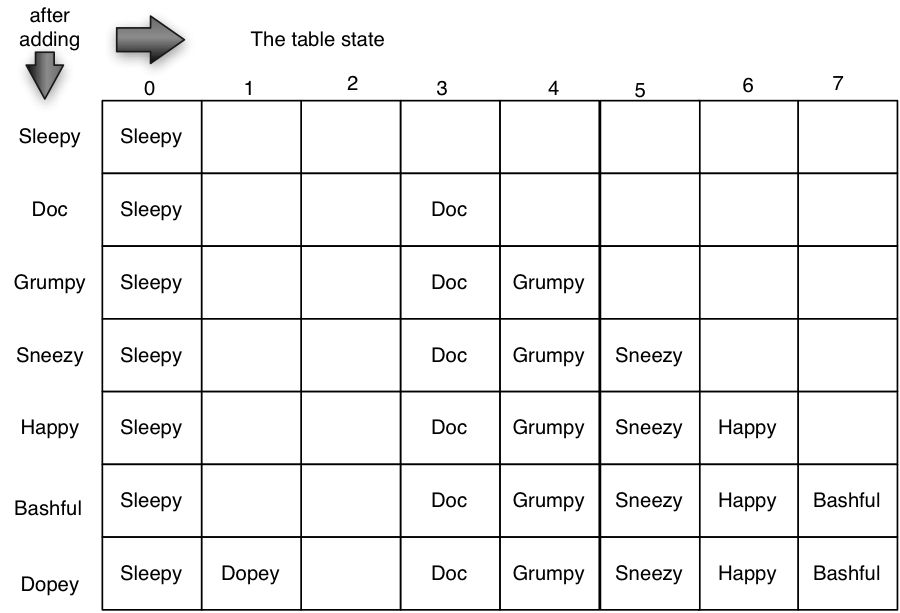
\includegraphics[width=0.5\textwidth]{pictures/Linear_Probing_0.png}
\caption{Linear Probing}
\label{fig:linearProb}
\end{figure}


 While linear probing always finds a cell if one is available, it tends to cluster the data (as you can see in the diagram). This type of clustering is called \textbf{primary clustering}. Also,  as the table gets full, the number of probes required increases which slows down insertions and searching.
   
\subsubsection{Random Probing}


 One way to avoid primary clustering is to change the probing mechanism so that it does not return consecutive positions. The probing strategy cannot truly be random because must still generate every position in the table exactly once for any given collision, and it  must generate exactly the same sequence again given the same collision.  However, it does not  need to generate new table positions  in the order that they appear in the table.
   
One example of such a strategy adds some positive number  to the  location of the collision, and then finds the modulo value with respect to the table size.

\begin{lstlisting}
{ newLocation = (mostRecentLocation + constant) mod tableSize}
\end{lstlisting}


This strategy works well when the constant and the tableSize share no common divisor other than 1. Random probing suffers from \textbf{secondary clustering}.   Secondary clustering occurs when the same exact sequence of  positions is generated   when two keys are mapped to the same position more than once during a search for position. 
   


\subsubsection{Double Hashing or Rehashing}

Double hashing is an effective collision resolution strategy that avoids clustering. When there is a collision of hashed values for keys, the colliding key is hashed again using a different hash function.   The result of the second hash function is not used as a position, but is used as  the constant value in the equation for random probing.
   
\begin{lstlisting}
newLocation = (mostRecentLocation + valueFromSecondHashFunction) mod tableSize
\end{lstlisting}



\subsubsection{Linear Probing}

     Linear probing is a strategy that  places the collided data in the next available cell.  When the end of the table is reached, the search wraps around to the beginning of the table.
     




Double hashing usually eliminates clustering in the hash table because the sequence of values generate for any two colliding keys will not be the same.





\subsection{Separate Chaining}


 Separate chaining is another approach for handling hashing collisions. Rather than try to find an alternate table position, the separate chaining approach stores  the colliding records for a single table  position in a linked list.  Instead of storing data directly in the hash table, the linked list is stored in the hash table at the hashed position.   The separate chaining method requires memory storage space for the hash table as well as for the linked lists, so it is more memory intensive than an open addressing approach to collision resolution.  
   


\begin{figure}[H]
\centering
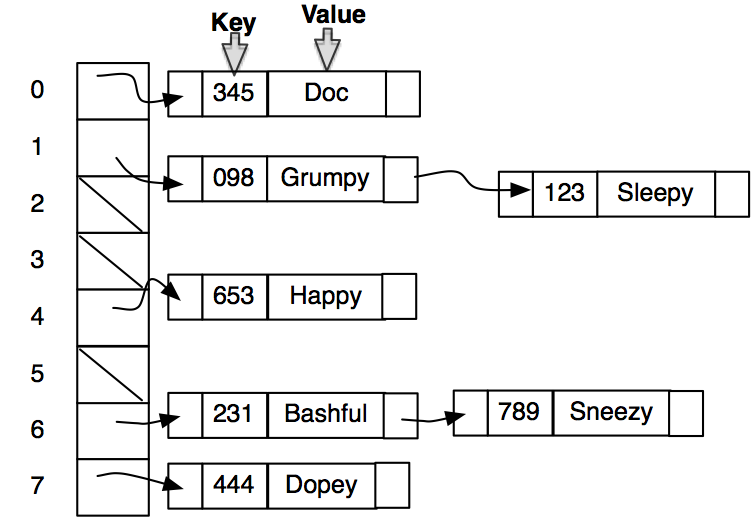
\includegraphics[width=0.5\textwidth]{pictures/Separate_Chaining_0.png}
\caption{Separate Chaining}
\label{fig:sepChain}
\end{figure}




     Separate chaining is often implemented so that none of the data items are stored in the actual hash table.
     Instead the hash table simply houses pointers to the linked lists of data that hash to that location.
     

     Algorithms for separate chaining are easy to construct, as the first step is a simple lookup in an array and the rest of the data structure can be manipulated through linked list operations. If the hash function is good, there will be few collisions and the linked lists will be short.
   
Even though this technique requires more storage space than an open addressing approach, the simplicity and its performance make it a popular choice in hash table design.


\section{Additional Resources}
An excellent hashing tutorial with several animations can be found here:      

       http://research.cs.vt.edu/AVresearch/hashing/

       This tutorial reviews most of what we have learned in this lesson, and        expands the topics somewhat. The animations are excellent and worth exploring.   
       
 \section{Extending Activities}
\begin{itemize}


\item {
Using the division method, calculate hash values for the following set 
       of keys. Calculate once using a table size of 11. Calculate a second 
       time using a table size of 12. do you notice anything about the 
       distributions of the calculated values?



Keys: 54 77 82 13 991 308 68 45 1001 73

}
x
\item {
     The expected search time for Linear probing can be calculated by the following formula:
   
\textbf{ O(1 + 1/(1-loadFactor)) } for a successful search and \textbf{O(1+1/(1-loadFactor)\^2)}  for an unsuccessful search.
     
     Create a chart showing the expected search times (successful and unsuccessful) for the following load factors: .10, .20., .30, .40, .50, .60, .70, .80, .85, .90, .95.
     
     What do these numbers tell you?

}
\item {

     Suppose you have two hash functions H1 and H2  where H1(87) = 10, H2(87) = 3  and  H1(42)=10, H2(42)=7.
     Further suppose that the key 87 is inserted into the table first and then the key of 42.  Show the sequence of table positions tried when using random probing with a constant of 37 and a table size of 11.
     
}
\item {

The expected time for a search using Double hashing can be calculated as shown below:

successful search:  (1/loadfactor)(1+ ln(1/(1-loadfactor))) 

unsuccessful search:  1/(1-loadfactor) 
     
     Calculate a chart of the predicted search times (successful and unsuccessful) for the following load factors: .10, .20., .30, .40, .50, .60, .70, .80, .85, .90, .95.
     
     What do these numbers tell you?
}

\item {

The loadFactor of a hash table using separate chaining to resolve collisions is calculated as the \textbf{number of keys/ the number of chains}
The expected length of search ,  successful or unsuccessful, of Separate Chaining is O(1+loadFactor).  

     
     Calculate 
       a chart of the predicted search times for the following load 
       factors: .10, .20., .30, .40, .50, .60, .70, .80, .85, .90, .95.
     
     What 
       do these numbers tell you?
}

\item {

What factors would you consider when selecting a collision resolution approach for a hash table?

}


\end{itemize}




\chapter {Introduction to Trees}
 A tree is somewhat
similar to a linked list, but, when used properly, can provide very fast
access to specific data elements because data is stored in a sorted
fashion. There are many new terms in this chapter. 

The first section  will familiarize you with the terms and
concepts you will need to understand the algorithms for working with
trees in your programs.

Subsequent sections will help you understand the algorithms
associated with constructing and maintaining a  tree.   It is to your advantage to ensure that you understand the concepts in this chapter before trying to learn about the specific algorithms for binary trees.   Trees are a fundamental data structure in many programming languages and are the base data structure for several other data types including heaps, priority queues,  and search trees.

\section {Simple Rooted Trees}

A tree ADT is similar to a linked list in that it consists of a series
of connected nodes. Unlike a linked list node, a tree node can be
connected to more than two other nodes.

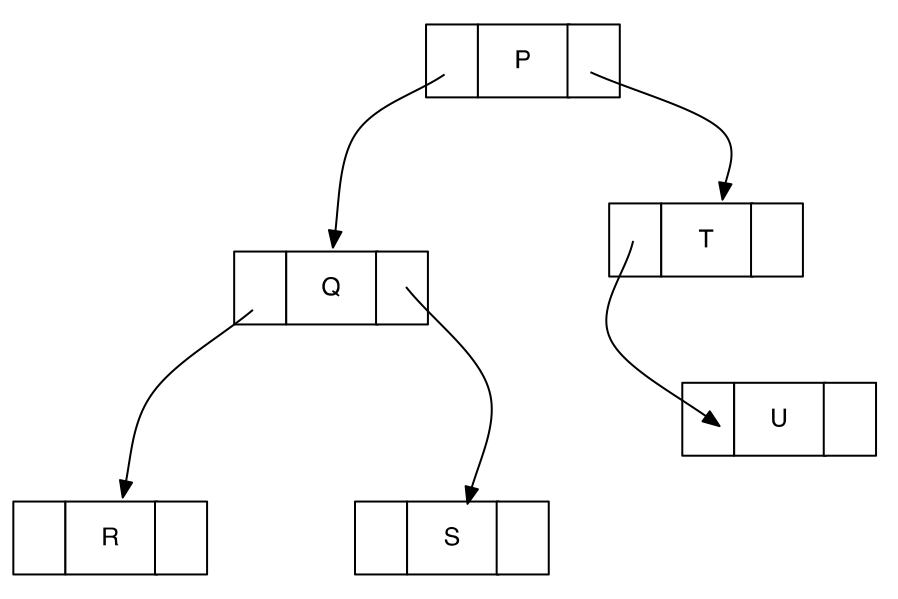
\includegraphics[width=5.80556in]{pictures/image1.png}

Consider the picture above. It shows a tree with six nodes. There are
several terms that you must understand before you can really understand
how a tree ADT works.

\begin{itemize}
\item
  Nodes in trees have relationships to other nodes. We label these
  relationships as \emph{parent}, \emph{child}, \emph{ancestor}.

  \begin{itemize}
  \item
    Node Q in the picture is a child of node P. Node P is the parent of
    nodes Q and T. Node P is the ancestor of node S.
  \item
    Nodes can only have one parent
\end{itemize}
\item
  A tree has a \emph{root node.} In fact a tree can have only one root
  node. The root node has no parent. In the example tree, P is the root
  node.
\item
  Trees have branches. The path between two nodes is called a branch. In
  the example, nodes P and Q have two branches, node T has one branch
  and nodes R, S and U have zero branches.
\item
  Nodes with no branches are known as leaf nodes.
\item
  A tree has a height. The height is the number of nodes in the longest
  path from the root to a leaf. The height of the example tree is 2
  because the longest path is from P to Q to (R or S).  Some algorithms for calculating height count the root node as height one.  For this course we will not count the root node in the height by default.  If the root node is counted it will be explicitly noted.
\item
  Each node in the tree has a level. In the example, nodes Q and T are
  on level 1 because they are children of the root. R, S and U are on
  level 2.
\item
  Trees are recursive: each branch of a tree (each subtree) is also a
  tree.
\end{itemize}
  
  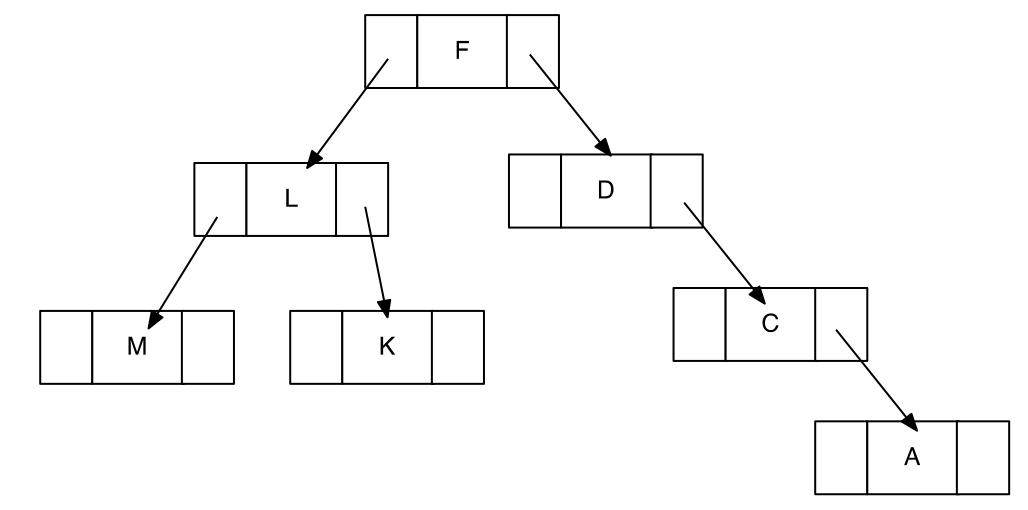
\includegraphics[width=6.00000in]{pictures/image2.png}

Can you answer the following questions about the tree image shown above?  

  How many nodes are in the tree?  (answer 7)

  What is the height of this tree? (answer 3)

  Which node is the root node of the tree? (answer F)

  Which nodes are leaf nodes of the tree? (M, K, A)

  Which node is the parent of node K? (L)

  What is the largest number of branches that any node in this tree has? (2)


 \section {Operations on Trees} 
 \subsection{Tree Insertions}
  When nodes are inserted into a tree, the operation is performed such
  that the nodes are kept in sorted order in the tree. Sorted order can
  be defined any way that the programmer wishes. For example nodes could
  be sorted alphabetically, or they could be sorted by numeric value,
  length, or by some other attribute.
   
   Data entry into a tree is a bit more complicated than it is for linked
  lists. Suppose we were creating a linked list from the following names
  and we wished to keep the list sorted:
  
\begin{itemize}
\item Dopey
\item Sleepy
\item Happy
\item Doc
\item Sneezy
\item Grumpy
\item Bashful
\end{itemize}

We would create the list with the first entry of Dopey and then we'd
insert Sleepy behind it. Happy would get inserted between Dopey and
Sleepy, Doc would be inserted before Dopey, Grumpy would be added after
Dopey and Bashful would be inserted at the head of the list. The
completed list would look something like this:

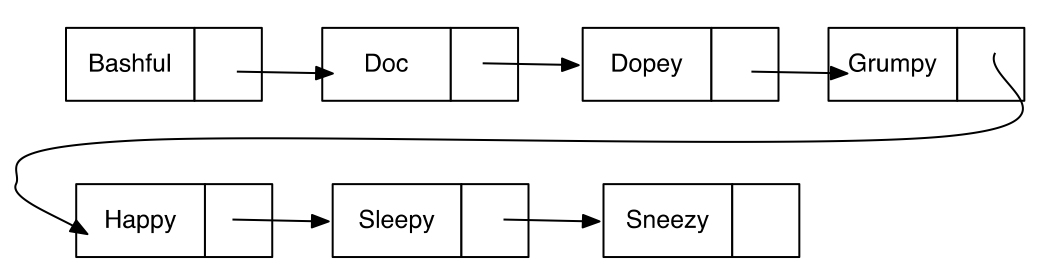
\includegraphics{pictures/image3.png}

However, if we were storing the same data in a tree ADT the
insertion/addition process would be slightly different. Trees use a
compare function to decide if the node to be inserted is larger, or
smaller than the node being compared. Nodes that are larger than the
current node are placed in the right branch, nodes that are smaller than
the current node are placed in the left branch.

So if we started the tree by entering Dopey, the second node, Sleepy,
would be placed in the right branch because Sleepy is `larger'
alphabetically than Dopey. Happy also goes to in the right hand branch
of Dopey, but in the left hand branch of Sleepy because Happy is bigger
than Dopey, but smaller than Sleepy. The finished tree can be seen
below:

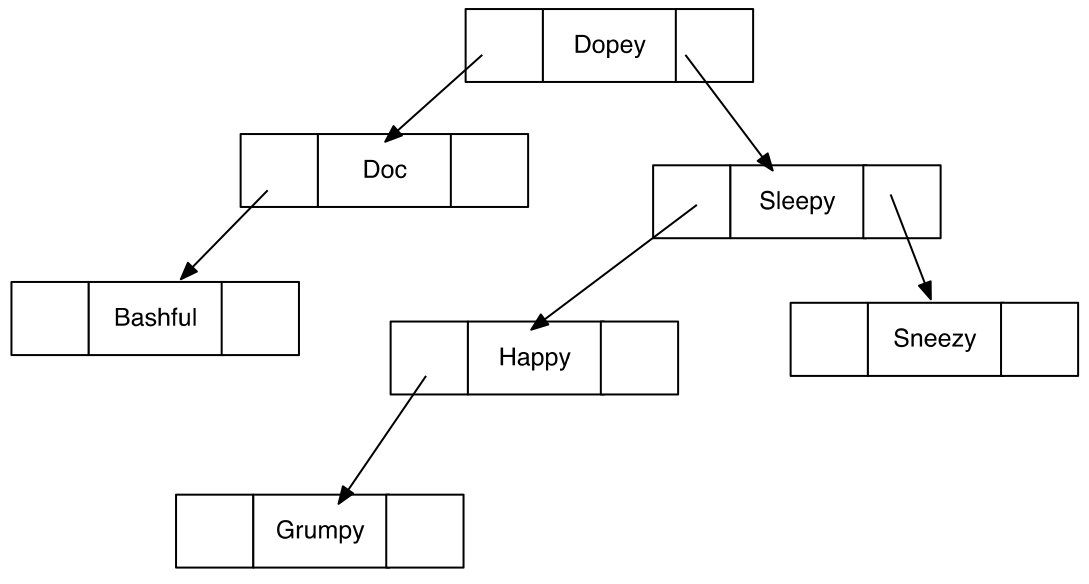
\includegraphics[width=6.00000in]{pictures/image4.png}

\subsection{Removing nodes from a tree}

Because tree nodes can have two children,  the removal of nodes from a tree is more complicated than removing elements from a list.  
Consider the tree shown in the previous section.   If "Doc" were removed from the tree,  the tree could be reconfigured so that Dopey pointed to Bashful and the sorted nature of the tree would not be compromised.

However,  if "Sleepy" were to be removed from the tree, the reconfiguration is much more challenging.  Should  Dopey point to Happy or to Sneezy?  What happens to the other node?    Many tree libraries do not actually delete an element from a tree on removal,  instead the library marks the element "inactive".   It holds its place in the tree, but cannot be returned on searches and cannot be updated.  

We will discuss removing nodes from trees more in subsequent chapters.

\subsection{Tree Traversal}

Nodes in the trees are accessed by traversing the tree. Traversal is
simply a process of walking through the tree by using the pointers that
connect nodes to move from one node to the next. Tree traversal always
starts with the root node of the tree.   An \textbf{iterator} can be used to traverse a tree if the Tree ADT comes with an iterator function.

Imagine that your task was to print all of the values of the nodes in
the tree. What order would they be printed in if you started at the root
node? The answer to that question depends on when you printed each node
and which branches of the tree you followed first. The different
patterns of walking through the tree are traversal schemes.  Two common
schemes are in-order traversal and pre-order traversal.  Both of these traversal algorithms are recursive.



\subsubsection{Pre-order traversal}

Another common traversal technique is Pre-order traversal. The general
idea is the same but the algorithm changes slightly to process the root
node first, before any subtrees are processed. The general algorithm is:

process current node

process left subtree

process right subtree


The pre-order traversal of the tree example shown in section YYYYY is
 Dopey, Doc, Bashful, Sleepy, Happy, Grumpy, Sneezy.
 
 \begin{lstlisting}[showspaces=false, language=make]
 We start at the root (the current node) and print it - Dopey.
   Recurse on the left subtree - printing Doc
         Recurse on Doc's left subtree- printing Bashful
            Bashful has no left subtree
            Bashful has no right subtree
            Return
         Doc has no right subtree
      Recurse on the right subtree - printing Sleepy
         Recurse on Sleepy's left subtree - printing Happy
            Recurse on Happy's left subtree printing Grumpy
               Grumpy has no left subtree
               Grumpy has no right subtree
               return
             Happy has no right subtree
             Return
           Recurse on Sleepy's right subtree printing Sneezy
                 Sneezy has no left subtree
                 Sneezy has no right subtree
                 Return
\end{lstlisting}		     		
				
\subsubsection{In-order traversal}

An in-order traversal visits each node in sort order and processes the
node as it is visited. For example, if the nodes in the example tree
were traversed in order, and the processing action was to print the
value, the result would be an alphabetized list of names.

To conduct an in-order traversal, the algorithm must move to the
smallest value in the tree (which will be the left most leaf), process
that leaf, move to its parent, process the parent, move to the right
branch and repeat.

For each tree (and subtree) the algorithm is:

\begin{itemize}
\item
  process left subtree
\item
  process root
\item
  process right subtree
\end{itemize}

The key difference between pre-order and in-order traversal is when the root node is processed.  The in-order traversal for the example tree  is  shown below:

\begin {lstlisting}
Start at the root but do not process it
Recurse to process the left subtree.
	This means we must move to Doc but do not process it because it is the root
		Recurse to process the left subtree
			This means we must move to Bashful but do not process it
			Bashful has no left subtree
			process the root and print Bashful
			Bashful has no right subtree so we return
		Process the root and print Doc
		Doc has no right subtree so we return
	process the root and print Dopey
	Recurse to Process the right subtree
		This means we must move to Sleepy
			Recurse to process the left subtree
			This means we must move to Happy
			Recurse to process the left subtree
				This means we must move to Grumpy
				Grumpy has no left subtree
				process the root and print Grumpy
				Grumpy has no right subtree so we return
			process the root and print Happy
			Happy has no right subtree so we return
		Process the root and print Sleepy
		Recurse to Process the right subtree
			This means we move to Sneezy
			Sneezy has no left subtree
			process the root and print Sneezy
			Sneezy has no right subtree so we return
			
			done.
\end{lstlisting}





\section{Binary Trees}

While a tree ADT can have any number of branches theoretically, often we
limit the number of branches. A binary tree (one with nodes that can
have at most two branches ) is a very common ADT. 

\subsection {C Structure for Binary Tree ADT}

As with any ADT, the Binary tree needs a structure to hold the pointers
to its connected nodes and to hold a pointer to the data. A binary tree
node is usually labeled with pointers called `left' and `right' to
denote the child nodes.

\begin{lstlisting}
struct BinTreeNode
{
	void * data
	struct BinTreeNode * left
	struct BinTreeNode * right
	Tree * myTree;  //not required, but  useful for getting the function pointers
};

struct BinTree
{
	int compare function
	void destroy function
	Struct BinTreeNode * root;
};

typedef Struct BinTree Tree;
\end{lstlisting}

Because the Binary Tree ADT stores \emph{void * } data,  the user of the tree ADT must supply a function pointer for
the destruction of the data and clean up of memory as well as for comparing data elements to determine the position of the data in the tree.

  The Tree ADT
must guarantee that all nodes that are removed, either individually
or when the tree is destroyed, will be properly removed from memory
using the supplied function. 

Also, because data in a binary tree is kept
in sorted order, the user of the ADT must supply a function pointer to a
compare operation that can compare the values of two data items. (If you
are fuzzy about function pointers, go back to the function pointer
review).

Binary tree operations can be divided into two sets. The first set are
sometimes called wrapper operations  These are the operations that the
user of the ADT will call.  Wrapper functions typically take the Tree Struct as a parameter, possibly along with other paramters.

The second set of operations are the helper
operations. These are the operations that actually do the work of
setting up, manipulating, and keeping track of the tree.  The helper operations typically take the root node of the tree as a parameter ( the \textbf{root} member variable of the Tree struct) along with other paramters.  Often helper operations for trees are recursive.
Below you can find a list of some common wrapper and helper operations on binary trees.

\begin{lstlisting}

//ADT Wrapper Operations

createBinaryTree( compare function pointer, destroy function pointer):BinTree
destroyBinaryTree(BinTree *): void *
addToTree (void * data)
removeFromTree(void * data): Boolean
findInTree(void * data):void *

//Helper Operations

TreeNode * insert(TreeNode * root, TreeDataType data);
TreeNode * delete(TreeNode * root, TreeDataType data);
bool isEmpty(TreeNode * root);
bool hasTwoChildren(TreeNode * root);
int compare (TreeDataType data1, TreeDataType data2);
TreeNode * findMinimum(TreeNode * root);
void printInOrder(TreeNode * root);
\end{lstlisting}

In addition to wrappers and helpers, most tree ADTs provide operations
that will traverse the tree and do something during the traversal. The
elegant way to provide node-processing functionality is to provide
traversal operations that accept a function pointer. The function is
executed once for every node in the tree.

Lets start our exploration of binary trees by looking at the helper
functions starting with insertion. We'll ignore the data types and
function pointers for now, but will return to them towards the end of
this chapter.

\subsection{Recursive Helper Functions}
\subsubsection{Insertion}

Insertion into a tree has three possible cases:

\begin{enumerate}
\item
  The tree has no nodes, and the value will be inserted as the root node
\item
  The value to be inserted is larger than the value at the root, and
  will be inserted in the right subtree of the root node.
\item
  The value to be inserted is less than the value of the root, and will
  be inserted into the left subtree of the root node.
\end{enumerate}

Cases 2 and 3 result in a recursive call to the insertion operation.

\begin{lstlisting}
insert(TreeNode * root, TreeDataType data, funcPointer to compare operation): TreeNode *

if (the root node is empty)
{
	allocate memory for a TreeNode and assign it to temp
	temp-\textgreater{} data = data
	temp -\textgreater{} left = NULL;
	temp -\textgreater{} right = NULL;
	return temp;
}
if(compareFunction(root-\textgreater{}data, data) shows root data is smaller)
{
	/*recursively call insert on right subtree*/
	root-\textgreater{}right = insert(root-\textgreater{}right,data, comparePointer)
}
else if(compareFunction(root-\textgreater{}data, data) shows root data is larger)
{
	/*recursively call insert on left subtree */
	root-\textgreater{}left =insert(root-\textgreater{}left,data,comparePointer);
}
/* Else there is nothing to do as the data is already in the tree. */
return root;
}
\end{lstlisting}


Because a binary tree is stored in sorted order, insertions have to be
done by comparing the data to be inserted to the data stored at the
current node. Insertions are always done at a leaf node. By supplying a
function pointer for the comparison operator, a tree ADT can
successfully insert any type of data.

Here is a visual look at the insert operation.

Suppose we wanted to insert 17 into the tree shown.

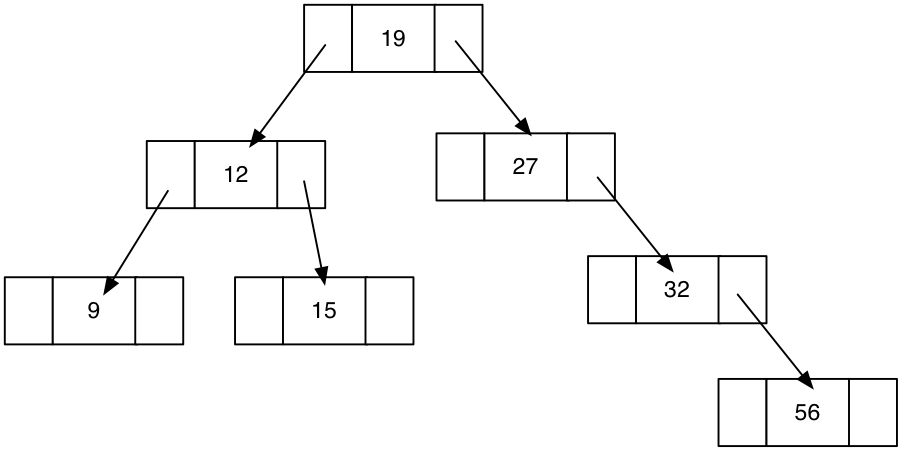
\includegraphics[width=6.00000in]{pictures/bintree1.png}

We first compare 17 to the value at the root node (19). Since 17 is
less than 19, and in this binary tree we are storing the smallest values in the left subtree,  we recursively call the insert procedure on the left
subtree of 19.

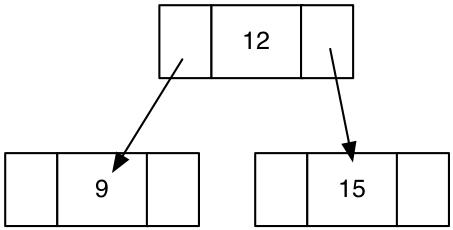
\includegraphics[width=3.01389in]{pictures/bintree2.png}

We compare 17 to the root node of the subtree. 17 is greater than 12, so
we recursively call the insert procedure the right subtree of 17- which is the node containing 15.


17 is larger than 15, so we recursively call the insert procedure on the
right subtree of 15. That subtree is a NULL tree, which activates the
base case of the recursive algorithm.

A node is made for 17, the pointer to it is returned as the recursion
unwinds.

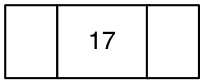
\includegraphics[width=1.34722in]{pictures/bintree3.png}

On the way back up, the tree reassembles each level.

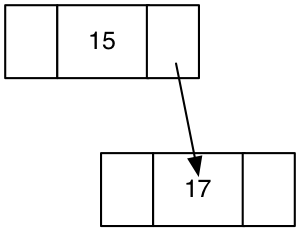
\includegraphics[width=1.98611in]{pictures/bintree4.png}

Then

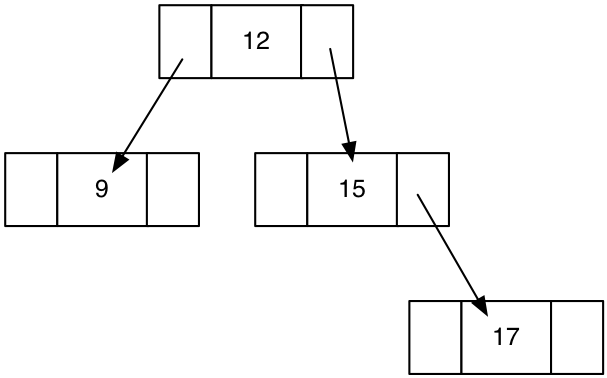
\includegraphics[width=3.65278in]{pictures/bintree5.png}

and finally back to the entire tree.

\subsubsection{Deletion}

Deletion from a binary tree is a bit trickier because you have to be
careful to keep the tree in the proper order.

There are three cases to consider when deleting a node from a binary
tree:

\begin{enumerate}
\def\labelenumi{\arabic{enumi})}
\item
  the node has no children
\item
  the node has only one child (left or right branch)
\item
  the node has two children
\end{enumerate}


The first case is easy. If the node to be deleted has no children (i.e.
it is a leaf node) it can be deleted and the appropriate branch of its
parent set to NULL.

In the second case, If the node to be deleted has a right branch child,
then the deleted node's parent can be set to point at the child and the
tree will remain in the correct order.

Suppose we needed to delete 32 from the subtree below. We could simply
remove 32 and set 27 to point at 56 and the properties of the binary
tree would not have changed.

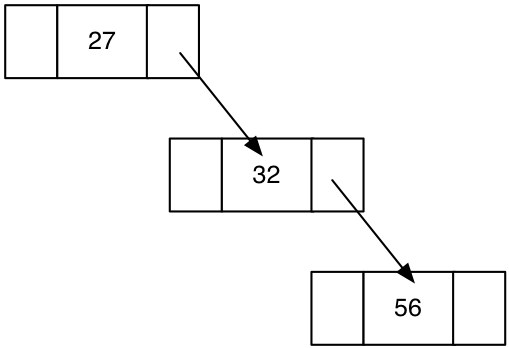
\includegraphics[width=3.38889in]{pictures/bintree6.png}

If a node has a left child only, the same process can be used to remove
the node. Attach the nodes left child to the node's parent and the tree
structure will still be valid.

The more complicated case arises when the node to be deleted has two
children.

Suppose that we want to delete node 12 from this tree. We can't simply
remove 12 and put either one of its children in its place, because we
would lose part of a subtree. If 15 replaced 12, there would be no place
to reattach 9 and a similar problem exists if 9 were used to replace 12.

%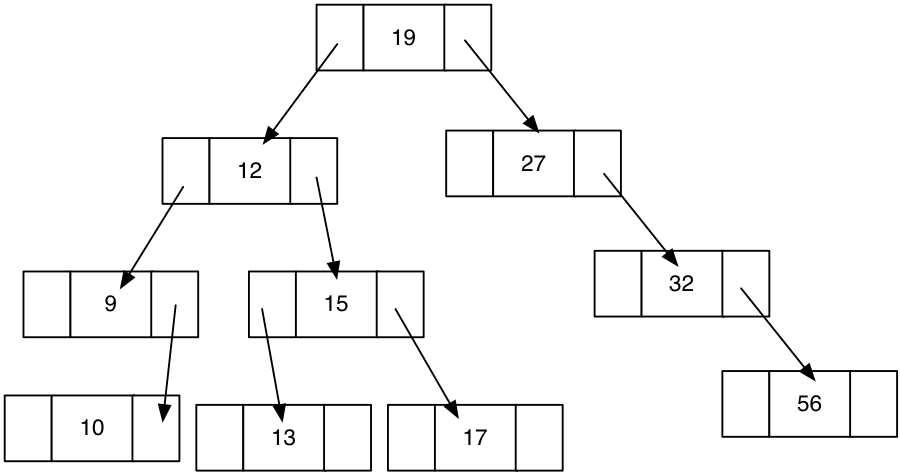
\includegraphics{pictures/bintree7.png}

The problem is solved by remembering that the right subtree always
contains values that are larger than the node, and the left subtree
contains values that are greater. So, for any node, the smallest value
in the left subtree will be a node that has a value slightly larger
than the node being removed, but smaller than all the other nodes in the
subtree. That node will also be a leaf node in the tree.

The algorithm is this:

\begin{itemize}
\item
  find the minimum value in the right subtree of the node to be deleted
\item
  copy that value into the node to be deleted (temporarily making a
  duplicate node)
\item
  recursively call delete on the right subtree -- for the value we just
  copied in. This will activate the base case of the node having no
  children and will remove the node
\end{itemize}

In the case of the previous example, we would copy the value 13 into the
node that presently holds 12, and then call delete (13) on the subtree
rooted at 15. The node at 13 will be removed and the tree will look like
this:

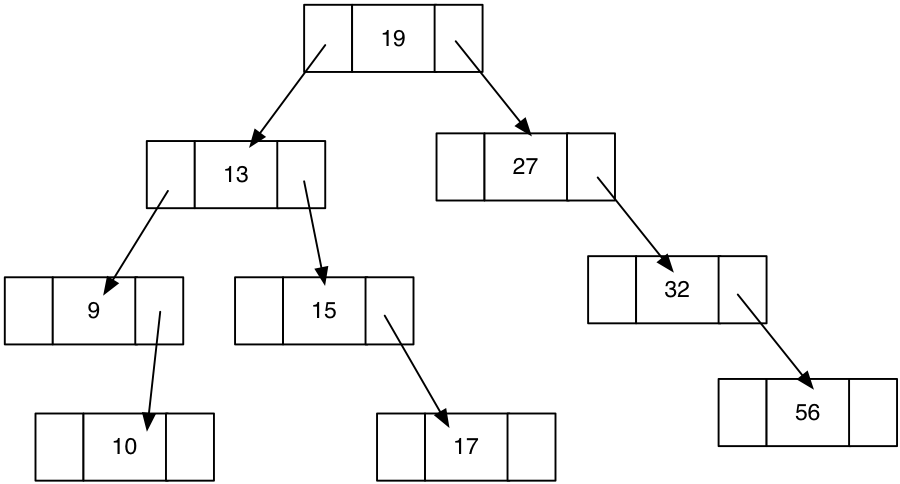
\includegraphics[width=6.00000in]{pictures/bintree8.png}

\begin{lstlisting}
TreeNode * delete(TreeNode * root, TreeDataType data, compareFP,destroyNodeFP):TreeNode

TreeNode * temp;
TreeDataType removedData;

if the root is empty
	we have a problem and should clean up and exit gracefully
else if (compareFP(root-\textgreater{}data, data) shows that the root data is larger)
{
	root-\textgreater{}left = delete(root-\textgreater{}left, data, compareFP, destroyNodeFP);
}
else if (compareFP(root-\textgreater{}data, data) shows that the searched for data is larger)
{
root-\textgreater{}right = delete(root-\textgreater{}right,data,compareFP, destroyNodeFP);
}
else /*the comparison is equal and we can delete the node we've found */
{
	if (the root node has two children) /*replace this node with the smallest element in right subtree */
	{
		temp = findMinimum(root-\textgreater{}right)
		removedData = root-\textgreater{}data
		destroyFP(root-\textgreater{}data) /*now call destroy function on that data */
		root-\textgreater{}data = temp-\textgreater{}data
		root-\textgreater{}right = delete(root-\textgreater{}right,
		temp-\textgreater{}data,compareFP, destroyFP)
	}

	else  /*this node has zero or one child*/
	{
		temp = root;
		if (root-\textgreater{}left == NULL) /* we have no left child */
		{
			root = root-\textgreater{}right;
		}

		else if (root-\textgreater{}right == NULL) /*we have no right child */
		{
			root = root-\textgreater{}left;

		}
	}
	/*either we've rejoined the subtree, or we're about to delete a leaf node*/

	destroyFP(temp-\textgreater{}data);/*call destroy function on temp-\textgreater{}data */
	free(temp);

}
\end{lstlisting}
\subsection{Wrapper functions}

The wrapper functions for a Tree ADT provide the interface that the user
of the ADT interacts with.
The wrapper functions are not recursive rather, they call the recursive
functions when appropriate.

\begin{itemize}
\item {createBinaryTree( compareFP, destroyNodeFP)): Tree *

createTree is used to initialize a tree and to set up the function
pointers for the data type that the tree will be storing. When function
pointers are used, and data is cast to a void pointer, the same compiled
tree library can be used to hold any kind of data.
}
\item {destroyBinTree(Tree * toDie)

destroyBinTree is called when the tree must be released. The destroy
tree function will recursively destroy all the tree nodes AND all of the
data elements (using the supplied function pointer).
}

\item {addToTree(Tree, void * )

addToTree inserts a value into the tree by calling the recursive insert function.
}

\item {removeFromTree(Tree*, void *)

removeFromTree searches for the data provided in the parameter and, if found, removes that data from the tree.  Remove from tree should also free the memory allocated for the node.  It is a design choice as to whether removeFromTree also frees the memory for the data.

}

\item {findInTree(Tree *, void *):Boolean 

findInTree returns true(1) if the data is found, false(0) if not.
}

\end{itemize}

The wrapper functions are usually not complicated and mostly call the recursive helper function for the
appropriate operation, passing in the function pointers and parameters to the operation as necessary. See the given code
for addToTree for an example.

\begin{lstlisting}
void addToTree (Tree* theTree, void * data)
{
	theTree-\textgreater{}root = insert(theTree-\textgreater{}root, data,theTree-\textgreater{}compare);
}

\end{lstlisting}


\subsubsection{Traversals}

Another common set of functions for trees are traversal algorithms.  A traversal algorithm can also be used to create an \textbf{iterator} for a tree. Traversal algorithms were introduced in the introductory section on single-rooted trees.  In addition to the  in-order and pre-order traversals explored in that section,  a tree traversal can be written to be in post-order (the root is processed after the subtrees- left subtree, right subtree, root)  or in level-order where the root is processed,  then all of the root's immediate children,   then all of the root's grandchildren,  then all of the root's great grand children, etc.  A level-order traversal is also known as a breadth-first traversal.

A recursive algorithm for a level-order traversal of a tree is shown below.   

\begin{lstlisting}
for ( the height of the tree)
{
    processLevel(TreeNode * root, height)
}

void processLevel( TreeNode * currentNode, int level )
{
    if ( currentNode  is NULL)
        return;
    if (level == 1)
        process  currentNode->data //processing could be printing or something else
    else if (level > 1)
    {
        processLevel(currentNode->left, level-1)
        processLevel(currentNode->right, level-1)
    }
\end{lstlisting}



Often a traversal function will take a function pointer as an argument
and will apply that function to the data in each node of the tree. For
example, you could write a function that printed a node value, and then
combine that function with a traversal function to print the tree in a
variety of orders. 

The print function is data dependent,but the traversal function is not.  
For example, a function to print  integer data might look like this:

\begin{lstlisting}
void printIntNode(void * data)
{
	printf("\%d ", data);
}

\end{lstlisting}

where a function to print values from a tree that was storing strings
might look like this

\begin{lstlisting}
void printStringNode(void * data)
{
	printf("\%s ", data);

}
\end{lstlisting}

A traversal algorithm could be called, sending it the print function,
and any type of data could be successfully printed. For example.
\begin{lstlisting}
printInOrder(myTree-\textgreater root, \&printIntNode);

//or

printInOrder(myTree-\textgreater root, \&printStringNode);
\end{lstlisting}

The key to remember that the user of
the ADT is the one who defines the data stored by the ADT and the
operations to compare, destroy, and manipulate that data. The tree ADT
simply stores the data and performs the requested operations when given
pointers to those operations.


\section{Types of Binary Trees}

A binary tree is \textbf{full} if every node in the tree has zero or two children.     A full binary tree has the property where the number of leaf nodes (L) is equal to the number of internal nodes (I) + 1.    If you are curious about the proof of this propertly see
 \url{http://www.geeksforgeeks.org/handshaking-lemma-and-interesting-tree-properties/}
  \begin{figure}[H]
\centering
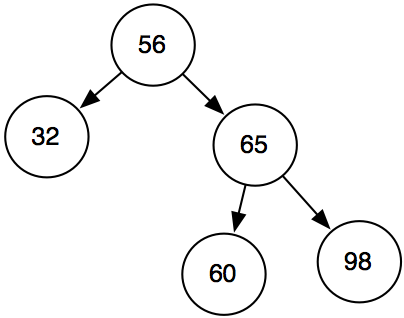
\includegraphics{pictures/fullTree.png}
\label{fig:fullTree}
\caption{A full binary tree}
\end{figure}

A binary tree is \textbf{complete} if all the levels of the tree are full excepting possibly the last level.   The last level must have all the nodes as far to the left hand side of the tree as possible.    A complete binary tree is used in the implementation of a \textbf{heap}.

  \begin{figure}[H]
\centering
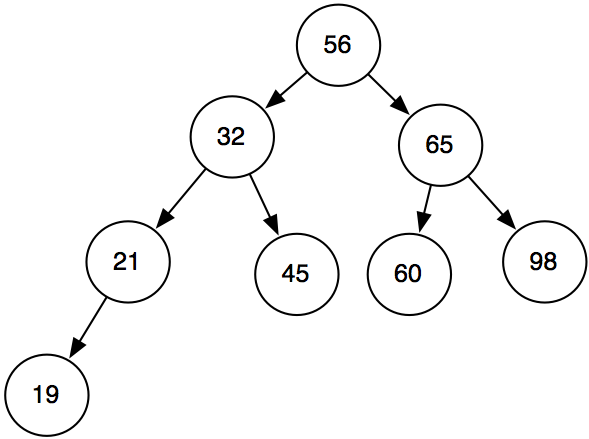
\includegraphics{pictures/completeTree.png}
\label{fig:fullTree}
\caption{A complete binary tree.  All of the levels in the tree have two child nodes except for the last level.  The child nodes in the 
last level are as far left as possible.}
\end{figure}

A \textbf{perfect} Binary tree is one in which all internal nodes have two children.   The leaf nodes of a perfect binary tree are all at the same level.
The number of nodes in a perfect binary tree is $2^h-1$ where h is the height of the binary tree.  

  \begin{figure}[H]
\centering
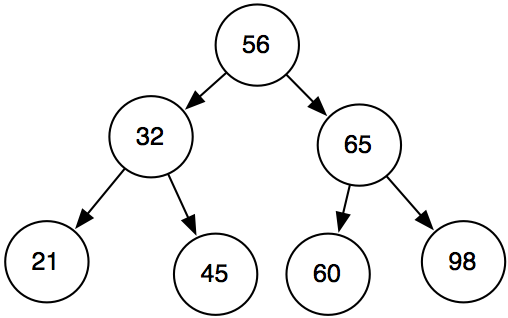
\includegraphics{pictures/perfectTree.png}
\label{fig:fullTree}
\caption{A full binary tree}
\end{figure}

 

\section{Extending Activities}

\begin{itemize}


	\item {The order that nodes are inserted into a tree can greatly affect the
	structure of the tree. Draw the binary tree that is constructed by adding the
	seven names in the following order:
	
	\begin{itemize}
	\item
	  Sleepy
	\item
	  Bashful
	\item
	  Doc
	\item
	  Dopey
	\item
	  Sneezy
	\item
	  Happy
	\item
	  Grumpy
	\end{itemize}
	}



\item{ Trace the algorithms for level-order traversal using a hand
drawn tree.  What order are the nodes of the tree printed in?  Can you tweak the algorithm to reverse the order?
}
	
	
	
\item{ One of the most frequent uses of a binary tree is as a
search tree. The object is to search through the data to find out if a
particular element is part of the data. Write a recursive find procdure
for a binary tree. Start with the root node of the tree. Your procedure
can be in c or in pseudocode. Be sure to pass in the compare function
pointer.

}



	\item{
	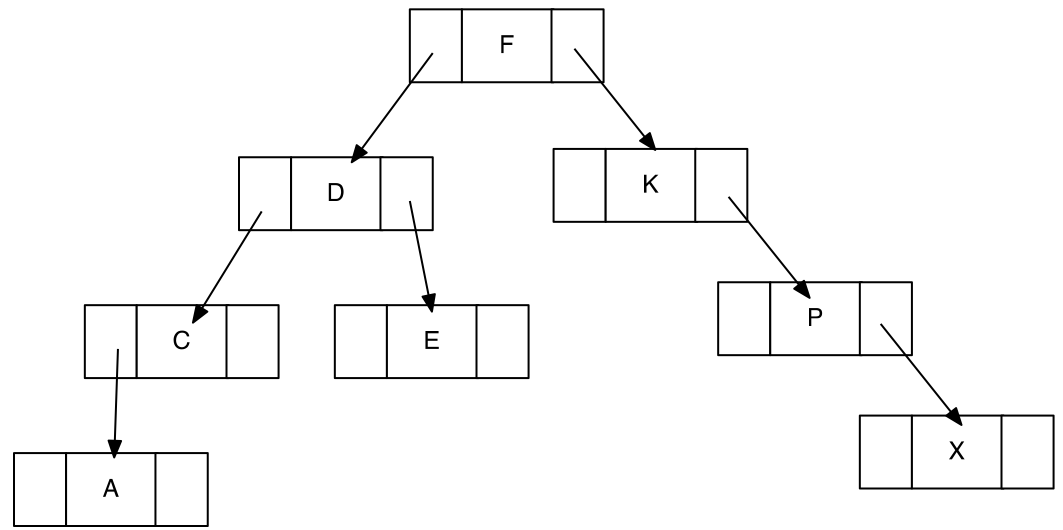
\includegraphics[width=6.00000in]{pictures/image5.png}
	
	Give the in-order traversal of the tree shown above.
	
	Give the pre-order traversal of the tree.
	}

\item Write the pseudocode or c code for a compare operator. A
compare operator must return three distinct values, one for when the
first parameter is larger, one for when the second parameter is larger,
and one for when the two parameters are equal. The convention is to use
1, 0, and -1 for the three values. Zero for equal values, 1 for the
first string being larger, -1 for the second. 


\item The delete operation relies on a recursive function to
find the minimum value in a subtree. The minimum value will always be
the leftmost leaf of the subtree. Write the findMinimum function (in
pseudocode or in C).

\end{itemize}



 
\chapter{Heaps}
\section{Introduction}
A heap is a special kind of complete binary tree.  The key property of a heap is that  the target element (the minimum or the maximum) is always stored at the root of the heap.   This is done by reordering the nodes to ensure that the property is true.   A heap can be one of two types, a max heap where the parent node is greater than its children, or a min heap where the parent node is smaller than its children.

To be a valid heap, every element has to follow the heap rule. For max heaps the rule is: \begin{equation}value(parent) \geq value(child)\end{equation}   and for a min heap the rule is: \begin{equation}value(parent) \leq value(child)\end{equation}

A heap is considered to be a partially ordered data structure because the elements within any given level have no defined ordering.  Heaps are commonly used as the implementation for a priority queue.

\begin{figure}[H]
\centering
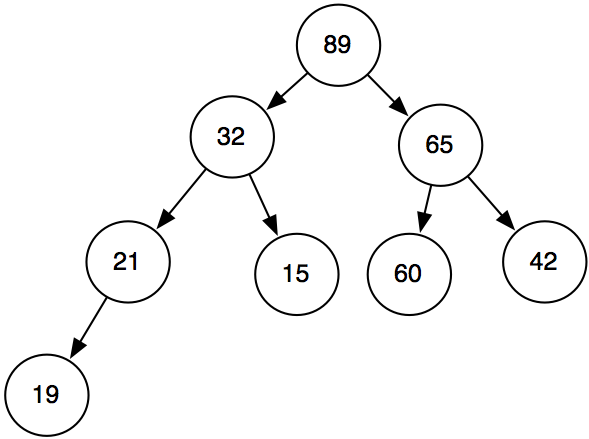
\includegraphics{pictures/maxheap.png}
\label{fig:maxheap}
\caption{A max heap.  Notice that the sibling nodes have no ordering within the level}
\end{figure}


\section{Operations}
A heap should provide the functionality to insert, delete, and retrieve the min/max value.    Additionally the heap must provide the standard data structure operations of create, destroy and isEmpty.   A robust heap library should allow the library user to choose between min or max heap capabilities when the heap is created.  The minimum set of operations is shown below.  

\begin{itemize}
\item insert
\item delete
\item findMinorMax
\item isEmpty
\item create
\item destroy
\end{itemize}

The Heap ADT requires the same abstraction with void * pointers,   operations to create nodes,  and function pointers to compare, delete and print data as the previous ADTs we have studied.     The create, destroy, and isEmpty functions are very similar to the same functions for other ADTs and are not explained in detail here.

The insert and delete functions for a heap are the most complicated operations.   

\subsection{Heap Insert}

A heap is a specialized version of a complete tree.  This means that all insertions must occur at the left-most side of the bottom level of the tree in order to maintain the property of completeness.   The algorithm for adding an element to a heap follows:
\begin{lstlisting}
insert(Heap * heap, void * data)
{
    create a node from the data
    locate the next position in the heap (the left most position with no node)
    add the new node to the located position
    reheapify the heap to maintain the heap property
}
\end{lstlisting}

The process of reheapification consists of swapping elements until the heap property is satisfied or until the root of the heap is reached.  The pseudocode for reheapification is shown below.

\begin{lstlisting}
reheapify(Heap * heap, Node * newNode)
{
     parentNode = get parent node of newNode
     while(newNode->data is greater than parentNode->data  //or less than for a min heap
     {
     	swap positions of newNode and Parent Node
     	parentNode = get parent node of newNode (has changed because of the swap)
     }
}
 \end{lstlisting}
 
\subsection{Heap Delete}
 
 The most common way to delete elements from a heap is to remove the value at the root node as part of the the findMinorMax operation.
 To remove the root node,  you find the left-most leaf of the heap,  replace the root node with that node, and then reheapify downwards until the heap property is satisfied.
 
 \begin{lstlisting}
 void * findAndDeleteRoot(Heap * heap)
 {
 	tempNode = heap->rootNode
 	heap->rootNode = the node in the "last" position in the tree //the leftmost, bottom node
 	outOfPlacePtr = heap->rootNode  // keep track of the node that you're moving into place
 	remove the node in the last position //after copying it into the root
 	while ( outOfPlacePtr->data is less than either left or right child)  //or greater than for a min heap
 	{
 		swap outOfPlacePtr and child with greatest value
 	}
 	return tempNode->data
 }
 \end{lstlisting}
 
 The delete process for the root node can be used to delete any node in the heap.   The node to be deleted is the root node of a subtree,  and the delete algorithm can be applied to the subtree instead of the entire heap.
 
\section{Array Implementation of a Heap}

Heaps can be implemented using a Binary Tree ADT.  However,  the property that a heap is a complete binary tree allows a heap to be implemented using an array.  The array implementation removes the need for pointers as the positions of the child nodes can be easily calculated.   The first empty position in the array is the next position to be filled.

\begin{figure}[H]
\centering
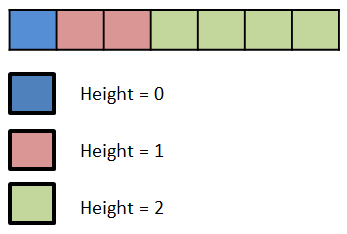
\includegraphics{pictures/heap0.png}
\label{fig:heap0}
\end{figure}

The array is organized so index 0 is height 0, height 1 is indexes 1-2, height 2 is indexes 2-5 and so on.   The swaps necessary for inserting or deleting elements can be accomplished simply by calculating the appropriate array index.

\subsection{Adding Elements}

Adding an element to a heap has a worst case complexity of O(height) or O(log(N)), since there is a maximum of 1 swap per level of the heap.
The algorithm for inserting elements does not change when an array is used for implementation.  Only the implementation details change.   Consider the following example where 10, 23, 3, 32, 17 and 5 are added to a max heap.

We begin by adding 10 to an empty heap.

\begin{figure}[H]
\centering
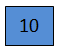
\includegraphics{pictures/heap1.png}
\label{fig:heap1}
\end{figure}

\begin{figure}[H]
\centering
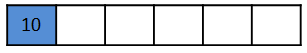
\includegraphics{pictures/heap1a.png}
\label{fig:heap1a}
\end{figure}

10 is added as the root of the heap at position 0 in the array.   It is the first level of the binary tree.  
We then add 23 to the heap.

\begin{figure}[H]
\centering
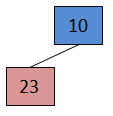
\includegraphics{pictures/heap2.png}
\label{fig:heap2}
\end{figure}

\begin{figure}[H]
\centering
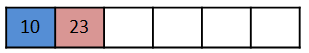
\includegraphics{pictures/heap2a.png}
\label{fig:heap2a}
\end{figure}

First, 23 is added as 10's child.  It is placed in the first empty left-most position in the tree, which is also the first empty position in the array.
Because 23 is greater than 10,  the heap must be reheapified.  

\begin{figure}[H]
\centering
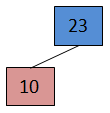
\includegraphics{pictures/heap3.png}
\label{fig:heap3}
\end{figure}

\begin{figure}[H]
\centering
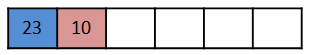
\includegraphics{pictures/heap3a.png}
\label{fig:heap3a}
\end{figure}

23 is compared to its parent value (10).  23 is larger so the two values are swapped and 23 is the new root of the heap.  10 is the child of 23.   We then add 3 to the heap.   

\begin{figure}[H]
\centering
\includegraphics{pictures/heap4.png}
\label{fig:heap4}
\end{figure}

\begin{figure}[H]
\centering
\includegraphics{pictures/heap4a.png}
\label{fig:heap4a}
\end{figure}

3 is added as the second child of 23.   It is added in position 2 of the array.   3 is compared to the value of its parent (23).  3 is smaller than its parent value so no swap is needed.   We then add 32 to the heap.

\begin{figure}[H]
\centering
\includegraphics{pictures/heap5.png}
\label{fig:heap5}
\end{figure}

\begin{figure}[H]
\centering
\includegraphics{pictures/heap5a.png}
\label{fig:heap5a}
\end{figure}

32 is added at the next, left-most position in the heap (the first empty position in the array).  32 is compared with its parent value (10).  32 is larger than 10 so the two values must be swapped.

\begin{figure}[H]
\centering
\includegraphics{pictures/heap6.png}
\label{fig:heap6}
\end{figure}

\begin{figure}[H]
\centering
\includegraphics{pictures/heap6a.png}
\label{fig:heap6a}
\end{figure}

32 iis not the root of the heap, so we again compare 32  with its parent value (23).   32 is larger than 23, so a swap must be made.

\begin{figure}[H]
\centering
\includegraphics{pictures/heap7.png}
\label{fig:heap7}
\end{figure}

\begin{figure}[H]
\centering
\includegraphics{pictures/heap7a.png}
\label{fig:heap7a}
\end{figure}

32 is the new root of the heap so no further comparisons are necessary.   We then add 17 to the heap.

\begin{figure}[H]
\centering
\includegraphics{pictures/heap8.png}
\label{fig:heap8}
\end{figure}

\begin{figure}[H]
\centering
\includegraphics{pictures/heap8a.png}
\label{fig:heap8a}
\end{figure}

17 is added as a child of 23 to the first, left-most empty position in the tree.  17 is compared to the value of its parent(23).  17 is smaller than its parent value so no swap is required.   We then add 5 to the heap.

\begin{figure}[H]
\centering
\includegraphics{pictures/heap9.png}
\label{fig:heap9}
\end{figure}

\begin{figure}[H]
\centering
\includegraphics{pictures/heap9a.png}
\label{fig:heap9a}
\end{figure}

5 is added to the next position in the heap, as the first child of 3.    5 is compared to its parent value (3).  5 is larger than three so the two values must be swapped.

\begin{figure}[H]
\centering
\includegraphics{pictures/heap10.png}
\label{fig:heap10}
\end{figure}

\begin{figure}[H]
\centering
\includegraphics{pictures/heap10a.png}
\label{fig:heap10a}
\end{figure}

Finally 5 is compared to its new parent (32).  5 is smaller than 32 so no swap is necessary.

It can be seen that the final array representation is not fully sorted, and not fully segregated by value ranges (5 has a height of 1, higher than 10 and 17).   Nonetheless the heap rule holds and the partial ordering of the heap can easily be maintained by swaps.



\subsection{Removing Elements}

Elements of a heap are generally removed from the root, or the largest/smallest element in the structure. The root is then filled with the most recent added element , and the heap is resorted by swapping with the larger child until it satisfies the heap property.   If it is necessary to remove an interior item from a heap,  the subtree rooted in the item to be removed is handled in the same fashion as the entire heap.


Removing an element will always result in a complete tree because only leaf nodes are actually removed after the value is swapped in to a new spot.

The complexity of a deletion is O(height) or O(log(N)) since there is a maximum of 1 swap necessary per height.

\begin{figure}[H]
\centering
\includegraphics{pictures/heap11.png}
\label{fig:heap11}
\caption{The Starting Heap}
\end{figure}

\begin{figure}[H]
\centering
\includegraphics{pictures/heap12.png}
\label{fig:heap12}
\end{figure}

The root is removed, leaving an empty spot in the heap.

\begin{figure}[H]
\centering
\includegraphics{pictures/heap13.png}
\label{fig:heap13}
\end{figure}

The most recently added element is copied to the root position.   The most recently added node is deleted.  The new root node(3) is compared to both of its child nodes (23, and 5).   3 is less than at least one of its children so it must be swapped.   
The heap does not follow the heap rule, a sort must be done.

\begin{figure}[H]
\centering
\includegraphics{pictures/heap14.png}
\label{fig:heap14}
\end{figure}

3 is swapped with the larger child, 23.  3 is now compared with its new children (10 and 17).    3 is smaller than at least one child, therefor the heap still does not satisfy the heap property.  Another swap must be performed.

\begin{figure}[H]
\centering
\includegraphics{pictures/heap15.png}
\label{fig:heap15}
\end{figure}

3 is swapped with the larger child, 17. The heap property is now satisfied.


\section{Extending Activities}

\begin{itemize}
\item Develop a formula to calculate the position of a parent node in an array-implementation of a heap.  The only input information to the formula is the position of the current node.
\item Create the C struct for a binary-tree based heap.  Your struct should have members for the heap,  the last added element, the next position, and function pointers to manipulate void* data.
\item Heaps do not have to be binary trees.   Many variations of heaps are possible.   Use internet resources to learn about one of the following different types of heaps:  skew heaps, binomial heap, or leftist heap.   Write the pseudocode for insert and delete operations for the type of heap you chose.
\item The complexity of insert and delete for a binary heap is O(log(N)).   Why is that?  Create a written explanation, chart, or diagram that explains why log(N) is the complexity for those operations.

\end{itemize}

%to be inserted into data structures textbook in the heaps chapter, after the heap's main functionality

\chapter{Priority Queue}

A priority queue differs from a normal queue because the elements do not follow a FIFO order. Instead elements are removed by the queue in order of priority, with the highest priority elements leaving first. If many items enter a priority queue at the same time the highest priority will be served first followed by the next lowest priority etc. The process gets more interesting when new items are being added sequentially. 

\section{Uses}
A priority queue is useful in any situation where scheduling must occur and the items being scheduled are not handled on a first come first served basis.   For example,  A priority queue would be ideal in an IT department where a lot of people are having a variety of issues. Some issues require immediate attention whereas some others can be put off for a short period of time.  If an entire network was to collapse and join the end of IT ticket queue, behind a long list of lost or forgotten user passwords you'd want the network issue to be fixed first since it effects a lot more people. After the network issue is fixed the less urgent issues will be fixed in the same order as before.

Priority queues are useful in scheduling jobs for execution on computing systems.   Most operating systems use some kind of priority mechanism to ensure that crucial tasks are scheduled without crippling the less urgent tasks.  


\section{Implementation}

A priority queue can be implemented using any ADT that can be constructed so that the largest (or smallest) value is easily retrieved.  
It is possible to implement a priority queue with a linear ADT, but it would not be very efficient because the entire list would need to be searched to find the highest priority every time the next item was to be removed. 

The more effective approach for implementation of a priority queue is to use the Heap ADT.  The user experience would be the same as a queue, but the priority queue would run faster and would be able to handle larger sets of data to prioritize. 

\section{Operations}
The operations of a priority queue are identical to the operations of a normal queue.
\begin{itemize}
\item create()
\item destroy()
\item isEmpty()
\item insert(comparable priority)
\item removeMax()
\end{itemize}

These operations simply wrap the operations for the underlying data structure.  For example, if the priority queue were wrapping a linked list,  then the insert() function might use the addSorted() function of the linked list.   If the priority queue were implemented to wrap the Heap ADT,  the insert() function of the priority queue would wrap the insert() function of the heap.


\section{Varying Priority and Starvation Prevention}
We use the term \textbf{starvation} to describe the situation where an element in a priority queue never makes it to the top of the queue and is stuck in the queue forever.  

If a large number of high priority items are continuously entering a priority queue that contains lower priority items, the lower priority items will become starved (never getting served/ removed from the queue). This is because the higher priority items will always be served first.  In this situation there must be an algorithm in place to prevent the starvation of lower priority items.  Many algorithms are possible.  The effectiveness of the algorithm depends on the nature of the elements stored in the priority queue and on the context of the application.

One possible solution to starvation is to increase the priority of elements in the queue as their wait time increases.  High priority items are still processed quickly and low priority items will wait but only until the low-item's  priority increases to a value high to put it at the front of the queue. This makes sure all elements in the queue will eventually be processed, even if the ones that start  with a very low priority.

Another possible algorithm is to process some specified number of high priority items followed by processing some specified number of  low priority items. If the value of "low priority" is not selected carefully, this approach could result in elements with a middle priority value being starved.

A priority queue ADT should have some mechanism to prevent starvation of the elements in the queue.

\section{Extending Activities}
\begin{itemize}
\item Consider the implementation of a priority queue using an array, a linked list,  and a heap.   For each implementation,  provide the pseudocode for the insert and removeMax operation.  What is the complexity of those operations in each case?

\end{itemize}





%
%\chapter{Trees} \label{tree}

\subsection{Balancing Trees}

A tree is balanced when each level of the tree (except possibly the last
level) has as many nodes as it can hold. The tree below is balanced
because all of the nodes have both left and right subtrees except for
the ones on the last level.

\includegraphics[width=6.00000in]{pictures/image6.pdf}

Because trees can be very sensitive to input order, they can quickly
become unbalanced.  For example,  try to sketch the tree that results from adding the
following nodes (in the order given): A C D E F J K P    

A tree can be rebalanced , but the rebalancing operation must not change
the order of the nodes in the tree and it must be more efficient than
simply rebuilding the tree by randomizing the input order. The operation
used to rebalance a tree is a rotation.

The figure below shows an unbalanced tree. The tree is unbalanced to the
right because the right subtree is higher than the left subtree.  The tree can be rebalanced by rotating the tree to the right. The
rotation operation can only work if the middle node (the one that will
be the new root) has no left tree.

\includegraphics[width=3.47222in]{pictures/image7.pdf}

After the rotation the tree would look like this.

\includegraphics[width=2.93056in,height=1.29167in]{pictures/image8.pdf}

A tree that is unbalanced to the left can be fixed using a rotation to
the right. A right rotation is only possible if the middle node has no
right branch.

\includegraphics[width=3.47222in]{pictures/image9.pdf}

After the rotation, the tree looks like this:

\includegraphics[width=2.93056in]{pictures/image10.pdf}

A series of rotations can be used to balance a large unbalanced tree. In the next two chapters we will explore the use of rotations to
 balance binary trees and search trees.



\section{Binary Search Trees}

One common application for binary trees is to use them as a search tree for quickly finding stored information. Binary trees are fast, as long as they are balanced. Unfortunately, in the worst case scenario (if the data is entered sorted, for example), a binary search tree has O(N) complexity for insertion and retrieval. Why is this?

%Using the applet found at:\href{http://people.ksp.sk/%7Ekuko/bak/}{ http://people.ksp.sk/\textasciitildekuko/bak/}, create a binary search tree (BST) by inserting the numbers between 1 and 9 into the tree, in order. What do you notice about the tree? (unclick the pause button once you understand what the insertion is doing)

Clear the tree and insert the same numbers in the following order 5 3 7 4 2 8 6 9 1 . What do you notice about the tree this time?

To mitigate the problems associated with the order of operations, specialized binary search trees have been developed that maintain the balance of the tree as data is entered and removed. There are many types of search trees including AVL trees, B trees, 2-3 trees, Red-black trees, Splay trees, skip lists and heaps. We will examine two in this class, AVL trees and B trees.

After working through this material, check your understanding of search trees by doing the practice quiz.

\section{AVL trees}

The AVL tree was proposed in 1962 as a solution to the problems with binary search trees. It is named in honour of the authors of the original paper introducing the tree, Adel'son-Velskii and Landis.

An AVL tree maintains the balance of the binary tree by rearranging the tree on insert and delete to carefully manage the height difference of the children of every node.

For example, in the three shown below 5 has just been inserted into the tree. The left subtree of node 82 has height of 2 and the right subtree of node 82 has height of 0. The height difference between the two subtrees of node 82 is greater than one, which indicates that the tree must be rebalanced.

\begin{figure}[H]
\centering
\includegraphics{pictures/tree1.png}
\caption{Unbalanced Tree}
\label{fig:tree1}
\end{figure}

A right rotation is performed on the left child and the rebalanced tree looks like the one below. Notice that the root node of the tree has changed (it is now node 49) but the tree still meets the requirements for a binary tree.

\begin{figure}[H]
\centering
\includegraphics{pictures/tree2.png}
\caption{Rebalanced Tree}
\label{fig:tree2}
\end{figure}

Node 74 is then added to the tree. After insertion the right subtree of node 49 has a height of two and the left subtree has a height of one. The difference between the two subtrees is one which indicates that the tree does not need to be rebalanced.

\begin{figure}[H]
\centering
\includegraphics{pictures/tree3.png}
\caption{74 addition. Still balanced}
\label{fig:tree3}
\end{figure}

After inserting both 41 and 38 the tree is again unbalanced. While the height difference between the subtrees of node 49 is only one, the left subtree of node 5 has a height of zero and the right subtree has a height of two, which indicates a need to rebalance the tree.

\begin{figure}[H]
\centering
\includegraphics{pictures/tree4.png}
\caption{41 and 38 added. Tree is now unbalanced}
\label{fig:tree4}
\end{figure}

The tree must be rebalanced in two steps. Ultimately we must replace node 5 with node 38 and make node 5 a child of node 38. The first step to rebalancing this tree is to do a right rotation with node 5's right child which switches the places of nodes 38 and 41. Nodes 5, 38, and 41 are now in order (and all in right subtrees).

\begin{figure}[H]
\centering
\includegraphics{pictures/tree5.png}
\caption{First rotation}
\label{fig:tree5}
\end{figure}

The second step is to do a left rotation with node 5, which rotates node 38 into the parent position.

\begin{figure}[H]
\centering
\includegraphics{pictures/tree6.png}
\caption{Second rotation}
\label{fig:tree6}
\end{figure}

After adding 21, then 25 to this tree, the left subtree of 38 is unbalanced.

\begin{figure}[H]
\centering
\includegraphics{pictures/tree7.png}
\caption{21 addition. Tree is now unbalanced}
\label{fig:tree7}
\end{figure}

The tree can be rebalanced by doing a left rotation on the left subtree of 38 (the one rooted at 5).

\begin{figure}[H]
\centering
\includegraphics{pictures/tree8.png}
\caption{Left rotation on 5}
\label{fig:tree8}
\end{figure}

If 35 is added to this tree, node 21 is still balanced, but node 38 is out of balance.

\begin{figure}[H]
\centering
\includegraphics{pictures/tree9.png}
\caption{35 addition. Tree is now unbalanced}
\label{fig:tree9}
\end{figure}

Two rotations are required to rebalance the resulting tree. First the left subtree of node 38 must be rotated and then the entire subtree tree rooted at 38 must be rotated. There is often a need for more than one rotation to maintain balance over the entire AVL tree.


\begin{figure}[H]
\centering
\includegraphics{pictures/tree11.png}
\caption{First rotation. Right rotation on 38 next.}
\label{fig:tree11}
\end{figure}

The same rotation rules apply when deleting nodes from the tree. While the rotations can seem complicated, the AVL tree is actually fairly simple once you understand the patterns for selecting the rotations.

To facilitate the balancing of the trees, each node in an AVL tree contains an additional member that is the height of the subtree rooted at that node. It is simpler to count a tree of one node as height 1 for AVL trees than to start counting at zero.

\begin{figure}[H]
\centering
\includegraphics{pictures/tree12.png}
\caption{Tree node}
\label{fig:tree12}
\end{figure}

A balanced AVL tree has no subtrees for which differences in height between left and right children is more than 1.

Consider the example below: The root node in the first tree has a height of 2 because it has a left child. The child has a height of 1.

\begin{figure}[H]
\centering
\includegraphics{pictures/tree13.png}
\caption{Tree node with 10 left child}
\label{fig:tree13}
\end{figure}

The next example shows a tree of height 3, with the heights of the children shown as well. Notice that the root node has two children, one with a height of 2 and one with a height of 1. Because the difference in heights of these two children is 1, the tree is still a balanced AVL tree.

\begin{figure}[H]
\centering
\includegraphics{pictures/tree14.png}
\caption{Balanced Tree}
\label{fig:tree14}
\end{figure}

While the examples in the picture show an AVL tree storing integers, it is far more useful to have an AVL tree that stores void pointers in much the same way as the binary tree does (from the previous lesson). One design for the structs for an AVL tree is shown below. Notice that the AVLTree is separate from the AVLTreeNodes. This permits the use of function pointers to compare and destroy the void data types without any requirement that the tree library has knowledge of what those data types are. It also means the the
\begin{verbatim}
struct  AVLTreeNode{
    TreeDataTypePtr data;
    int nodeBalance;
    struct AVLTreeNode * left;
    struct AVLTreeNode * right;
};\end{verbatim}
\begin{verbatim}
struct AVLTree {
    struct AVLTreeNode * root;
    int (*compare) (TreeDataTypePtr data1, TreeDataTypePtr data2);
    void (* destroy) (TreeDataTypePtr data);
};\end{verbatim}

The interface/function requirements for an AVL tree are the same as those of any binary tree. The user of the AVL tree library will need at least the following functions (function names are unimportant, it's the functionality that is important).
\begin{verbatim}
Tree * createAVLTree(int (*comparePointer) (TreeDataTypePtr data1, TreeDataTypePtr data2), void (*destroyPointer) (TreeDataTypePtr));
void  destroyAVLTree(Tree * toDie);
void addToTree(Tree * theTree, TreeDataTypePtr data);
void removeFromTree(Tree * theTree, TreeDataTypePtr data);
bool isInTree(Tree * theTree, TreeDataTypePtr data);\end{verbatim}

Additionally, the tree ADT will be more useful with the inclusion of pre/post and in order iterators. A simple way to implement iterator functionality is to permit only one iterator at a time on any given tree and to require a flag as a parameter to the iterator function to indicate the desired traversal. The functions required for such an iterator include a function to initialize the iterator and one to get the next value from the iterator.
\begin{verbatim}
void  initializeIterator(Tree * theTree, int traversalType);
TreeDataTypePtr interatorNext(Tree *theTree);\end{verbatim}

Finally, the user of the tree ADT might appreciate some utility functions to help with writing specialized operations for the tree. These might include functions for determining if the tree is empty and functions for examining subtrees of the tree.
\begin{verbatim}
bool isTreeEmpty(Tree * theTree);
Tree * getLeftSubtree (Tree *);
Tree * getRightSubtree (Tree *);
TreeDataTypePtr getRootData(Tree *);\end{verbatim}

The functions listed above comprise the programming interface that a \textbf{user} of the ADT would interact with. The AVL tree needs several functions that are used only by the internal operations of the tree itself. In particular, all of the programming interface functions have a parallel internal function that operates recursively on the nodes of the tree. Those functions are joined by the functions to perform the required rotations to keep the tree balanced. In the prototypes below COMPAREPTR and DESTROYPTR are the function pointers to the compare and destroy functions.
\begin{verbatim}
TreeNode * insert(TreeNode * root, TreeDataTypePtr data, COMPAREPTR);
TreeNode * delete(TreeNode * root, TreeDataTypePtr data,COMPAREPTR, DESTROYPTR);
TreeNode * find(TreeNode * root, TreeDataTypePtr data, COMPAREPTR);
TreeNode * findMin(TreeNode *);
TreeNode * findMax(TreeNode *);
bool isEmpty(TreeNode * root);
void destroy(TreeNode * root,DESTROYPTR);
  \end{verbatim}
 
\subsection{Balancing AVL Trees}
Most AVL tree functions are nearly identical to the functions found in a Binary Tree ADT with the exception of the insert and delete functions. Insert and delete have an additional balancing step that is invoked to ensure that the AVL tree remains in a balanced state after each insertion and deletion. An AVL tree is said to be balanced when the height difference between left and right subtrees is either 0 or 1 for every node in the tree. Some implementations keep track of the height of a node (from leaf to current node, starting counting at 1), some implementations keep track of the positive or negative balance factor for each node. We will use the heights of nodes to calculate the balance factor at run time.

When a tree becomes unbalanced, there are four possible situations:
\begin{itemize}
	\item a) the imbalance occurs in right subtrees
	\item b) the imbalance occurs in left subtrees
	\item c) the imbalance occurs in a right then left subtree
	\item d) the imbalance occurs in a left then right subtree
\end{itemize}



Each of the images below shows a three node tree that matches each of the cases above. Notice that each root node has a height of 3, has a single child that is height two, which means that the difference in heights of the nodes right and left children is greater than one.

\begin{figure}[H]
\centering
\includegraphics{pictures/tree15.png}
\caption{Unbalanced Tree Cases}
\label{fig:tree15}
\end{figure}

The solution to such imbalances is to rotate the subtree to restore balance. In all cases it is important to keep the ordering of the binary tree intact.

These cases hold even if the tree is a complete tree in which all nodes have children. The children of the newly assigned root in rotated subtrees are reassigned to the new children, maintaining the binary tree ordering.

Lets look at them case by case.\newline

\textbf{Case A: Imbalance to the right -$>$ Left Rotation.}

\begin{figure}[H]
\centering
\includegraphics[width=0.5\textwidth]{pictures/leftrotate.jpg}
\caption{Left Rotation}
\label{fig:leftrotate}
\end{figure}

\begin{figure}[H]
\centering
\includegraphics{pictures/tree16.png}
\caption{Right Imbalance}
\label{fig:tree16}
\end{figure}

Node 12 violates the AVL property because its right subtree has height two and its left subtree has height zero.

In this case, we know that node 12’s child (15) has a value that is between node 12 and the grandchild (17). We know this because the tree is a binary tree and these are all right children.

We can make 15 the new root of this subtree, make 12 its left child, and restore balance to the tree.

This is called a Single rotation. The resulting subtree is shown below with the heights updated. Note that 15 is now of height 2 and 12 and 17 each have height of 1.

Any left child of node 15 will become the right child of node 12 after the rotation. This is always possible because node 12 had node 15 as the right child initially and the pointers are simply swapped.

\begin{figure}[H]
\centering
\includegraphics{pictures/tree17.png}
\caption{Balanced Tree}
\label{fig:tree17}
\end{figure}


\textbf{Case B: Imbalance to the left -$>$ Right rotation}

\begin{figure}[H]
\centering
\includegraphics[width=0.5\textwidth]{pictures/rightrotate.jpg}
\caption{Right Rotation}
\label{fig:rightrotate}
\end{figure}
\begin{figure}[H]
\centering
\includegraphics{pictures/tree18.png}
\caption{Left Imbalance}
\label{fig:tree18}
\end{figure}
\begin{itemize}
	\item This case is the mirror image of Case A.
	\item Node 20 is violating the AVL property. We know that its left child has a value that is ‘between’ node 20 and its grandchild.
	\item Node 15 becomes the new root, Node 20 becomes the right child and node 11 remains as the left child.
	\item This is also a single rotation (to the right).
\begin{itemize}
	\item Any right child of node 15 becomes the left child of node 20 after the rotation.
\end{itemize}
\end{itemize}

\textbf{Case C: Imbalance in left subtree of right child – double rotation}

\begin{figure}[H]
\centering
\includegraphics{pictures/tree19.png}
\caption{Imbalance in left subtree of right child}
\label{fig:tree19}
\end{figure}

\begin{itemize}
	\item In this case, a single rotation will not fix the balance problem. Because 10 is the value that is in the middle of 9 and 15, a simple rotation selecting 15 as the new root does not work.
	\item Instead we perform two rotations. The first is a right rotation on the child of the imbalanced node. This rotation has the effect of making node 10 a child of node 9 and making node 15 a child of node 10.
\begin{itemize}
	\item Any right child of node 10 becomes the left child of node 15
\end{itemize}
	\item The second rotation is a left rotation on the imbalanced node, which will restore balance to the tree.
\begin{itemize}
	\item Any left child of node 10 becomes the right child of node 9
\end{itemize}
\end{itemize}

\begin{figure}[H]
\centering
\includegraphics{pictures/tree20.png}
\caption{After first rotation. Right imbalance}
\label{fig:tree20}
\end{figure}

\begin{figure}[H]
\centering
\includegraphics{pictures/tree21.png}
\caption{Balanced Tree}
\label{fig:tree21}
\end{figure}



\textbf{Case D: Imbalance due to right child of left subtree -$>$ double rotation}

\begin{figure}[H]
\centering
\includegraphics{pictures/tree22.png}
\caption{Imbalance in right subtree of left child}
\label{fig:tree22}
\end{figure}
\begin{itemize}
	\item This case is a mirror image of Case 3. You begin by doing a left rotation on the left child of the imbalanced node.
\begin{itemize}
	\item The left child of node 10 becomes the right child of node 8
\end{itemize}
	\item The balancing is finished by doing a right rotation on the imbalanced node.
\begin{itemize}
	\item The right child of node 10 becomes a left child of node 15
\end{itemize}
	\item In this case the result is a tree rooted at 8.
\end{itemize}



\subsection{AVL Tree Pseudocode}

An AVL tree ADT needs to be able to find the height of the node, it needs functions to rotateRight (with left child) and to rotateLeft (with right child). The insert function for an AVL tree can be easily written as a recursive function. An iterative function can be written to be slightly more efficient, but is much harder to write and debug (and to read).

The pseudocode is given for insert and for one set of rotations. The remaining two rotation algorithms are mirror images of the two given. Delete is somewhat more complicated for an AVL tree. Often a lazy delete is implemented where elements are simply marked as deleted and not actually removed from the tree. This is an effective strategy if elements are not deleted often or if there are duplicate elements in the tree.
\begin{verbatim}
insert(TreeNode * treeRoot, DataType * data): TreeNode *

  if treeRoot == NULL  create a new node with the data, return node
  else
    if the data is less that the treeRoot
      treeRoot->left = insert (treeRoot->left, data)
      if (height of treeRoot left child is more than 1 bigger than height of right child)
        if (data is less than the left child)
          treeRoot = rotateRightWithLeftChild(treeRoot)
        else
          treeRoot=doubleRotateWithLeftChild(treeRoot)
          
    else if the data is bigger than the treeRoot data
      treeRoot->right = insert(treeRoot->right, data)
      if (height of treeRoot right child is more than one taller than height of left child)
        if (data is greater than element of right child)
          treeRoot = rotateLeftWithRightChild(treeRoot)
        else
          treeRoot = doubleRotateWithRightChild(treeRoot)
          
  treeRoot->height = max of child heights +1
  return treeRoot
\\

rotateRightWithLeftChild(TreeNode * oldRoot): TreeNode *
  TreeNode * temp = oldRoot->left
  oldRoot->left = temp->right
  temp->right = oldRoot
  temp->height = max of children's heights +1
  oldRoot->height = max of children's heights +1
  return(temp)
\\

doubleRotateWithLeftChild (TreeNode * oldRoot): TreeNode *
  oldRoot->left = rotateWithRightChild(oldRoot->left)
  oldRoot = rotateWithLeftChild(oldRoot)
  return(oldRoot)
\\ 	
\end{verbatim}
\newpage
\section{B-Trees}

Suppose that you have so much data to manage that the resulting data structure cannot be held in the memory of the computer. In this case, the data structure and data must reside on persistent storage (usually a disk), which dramatically changes the cost of some operations. It is far more expensive in terms of time and complexity to read/write information on a disk than it is from computer memory. One disk access takes at least 100 000 times longer than a single operation in memory, so a disk-based ADT must be designed to minimize the number of disk accesses.

Even with a perfectly balanced AVL tree, the number of disk accesses to access information will be O(log n). Suppose the data set in question has one million entries, log2 of one million is approximately 20. If we guess that a hard drive has a seek time of 15 milliseconds, the optimistic time for a disk-based AVL tree is about 1/3 of a second per operation. That is far too slow for any type of modern data management system.

B-Trees are a data structure that is design to reduce the number of disk accesses to a small constant number. The algorithms for operations are a bit more complicated than for other trees, but the result is a search tree that minimizes disk accesses.

B-Trees are based on the idea of adding more branches to the tree, creating an m-ary search tree rather than a binary search tree.

\begin{figure}[H]
\centering
\includegraphics{pictures/tree23.png}
\caption{B-Tree}
\label{fig:tree23}
\end{figure}

The image above shows a small b-tree with a single root node and five children. Notice how each node in the b-tree holds more than one value. There are many specialized versions of b-trees. We are looking only at the general case.
\begin{itemize}
	\item A b-tree is an m-ary tree where M is the maximum number of children. It
	\item Each node in a b-tree contains up to m-1 keys
	\item The nodes in a b-tree are larger than many nodes in other trees. It is more efficient to read a large amount of data once from a disk than it is to read several small amounts of data.
	\item The keys in each node are stored in ascending order.
	\item Each key in a node is the root of a subtree that contains keys that are less than or equal to that key, but greater than any preceding key.
	\item Each node in the b-tree also contains a rightmost subtree that contains all the keys that are larger than the last key in the node.
	\item B-tree nodes do not always have the same number of children as the other nodes in a tree. However, there is a minimum number of children that each node must have that is set for each tree. Usually the minimum number of children is approximately half of the maximum number of children.
	\item All of the leaves in a b-tree are at the same depth
	\item The height of a b-tree is approximately logm N where m is the maximum number of children that a node can have.
\end{itemize}

The size of the nodes is managed by splitting and combining nodes during insert and delete operations. For example, the image below shows a b-tree with 5 keys. The maximum number of children allowable for this tree s 6 (one for each key and one for the right-most position). On the next insertion the node must be split.

\begin{figure}[H]
\centering
\includegraphics{pictures/tree24.png}
\caption{Balanced B-Tree}
\label{fig:tree24}
\end{figure}

35 is inserted into the tree, and the result is a tree that has two levels and three nodes. Notice that the root node has violated the minimum number of children rule, but that the child nodes have at least the minimum number of children (4 and 3). Sometimes it is necessary for the root node to have fewer children.

\begin{figure}[H]
\centering
\includegraphics{pictures/tree25.png}
\caption{Split B-Tree}
\label{fig:tree25}
\end{figure}

After a few more insertions, the b-tree has a right most node that is nearly full.

\begin{figure}[H]
\centering
\includegraphics{pictures/tree26.png}
\caption{Full right node}
\label{fig:tree26}
\end{figure}

The insertion of 65 into this tree results in an overfull node that must be split.

\begin{figure}[H]
\centering
\includegraphics{pictures/tree27.png}
\caption{Over-full right node}
\label{fig:tree27}
\end{figure}

Since the root node has too few children, the node is split into a subtree rooted at the middle value, and then the middle value is combined with the root node to make a larger node.

\begin{figure}[H]
\centering
\includegraphics{pictures/tree28.png}
\caption{Splitting of right node}
\label{fig:tree28}
\end{figure}

\begin{figure}[H]
\centering
\includegraphics{pictures/tree29.png}
\caption{Split right node, 60 combined with parent node}
\label{fig:tree29}
\end{figure}

If a key is deleted from a node, leaving too few children in the node, a key is removed from a sibling to add to the too-empty node. This process often involves adding a new key to the parent, and moving a key from the parent into the too-empty child. Below is a picture showing the effect of removing key 78 from the tree shown above. In the first picture, node 65 is too empty.

\begin{figure}[H]
\centering
\includegraphics{pictures/tree30.png}
\caption{Imbalance in left subtree of right child}
\label{fig:tree30}
\end{figure}

The second set of images shows that key 52 has been moved to the root node, and key 60 has been moved to the right most child of the root to increase the size of that node.

\begin{figure}[H]
\centering
\includegraphics{pictures/tree31.png}
\caption{52 to parent. 60 to right node}
\label{fig:tree31}
\end{figure}

\begin{figure}[H]
\centering
\includegraphics{pictures/tree32.png}
\caption{Balanced B-Tree}
\label{fig:tree32}
\end{figure}

The algorithms for insertion and removal into b-trees are straightforward but there are many cases required to accommodate resizing the nodes. The cases for insertion and deletion can be summarized as follows:
\begin{itemize}
	\item Inserting a key into a node within the min/max parameters
\begin{itemize}
	\item Key is simply inserted
\end{itemize}
	\item Inserting a key into a node that is full
\begin{itemize}
	\item Node is split into three (two children and a root)
	\item The root is given to the parent node
\begin{itemize}
	\item May result in the parent node being split
\end{itemize}
\end{itemize}
	\item Deleting a key from a leaf node that has at least 2 more than minimum
\begin{itemize}
	\item Key is simply deleted
\end{itemize}
	\item Deleting a key from a leaf node that has only 1 more than minimum
\begin{itemize}
	\item Key is deleted
	\item If a sibling node has an extra key, a rotation is done to move the extra key to the parent and a parent’s key to the underfull child
	\item If a sibling node does not have an extra key, nodes must be deleted and recombined
\end{itemize}
	\item Deleting a key from an internal node
\begin{itemize}
	\item Rotations must be performed to ensure that the keys in the internal node are greater than or equal to the keys in the appropriate subtree.
\end{itemize}
\end{itemize}

\section{Complexity}

\section{Summary}

After working through these materials you should be able to implement an AVL tree using a lazy delete strategy.  With a little bit of thinking you should be able to identify an algorithm for a direct delete for an AVL tree.  You should understand what a binary search tree is, and you should easily be able to read any online resource about the other types of binary search trees.  

 You should also understand the concepts behind b-trees and 2-3 trees (a specialized version of b-trees).   

\section{Additional Resources}
\begin{itemize}
	\item Mark Weiss, Data Structures and Algorithms in C++
	\item http://www.drdobbs.com/database/avl-trees/184404363
	\item http://www.bluerwhite.org/btree/
\end{itemize}




\chapter{Algorithmic Complexity and Complexity Analysis}

The efficiency of an algorithm can be measured by estimating how long the algorithm will take to complete for some set of data, and by
estimating how much memory the algorithm will require to perform that execution. The context of your computing environment tells you which
measure is most important. If you have limited memory you will require an algorithm that uses minimal memory. If you need an answer very
quickly, you will require an algorithm with fast execution time.   The estimate of the efficiency of an algorithm is known as the algorithm's \textbf{complexity}.



\subsection{Determining Complexity}

We often need to know the complexity of a particular algorithm.     We could attempt to experimentally determine the running time of an algorithm,  or we could analyse the algorithm theoretically.   


\subsubsection{Experimental Analysis}

In order to experimentally analyse an algorithm, we first must implement the algorithm.  This seems like an obvious step, but if we're trying to choose between three competing algorithms,  the experimental analysis means that all three algorithms must be implemented.    Sometimes that is trivial,  sometimes it is not.

After the algorithm is implemented,  we must \textbf{instrument} the algorithm to enable us to measure the running time.   Usually that means using  some kind of timer or clock.       Below is a sample testing function that uses two fictional functions,  Sort() and Time().  Sort() is the function being analysed.  Time() is the function used to capture the time in seconds since midnight.   

\begin{lstlisting}
float testSort( List * the List)
{
    float seconds = 0.0;
    float time1, time2;
    time1 = Time();
    Sort(theList);
    time2 = Time();
    seconds = time2-time1
    return seconds;
}
\end{lstlisting}

The testSort function would be run with a variety of lists using different sizes and compositions of data.   The results would be analysed statistically to determine  the best, worst, and average running time of the algorithm, and what data characteristics affect those times.

While this process sounds straightforward,  there are several  possible issues that can make consistent analysis difficult.  For example:

\begin{itemize}
\item What language should be used for testing running time of the algorithm?   Some languages might offer facilities that significantly slow down, or speed up some operations.
\item What compiler should be used?  Some languages (like C) have different compilers available.   Each compiler is slightly different and will result in different running times.
\item What hardware environment should be used?  Will the results from running on a new  hardware system be the same as running on a system that is several years old?
\item What software should be used?  Will the results from running on a Windows operating system be the same as the results from running on a linux system?   
\item How do we select the data to be input?   If two different testers make test data, will the results be the same?

\end{itemize}

Clearly, it is much more difficult to get consistent measurements of running time experimentally than it seems.    Most often we content ourselves with a theoretical analysis of the algorithm.  This theoretical analysis does not have to be formal (in the sense that it requires a full blown proof).  


\subsubsection{Theoretical Analysis}
Theoretical analysis of algorithms has the advantage that the running time of the algorithm can be evaluated without having to implement the algorithm,  while taking into account all possible inputs, independently of hardware and software.

We perform a theoretical analysis by counting the primitive operations in an algorithm.  Primitive operations include assignments, comparisons and arithmetic operations.     This counting exercise must take into consideration the effect of the size of the input values.  The size of the input usually  impacts things like the number of iterations of a loop or the length of an array.

Consider the code(shown below)  for finding the maximum value in a list of integers.    The code assumes that the List ADT has functions for getting the value of an element at a specific place and for finding the length of the list.   We'll assume, for the purposes of this analysis,  the the running time for all the list operations used in the example is O(1) or constant time.

\begin{lstlisting}
int findMax(List theList)
{
    int currentMax = getFirstElement(theList);
    int i;
    for(i = 1; i<length(theList); i++)
    {
    	tempElement = getElement(theList, i);
        if (tempElement > currentMax)
            currentMax = tempElement;
    }
    return currentMax;
}
\end{lstlisting}

A count of the primitive operations in this code (where n = length of the list) yields the following:

\begin{table}[H]
\begin{tabular}{l || l}
    int currentMax = getFirstElement(theList); & 2 (assignment and list function call)\\ \hline
    int i = 0; & 1 (assignment)\\ \hline
    for(i = 1; i<length(theList); i++) & 2(n-1)+1 (1 assignment plus n-1 comparions and n-1 increments of i)\\ \hline

    	tempElement = getElement(theList, i);  &  2(n-1) (2 operations done n-1 times)\\ \hline
        if (tempElement > currentMax) & n-1 (1 comparison done n-1 times)\\ \hline
            currentMax = tempElement; & n-1 (1 comparison done n-1 times)\\ \hline

   return currentMax; & 1 \\ \hline
\end{tabular}
\end{table}

This algorithm only runs through the entire list if the largest value in the list is in the last position of the list.  That is called the \textbf{worst case}.  In the worst case, the algorithm executes 5 + 6(n-1), or 6n -1  primitive statements (with the assumption that the list functions are the equivalent of a primitive statement).     

Lets suppose that there was one specific primitive operation that took longer than the others, and one that was faster.   Without doing an analysis to determine exactly the speed of each primitive operation,  we can say that the fastest execution speed would occur if all the primitive operations were the fastest operation.   We can also say that the slowest execution speed for this algorithm would occur if all the primitive operations were the slowest operation.    So the execution speed of the function, is bounded by the fastest/slowest speeds of the primitive operations.

For the purposes of estimating complexity of algorithms, we assume that primitive operations take \textbf{constant time} and don't worry too much about exactly how much time that is.    Using that knowledge we can say that the algorithm above takes   6n -1 constant time units based on the worst case analysis.   

    This means that the execution time of the algorithm depends on the length of the  list (n).   We say that such an algorithm is \textbf{Order N} or \textbf{O(N)}.

\subsection{Big O notation}

 Time
complexity is often expressed in Big O notation.
The big O is read as
\textbf{on the order of},which means that the most significant factor in the
time complexity analysis is shown.   The \textbf{N}  represents the data input into the algorithm.  

So if we say that an algorithm is
O(N) (read that as order-N),we mean that the upper bound on execution
is controlled linearly by the number of input data.  We do NOT mean that the
algorithm will take exactly N time to complete.  


Big O notation signifies an \textbf{upper bound } on the complexity/computational
time for an algorithm.  The term upper bound means that the algorithm might run faster, but won't run
slower.

Big O notation usually describes worst case, but sometimes it is given
for average and best case too when that can be clearly defined. The
complexity measure describes a relationship between the size of the
input data (how much data goes in) and the time the algorithm will take
to run.  Typical Big O  values are O(1) or constant time, O(N) or proportional to data size, and O(n\textsuperscript{2}), which means that execution will take approximately as long as the square of the size of data.  We'll learn about each of these types of algorithms as well as others during the course of this class.

\subsection{Estimating Complexity}

Imagine that you are estimating the number of days required for an
automobile trip across Canada. Your estimation would likely include the
distances between major cities, but you would be unlikely to factor in
the short side trips into small centers for gasoline, or trips into
museums or tourist sites. The most significant distances are the ones
between the cities so those become the basis for your overall estimate
of trip time.

When you are estimating time complexity of an algorithm, you also ignore the
"side trips", or the parts of the program that don't contribute much to the overall execution time.
When calculating computational complexity we ignore things like the programming language used, the characteristics of the compiler, and the
speed of the computer that will be used to run the program. The time
complexity of the algorithm is based on the characteristics of the
algorithm alone.

Big-O lets you compare the complexity of algorithms that do similar
operations. It provides a way to estimate the number of operations
required to complete an algorithm. We assume that the operation that
is executed the most is the one that should be counted, and that we can
ignore other operations because the time added won't significantly impact
the overall time. We also ignore anything that takes a constant amount
of time.


Complexity analysis is used most often in situations where the algorithm
is processing data and the set of data can vary in size.  For example,
suppose you have written a stack library and you want to know how its algorithms
compare to those in other libraries.  One way to compare is to analyze how much
processing effort is required for your stack's algorithms to work with an
arbitrary size of data (N). If the stack must go through the entire set
of data once, we say it is O(N).  If the stack library must go through
the set of data in a nested loop, we say it is O(N\textsuperscript{2}).

For this course we will focus on six categories of computational
complexity- O(1), O(logN), O(N), O(NlogN), O(n\textsuperscript{2}), O(2\textsuperscript{N}).  At the
conclusion of the course you will know the characteristics in code that
are associated with each category of complexity and you should be able
to estimate the complexity for several different types of  algorithms from those efficiency classes.


\subsection{Complexity in the real world}

This section presents an easy to understand, real world,  example of algorithm
complexity using a printed phone book.  In this example \textit{N} represents
the number of entries in the phone book.  The example is copied verbatim from:


\url{http://stackoverflow.com/questions/2307283/what-does-olog-n-mean-exactly}

\begin{displayquote}

{We will assume our phone book has \emph{{businesses}}(the \textit{Yellow
Pages}) which have unique names and \emph{{people}}(the \textit{White Pages})
which may not have unique names. A phone number is assigned to at most
one person or business. We will also assume that it takes constant time
to flip to a specific page.}

{Here are the running times of some operations we might perform on the
phone book, from best to worst:}

\begin{itemize}
\item
  \textbf{{O(1)(worst case):}}{Given the page that a business's
  name is on and the business name, find the phone number.}
\item
  \textbf{{O(1)(average case):}}{Given the page that a person's
  name is on and their name, find the phone number.}
\item
  \textbf{{O(log n):}}{Given a person's name, find the phone
  number by picking a random point about halfway through the part of the
  book you haven't searched yet, then checking to see whether the
  person's name is at that point. Then repeat the process about halfway
  through the part of the book where the person's name lies. (This is a
  binary search for a person's name.)}
\item
  \textbf{{O(n):}}{Find all people whose phone numbers contain the
  digit ``5''.}
\item
  \textbf{{O(n):}}{Given a phone number, find the person or
  business with that number.}
\item
  \textbf{{O(nlog n):}}{There was a mix-up at the printer's
  office, and our phone book had all its pages inserted in a random
  order. Fix the ordering so that it's correct by looking at the first
  name on each page and then putting that page in the appropriate spot
  in a new, empty phone book.}
\end{itemize}

{For the below examples, we're now at the printer's office. Phone books
are waiting to be mailed to each resident or business, and there's a
sticker on each phone book identifying where it should be mailed to.
Every person or business gets one phone book.}

\begin{itemize}

	\item \textbf{{O(n log n):}}{We want to personalize the phone book, so
we're going to find each person or business's name in their designated
copy, then circle their name in the book and write a short thank-you
note for their patronage.}

	\item \textbf{{O(n}\textsuperscript{{2}}{):}}{A mistake occurred at the
office, and every entry in each of the phone books has an extra ``0'' at
the end of the phone number. Take some white-out and remove each zero.}

	\item \textbf{{O(n!):}}{{}}{We're ready to load the phonebooks onto
the shipping dock. Unfortunately, the robot that was supposed to load
the books has gone haywire: it's putting the books onto the truck in a
random order! Even worse, it loads all the books onto the truck, then
checks to see if they're in the right order, and if not, it unloads them
and starts over. (This is the
dreaded bogo sort} \url{http://en.wikipedia.org/wiki/Bogosort}

	\item \textbf{{O(n}\textsuperscript{{n}}{):}}{{}}{You fix the robot so
that it's loading things correctly. The next day, one of your co-workers
plays a prank on you and wires the loading dock robot to the automated
printing systems. Every time the robot goes to load an original book,
the factory printer makes a duplicate run of all the phonebooks!
Fortunately, the robot's bug-detection systems are sophisticated enough
that the robot doesn't try printing even more copies when it encounters
a duplicate book for loading, but it still has to load every original
and duplicate book that's been printed.\\
}

\end{itemize}
\end{displayquote}



\section {Analysis of Algorithms using Big O}

When arriving at the Big O complexity for an algorithm, we count the number of primitive operations.  We then select the term with the highest order in the resulting sum to use as the complexity.    The lower order terms, and any constant terms, will not add to the overall execution time since the higher order term dictates a longer time than required by lower terms.

The following guidelines apply:

\begin{itemize}
\item If the sum is a polynomial where the highest degree is $d$ then the algorithm is $O(N^d)$
\begin{itemize}
\item Suppose the sum of the primitive operations is $6n^2 + 5n + 10$
\item We first drop the lowest order terms to arrive at $6n^2$
\item We then drop any constants to arrive at $n^2$
\item The algorithm would be $O(N^2)$
\end{itemize}
\item Use the smallest possible order to describe the complexity
\begin{itemize}
\item If the sum of the primitive operations is $2n$  say that the algorithm is $O(N)$ rather than saying it is $O(N^2)$
\item Even though $O(N^2)$ is technically correct, because the algorithm will not run slower than that, it is not as informative, since the algorithm will also run an order faster.
\end{itemize}
\item Use the simplest expression of the order
\begin{itemize}
\item If the sum of the primitive operations is $3n+5$  say that the order of the algorithm is $O(N)$ rather than $O(3N)$
\end{itemize}

\end{itemize}

The computational complexity of an algorithm is not an exact measurement of the running time of an algorithm.   Rather it is an estimate of the time that allows us to classify the algorithm into one of several \textbf{complexity classes}.   Complexity classes are divided into three categories,  constant, polynomial and exponential.    We'll explore several complexity classes in the next few sections.

You begin an analysis of an algorithm by counting.   There is no real need to count the executions for every step of an algorithm, since we know that we are only interested in the higher order execution times.   In particular,  focus the analysis on section of the algorithm that go through the input data item by item.  

\begin {itemize}
\item Count the number of arithmetic operations performed
\item Count the number of comparisons made
\item Count the number of variable assignments
\item Count the number of array elements accessed 
\item Count the number of times each loop executes
\end{itemize}



\textbf{Example:}

Below is an example program that can be used to illustrate how to
calculate complexity. The complexity of each line of the program is
explained in the table following the source code listing. For this example, assume that N represents the
number of data items the algorithm must process.

\begin{center}
\begin{lstlisting}
int n=100;
int w = 0;
for(int i=1; i<n; i++)
{
	for(int k=1; k<n+n; k++)
	{
		w = w+1;
	}
}
\end{lstlisting}

\begin{table}[h]
\caption{Big O analysis of simple C program}
\begin{tabular}{l || l}
int n=100; int w=0;& These two assignments happen once each so they are O(1)\\ \hline
for (int i=1; i\textless n; i++) & This loop will execute n times so the loop is O(N)\\\hline
for (int k=1; k\textless n+n; k++) & This loop will execute 2n times.  That is still considered to be O(N)\\\hline
{  w=w+1;} & \specialcell[]{Assignment happens once for each inner loop iteration. (N outer loops X 2N inner loops) \\The assignment occurs N*2N times, which is O(N\textsuperscript{2})}\\\hline\hline
\end{tabular}

\end{table}
\end{center}

\subsection{Analyzing recursive functions}

A recursive algorithm can be analysed for complexity using the same process of inspection.   The only difference is that the repetition in a recursive algorithm happens during the recursion,  so counting the number of primitive operations requires an understanding of how many times the recursion will be invoked.

\begin{lstlisting}
int power (int num, int power) {
    if(power==0)
    {
        return 1;
    }
    else
    {
        return num * power(num, power-1);
    }
}
\end{lstlisting}

The program  shown above uses recursion to calculate the result of applying an exponent (power) to a number (num).   
An analysis of the algorithm is shown in the table below.

\begin{tabular}{l|l}
 if(power==0) & 1 (one comparison)\\ \hline
       return 1; &  1 (one return)\\ \hline
       return num * power(num, power-1); & 1 (return) + 1(multiplication) + (power-1)* the running time \\\hline
\end{tabular}

The calculations in the algorithm run in constant time ( a return statement, a comparison and a multiplication)  but those calculations must happen once for every time through the recursion.   The recursion happens (power-1) times after the first pass through the algorithm.   So the complexity if the algorithm is O(N)  where N = power.

\subsection{O(1) and O(N)}

\subsubsection{Constant Time- O(1)}

If an algorithm  runs in constant time the complexity of the algorithm is independent from the size of the
input.  No matter how big the input is, the algorithm requires the same amount of time to execute.

An algorithm that looks up elements in an array is O(1) because it takes
the same amount of time to access any element regardless of where the
element is in the array (assuming you know the index of the element).
An algorithm that returns a value, such as the date, time, or
characteristics of the operating system is O(1). An algorithm that
always returns the same value (maybe a zero) regardless of the data
involved is also O(1).



\begin{itemize}
\item
  A program to determine characteristics of numbers (odd/even/divisible
  by 3, power of 2, etc)
\item
  A program that looks something up in a constant sized array or hash
  table,
\end{itemize}



\subsubsection{O(N)}

The performance of an O(N) algorithm  is directly
proportional to the size of the input data.

An algorithm that runs in O(N) can perform all of its necessary
processing by handling each element of data only once.  When the data
grows in size, the length of time taken by the algorithm increases by a
similar proportion.  Twice as much data will take twice as long to execute.  Reducing the data by 1/3 will reduce the time required by 1/3.
Some examples of O(N) algorithms include:

\begin{itemize}
\item
  \textbf{} Looking through an unsorted array or linked list is an O(N)
  operation.
\item
  Copying a set of data  from one memory location to another is O(N).  \textit{Realloc} peforms a copy from one memory location to another if necessary when it is called.
\item
  Creating a sum from a list of numbers is an O(N) operation.
\end{itemize}



\subsection{O(logN)}

O(logN)suggests that the algorithm will take
log\textsubscript{2} N time to complete, where N is the size of the
input. This means that the time required increases linearly while the
size of the input increases exponentially.

Most often, O(logN) refers to log (base 2) of N. You can think of this
as the number of times you can divide the set of things into 2 (the
base) before you reach sets of one.An algorithm that os )(logN) often
divides the set of data as part of its operation.   Operations on binary trees are usually O(logN).

Searching a binary tree (a balanced one) is one example of an algorithm
that takes O(logN).If the binary tree has 8 elements in it, thenyou can find any element in the tree in 3 or fewer steps. This
makes sense because the maximum depth of a 8 element balanced tree will
be 3.

A binary search of an array is also an O(logN) operation.  Suppose we were searching the array shown below for the value 89.  A binary search begins by examining the middle element in the sorted list.

\includegraphics{pictures/binarySearch1.png}

Since our target value (89) is more than the value of the middle element of the list (59) we can immediately disregard the first half of the list  for the rest of the search.   We then search for the target value in the second half of the list by starting at the mid point of the second half.

\includegraphics{pictures/binarySearch2.png}


The target value is larger than the midpoint value, so we once again ignore the first half of the list and repeat the search on the last half of the list.

\includegraphics{pictures/binarySearch3.png}

This time the  midpoint value is larger than the target value, which tells us that our target value is not in the array of values.


\includegraphics{pictures/binarySearch4.png}

The search concluded with 3 comparisons.   Log(8)  is 3.  A binary search is an O(logN) algorithm.


Logarithmic algorithms often use a divide and conquer strategy to manipulate the data.   Often there is some kind of selection step in a logarithmic algorithm that permits the algorithm to ignore some part of the data, thus speeding up the algorithm.


More information about O(log N) can be found here:
\url{http://stackoverflow.com/questions/2307283/what-does-olog-n-mean-exactly}


Some common algorithms that are O(logN) include:
\begin{itemize}

\item binary search of a sorted array is O(logN)
\item many algorithms using tree data structures are O(logN)
\item  computing the answer to x\textsuperscript{N{ }}is O(logN)
\end{itemize}


\subsection{O(NlogN)}

An O(NlogN) algorithm is one that divides the input data
up in a similar fashion to an O(logN) algorithm but then performs an O(N)
operation on each of the halves of the data.   An O(NlogN) algorithm does not entirely skip the processing for any of the data elements.

Good sorting algorithms are O(NlogN). A good description of O(NlogN) can
be found here: \url{http://www.crsr.net/Notes/BigO.html}. This article
is also a great review of Big O notation in general- it is worth reading the whole
thing.

A mergesort is a great example of an algorithm that os O(NlogN).   Recall that a merge sort has two phases:

\begin{itemize}
\item Phase 1
\begin{itemize}
\item Divide the list of N elements into two lists of N/2 elements
\item Divide those two lists in half
\item repeat the division until each least is length 1
\item This phase has log N steps
\end{itemize}
\item Phase 2
\begin{itemize}
\item Starting from the lists of length one, create a sorted list from each pair of lists
\item continue merging paired lists, doubling the size of the sorted list with each merge
\item This phase has log N steps or passes.   
\item For each of the log N passes,  every element in the input data is compared or copied.   
\item Each pass is O(N) and there are log N passes, giving O(NlogN) for the sort
\end{itemize}
\end{itemize}





\subsection{O(n\textsuperscript{2})}

An O(n\textsuperscript{2}) algorithm (or an
O(n\textsuperscript{k})) is one that runs in polynomial time with
respect to the size of the input.This means that as the input size
increases, the time required by the algorithm increases by some
polynomial factor (squared, cubed, etc).

O(n\textsuperscript{2}) algorithms take more time for
large input than logarithmic and linear algorithms, but are still
considered to be reasonably good algorithms for some types of problems as long as the value of k is small(typically 2 or 3)
Any nested loop that goes through the input data in both loops is an
O(n\textsuperscript{2}) algorithm.
An O(n\textsuperscript{2})
algorithm is one that performs an operation on every data element while looping through the set of data elements.  

For example,  suppose we implemented a simple algorithm for finding duplicates in an array.     

\begin{lstlisting}
void printDuplicates(int * theArray,  int length)
{
    int j, k;
    for (j = 0; j < length; j++)
    {
      for(k=0; k<length; k++)
      {
          if( k!=j && theArray[k] == theArray[j])
              printf("Found duplicates at positions %d and %d", j, k);
      }
}
\end{lstlisting}

This algorithm selects an element in the array and then compares it to every other element in the array to check for duplicates.  It performs this step once for every element in the array.     The complexity of this algorithm is $O(N^2)$

\begin{itemize}

\item Bubble Sort, Insertion Sort and Selection Sort are O(n\textsuperscript{2}) algorithms.\\
\item  Some text processing algorithms are intuitively  O(n\textsuperscript{2}) such as checking a list for duplicate words.
\end{itemize}



\subsection {O(2\textsuperscript{n})}

An algorithm that is O(2\textsuperscript{n}) will double in
complexity each time an additional data element is added. Such an
algorithm is said to have exponential complexity and is usually an
algorithm that is unlikely to complete in a reasonable time for most
sizes of input.

An exponential algorithm experiences rapid growth with
the size of the data set and is really only used in situations where the
size of data can be controlled or reduced prior to algorithm execution.

These types of algorithms are often the used to approximate solutions to
problems that are intractable- or problems that are not presently
solvable by computer. (more information on NP-Complete problems can be
found here \url{http://www.mathsisfun.com/sets/np-complete.html} or
\url{http://www.cs.berkeley.edu/\%7Edaw/teaching/cs170-s03/Notes/lecture21.pdf}

Examples:
\begin{itemize}

\item Many classic artificial intelligence problems have a solution that is
  exponential.
\item  The travelling salesman problem
\item the 8 queens problem
\item map colouring
\item  many graph algorithms (spanning tree, cycle detection).
\end{itemize}

\subsubsection {Understanding Exponential Growth}
 It is sometimes difficult to understand just how quickly the execution times increase when an algorithm has exponential complexity.  
 
 It is perhaps a little easier to consider the exponential increase of personal time.  Imagine that you were doing an activity that took you twice as long each time you did it.    The first time you did the task it would take  0.5 seconds.  The second time it would take 1 second.   The chart below shows the time involved for the first few attempts at the task.
 
\begin{tabular}{l|l}
attempt number & time to complete  in seconds\\ \hline
1 & 0.5 \\
2 & 1 \\
3 & 2 \\
4 & 4 \\
5 & 8 \\
6 & 16 \\
7 & 32 \\
8 & 64 \\
9 & 128 \\
10 & 256 \\
11 & 512 \\
12 & 1024\\ \hline
\end{tabular}

In 12 repetitions the task goes from something that can be done quickly to something that takes nearly 20 minutes.    If you imagine now that the task is something like sorting a list of numbers,  and that each attempt represents adding one more element to the list,  you can quickly see how dreadful the performance would be with even a short list of numbers.

The following story is often used to illustrate the power of exponential growth.

A peasant once did a great favour for a rich king.  The king asked how he could repay the peasant.   The peasant asked the king to place two pieces of grain on the first square of a chess board, and to double the amount of grain on each following square. The king, knowing that the chess board only has 64 squares, readily agrees.   However, the king does not understand exponents.

\begin{table}[H]
\caption{The King's payment for each square on the board}

\begin{tabular}{l|l}
Square(N)&Pieces of Grain\\\hline\hline
1&2\\
2&4\\
3&8\\
4&16\\
5&32\\
...&...\\
63 & 9 223 000 000 000 000 000\\
64 & 18 450 000 000 000 000 000\\
\end{tabular}
\end{table}

So just how much trouble will the king have repaying his debt?   Imagine that the king can grow 1 billion pieces of grain ever second.   It will take 585 years to grow enough grain for the 64th square on the chess board.   It would take over one thousand years to cover the entire chessboard using the peasant's algorithm.

\subsection{Reasonable vs Unreasonable algorithms}

Algorithms that are reasonable have polynomial complexity.   Such algorithms might run slowly, but they will eventually finish and return a value.
O(N), O(log N) and O(N\textsuperscript{k})  where k is some constant number are all examples of the complexity of reasonable algorithms.

Even a reasonable algorithm can be unusable if it is O(N\textsuperscript{k}) and k is a large number.

Unreasonable algorithms have exponential complexity.   Examples of exponential complexity are O(2\textsuperscript{n}), O(N!) and O(N\textsuperscript{N}).

\section {Additional Resources for Computational Complexity}

The internet has excellent resources for learning about computational
complexity. 

\begin{itemize}
\item \url{http://pages.cs.wisc.edu/~vernon/cs367/notes/3.COMPLEXITY.html}
\item  \url{http://stackoverflow.com/questions/107165/big-o-for-eight-year-olds}
\item  \url{http://www.perlmonks.org/?node_id=227909}
\item  \url{http://stackoverflow.com/questions/487258/plain-english-explanation-of-big-o}
\item  \url{http://www.crsr.net/Notes/BigO.html}
\item  \url{http://www.csd.uwo.ca/courses/CS1037a/notes/topic13_AnalysisOfAlgs.pdf}
\end{itemize}

\section{Extending Activities}

\begin{itemize}


\item  Assume you have a computer that can execute 1 billion instructions per second.  How long (in seconds/minutes/days/months/years) would that computer take to execute an algorithm of the complexity give for each of the number of data items shown.

\begin{tabular}{|l|c|c|c|}
	\hline
	Algorithm order & 10 000 data items & 1 million data items & 1 billion data items\\
	\hline\hline
	O(log N)& & &\\	\hline
	O(N)& & &\\	\hline
	O(N log N) & & &\\	\hline
	O(N\textsuperscript{2}& & &\\	\hline
	O(2\textsuperscript{N}& & &\\	\hline
		\hline
\end{tabular}

\item Create a table showing the count of the primitive operations for the algorithm for adding a node to the end of a singly linked list.  The algorithm is given in the Linked List materials for this course.   What is the big O complexity for that algorithm?

\item { Consider these three algorithms for determining whether anyone in a room of people has the same first name as a target person.
\begin{itemize}
\item The target person says their name.   All the people with the same name stand up.
\item The target person approaches each person in the room to ask them their name.   If the person approached has the same name as the target person the search is successful and stops.
\item The target person asks one person about their name.  IIf person one does not have the same name,  the target person asks person one to ask the next person (person two).  Person two responds to person one,  who tells the target person the answer.  If that name doesn't match, the target person asks person one to tell person two to ask person three.   Person three responds to person two who responds to person one who tells the target person.   This algorithm continues until the last person has been asked.
\end{itemize}

 What is the worst case scenario for these algorithms?  For each algorithm, how many questions will be asked in the worst case?    What is the Big O complexity class for each algorithm?
 }
 \item {Given four functions with the complexity classes noted,  list the functions in order of increasing computational complexity.
 \begin{itemize}
 \item function 1 = O(2\textsuperscript{N})
 \item function 2 = O(N\textsuperscript{5/3}
 \item function 3 = O(NlogN)
 \item function 4 = O(N\textsuperscript{logN})
 \end{itemize}
 }

\item Create a table showing the count of primitive operations for a bubble sort.  What is the worst case big O complexity class for a bubble sort?
\end{itemize}


%
\chapter{Sorting}
The topic of sorting is not really specific to a data structures course, but is often used to illustrate the complexity classes of different kind of algorithms.   Sorting data is an extremely common task for computing applications and there are many  different algorithms for sorting.   Sorting algorithms are especially well researched and documented.  The internet has many high quality resources about sorting and sorting algorithms.

In general sorting algorithms assume that the data to be sorted is in a list and that the data may or may not be partially sorted.  For simplicity we will restrict the discussion to the sorting of a set of numbers in increasing order.   Sorts can easily be implemented for alphanumeric data and can place sorted elements in either increasing or decreasing order.

In this section we will briefly present six different sorting algorithms:
\begin{itemize}
\item Bubble Sort
\item Selection Sort
\item Insertion Sort
\item Shell Sort
\item Quick Sort
\item Merge Sort
\end{itemize}

For each of these sorting algorithms,  you should ensure you can answer the following questions:

\begin{enumerate}
\item What is the time complexity of the sort?  Be able to justify your answer with an analysis.
\item What is the space complexity of the sort? Be able to justify your answer with an analysis.
\item Give a 1-3 sentence summary description of the sort that distinguishes it from other sorts.
\item Identify one programming scenario for which each sort would be a good choice.
\end{enumerate}

The information provided here is only an introduction to each sorting algorithm.  Sorting is an extraordinarily well-documented topic on the internet.  There are videos, animations, tutorials,  sample programs and detailed explanations for every imaginable sort algorithm.    You are expected to ensure that you understand each  of the six sort algorithms and you may  use any resources that work for you to help you understand.   If you cannot find resources that work, please ask your instructors for help.  We'll be glad to assist you, but would like you to try to find resources on your own first, as  searching for information is an invaluable skill for computer scientists.

Finally,  there are several characteristics of sorting algorithms that are used to compare the algorithms.   As you study these sorting algorithms, ensure that you develop a definition and understanding for each of the characteristics/terms noted below.

\begin{itemize}
\item number of comparisons
\item number of swaps
\item extra memory space required for sorting
\item adaptive sort
\item in-place sort
\item divide and conquer sort
\item stable sort
\item duplicate keys
\end{itemize}

The next few subsections provide an overview for each of the six sorts we will study.  Additional resources for sorting are provided at the end of this section along with a self-test quiz.    Ensure that you can answer the self-test questions with confidence and that you can explain the answers.  It isn't enough to simply memorize the correct answers.

\section{Bubble Sort}
Bubble sort is a simple sorting algorithm and involves comparing 2 adjacent list items and swapping them if they are not in order. Bubble sort is implemented with 2 nested loops, so that for each of the "iterations" (one full loop) the next highest number is properly placed. \newline

It is not ideal for large data sets since its worst case complexity is O(n\textsuperscript{2}).\newline

Note: bubble sort can also be implemented by starting at the end of the set of data and working backwards through the list of data to sort it.

\begin{figure}[H]
\centering
\includegraphics[width=0.5\textwidth]{pictures/bubble1.png}
\caption{Unsorted Data Set consisting of 23, 17, 3,5, 10 and 34}
\label{fig:bubble1}
\end{figure}

\begin{figure}[H]
\centering
\includegraphics[width=0.5\textwidth]{pictures/bubble2.png}
\label{fig:bubble2}
\end{figure}

1\textsuperscript{st} iteration.  The final position in the list should have the correct (largest) value at the end of the iteration.  
Compare 23 and 17, a switch is needed because 23 is larger than 17.

\begin{figure}[H]
\centering
\includegraphics[width=0.5\textwidth]{pictures/bubble3.png}
\label{fig:bubble3}
\end{figure}

23 and 17 switched. Compare 23 and 3, a switch is needed.

\begin{figure}[H]
\centering
\includegraphics[width=0.5\textwidth]{pictures/bubble4.png}
\label{fig:bubble4}
\end{figure}

23 and 3 are switched. Compare 23 and 5, a switch is needed.

\begin{figure}[H]
\centering
\includegraphics[width=0.5\textwidth]{pictures/bubble5.png}
\label{fig:bubble5}
\end{figure}

23 and 5 switched. Compare 23 and 10, a switch is needed.

\begin{figure}[H]
\centering
\includegraphics[width=0.5\textwidth]{pictures/bubble6.png}
\label{fig:bubble6}
\end{figure}

23 and 10 switched. Comparing 23 and 34, no switch needed. 

\begin{figure}[H]
\centering
\includegraphics[width=0.5\textwidth]{pictures/bubble7.png}
\label{fig:bubble7}
\end{figure}

End of the first iteration, 34 is in the correct place.

\begin{figure}[H]
\centering
\includegraphics[width=0.5\textwidth]{pictures/bubble8.png}
\label{fig:bubble8}
\end{figure}

Intermediate steps are not shown.  End of 2\textsuperscript{nd} iteration, 23 is placed correctly.

*Note: The lower indexed places have been sorted a second time.

\begin{figure}[H]
\centering
\includegraphics[width=0.5\textwidth]{pictures/bubble9.png}
\label{fig:bubble9}
\end{figure}

End of 3\textsuperscript{rd} iteration, 17 is placed correctly.

*Note: The lower indexed places have been sorted a third time even its order was already correct.

\begin{figure}[H]
\centering
\includegraphics[width=0.5\textwidth]{pictures/bubble10.png}
\label{fig:bubble10}
\end{figure}

End of 4\textsuperscript{th} iteration, 10 is placed correctly.

\begin{figure}[H]
\centering
\includegraphics[width=0.5\textwidth]{pictures/bubble11.png}
\label{fig:bubble11}
\end{figure}

End of 5\textsuperscript{th} iteration, 5 is placed correctly.

\begin{figure}[H]
\centering
\includegraphics[width=0.5\textwidth]{pictures/bubble12.png}
\label{fig:bubble12}
\end{figure}

3 is placed correctly. No iteration should be needed for index 0, since the smallest value would have been placed correctly from the previous iteration.

\subsection{Bubble Sort Pseudocode}

\begin{lstlisting}
bubbleSort(List):List
            for(iteration: all elements in the list)
                for(i: from 0 to iteration)
                    if List[i] > List[i+1]
                        swap(List[i], List[i+1])
            return List
\end{lstlisting}

\section{Selection Sort}
Selection sort works by finding the smallest item in the data set and placing it in the smallest index. This continues n times with the sorted values being excluded from the current search. \newline

Selection sort has a worst case complexity of O(n\textsuperscript{2}) since it must to search the entire data set n times for the next smallest value. \newline

Note: selection sort can also be implemented by starting at the end of the input data, finding and placing the largest remaining value.

\begin{figure}[H]
\centering
\includegraphics[width=0.5\textwidth]{pictures/selection1.png}
\caption{Unsorted Data Set consisting of 23, 17, 3,5, 10 and 34}
\label{fig:selection1}
\end{figure}

Step through the list to find the smallest value.  3 is found as the smallest value.

\begin{figure}[H]
\centering
\includegraphics[width=0.5\textwidth]{pictures/selection2.png}
\label{fig:selection2}
\end{figure}

3 is placed at index 0 swapping with 23.  Search through the remaining list to find the smallest value.  5 is found as the next smallest value.

\begin{figure}[H]
\centering
\includegraphics[width=0.5\textwidth]{pictures/selection3.png}
\label{fig:selection3}
\end{figure}

5 is placed at index 1 and 17 is placed where 5 used to be.   Step through the remaining list to find 10 as the next smallest value.

\begin{figure}[H]
\centering
\includegraphics[width=0.5\textwidth]{pictures/selection4.png}
\label{fig:selection4}
\end{figure}

10 is placed at index 2 and 23 is place where 10 used to be. 17 is the next smallest value and it is already properly placed.

\begin{figure}[H]
\centering
\includegraphics[width=0.5\textwidth]{pictures/selection5.png}
\label{fig:selection5}
\end{figure}

17 is left at index 3. 23 is the next smallest value and it is already properly placed.

\begin{figure}[H]
\centering
\includegraphics[width=0.5\textwidth]{pictures/selection6.png}
\label{fig:selection6}
\end{figure}

23 is left  at index 4. There is only one value left (34) which should be the largest value in the data set, no search is required for the last iteration.

\subsection{Seletion Sort Pseudocode}

\begin{lstlisting}
selectionSort(List):List
            1. Set lowestValue to index 0
            2. Search the range (lowestValue to max index) and find minimum value in the list
            3. Swap with value at location lowestValue
            4. Increment lowestValue to point to next index (shortening the search space)
            5. Repeat until list is sorted
            6. Return the List
\end{lstlisting}


\section{Insertion Sort}
Insertion sort involves designating a portion of the data list as a sorted sub-list.  The sub-list grows as the remaining list of unsorted elements shrinks, until the entire set of data resides in  the sorted sub-list. \newline

Insertion sort has a worst case complexity is O(n\textsuperscript{2}) since it needs to shuffle the data set(potentially an O(n) operation) n times to make space to add the next value to the sorted sublist. \newline

\begin{figure}[H]
\centering
\includegraphics[width=0.5\textwidth]{pictures/insert1.png}
\caption{Unsorted Data Set consisting of 23, 17, 3,5, 10 and 34}
\label{fig:insert1}
\end{figure}

The first element is assumed to be the  sorted sub-list.   The next element (17) is examined and placed  in sorted order in the sub-list  (before 23).

\begin{figure}[H]
\centering
\includegraphics[width=0.5\textwidth]{pictures/insert2.png}
\label{fig:insert2}
\end{figure}

The sub-list is now 2 elements.  The next unsorted element( 3) is examined and placed in sorted order in the sub-list  (before 17).

\begin{figure}[H]
\centering
\includegraphics[width=0.5\textwidth]{pictures/insert3.png}
\label{fig:insert3}
\end{figure}

The sub-list is now 3 elements.  The next unsorted element( 5) is examined and placed in sorted order in the sub-list  (after 3).


\begin{figure}[H]
\centering
\includegraphics[width=0.5\textwidth]{pictures/insert4.png}
\label{fig:insert4}
\end{figure}

The sub-list is now 4 elements.  The next unsorted element( 10) is examined and placed in sorted order in the sub-list  (before 17).


\begin{figure}[H]
\centering
\includegraphics[width=0.5\textwidth]{pictures/insert5.png}
\label{fig:insert5}
\end{figure}

The sub-list is now 5 elements.  The next unsorted element(34) is examined and placed in sorted order in the sub-list  (after 23).


\begin{figure}[H]
\centering
\includegraphics[width=0.5\textwidth]{pictures/insert6.png}
\label{fig:insert6}
\end{figure}

The sub-list now contains the whole list. The list is fully sorted.

\subsection{Selection Sort Pseudocode}

\begin{lstlisting}
insertionSort(List):List
            1. If it is the first element, it is already sorted. Skip to step 6
            2. Increment to next element
            3. Compare with all elements in the sorted sub-list
            4. Shift all the elements in the sorted sub-list that is greater than the value 
                to be sorted, creating an empty element
            5. Insert the value
            6. Repeat until list is sorted
            7. Return the List
\end{lstlisting}

\section{Shell Sort}

Shell sort uses a divide an conquer approach to sorting.  The initial list of data is divided into sub-lists, but the elements of the sublist are not selected sequentially from the data.   Instead the sublists are created by taking every 'kth' element from the list.

For example,  if the unsorted data were 12 5 45 6 93 10 13 2 8,  and k was set to 3,  the unsorted sublists for a shell sort would be  
\{12,6,13\}, \{5,93,2\}, \{45,10,8\}.     Each of those sublists is sorted and positioned in ascending order in the original list.  So after a 3-sort the example list would look like this

\begin{verbatim}
6 2 8 12 5 10 13 93 45
 \end{verbatim}
 
 The k-sort is then performed again, for a smaller value of k.   In this small example we could use a value of 2 for k.   The sub-lists would then be 
 \{6,8,5,13,45\} and \{2,12,10,93\}.   After sorting the data set would be in this order.
 \begin{verbatim}
6 2 5 10 8 12 13 93 45
 \end{verbatim}
 
 The last pass where k=1 is a regular insertion sort but because the data is partially ordered, the insertion sort is faster than worst case performance.


Shell sort is very efficient with a best case complexity of O(nlogn) and a worst case complexity of O(n\textsuperscript{2}).  The time complexity of shell sort depends heavily on the size of the sublists and on how the gap is changed each iteration and is often stated as near O(n) for the best case.

\begin{figure}[H]
\centering
\includegraphics[width=0.5\textwidth]{pictures/shell1.png}
\label{fig:shell1}
\caption{Unsorted Data Set consisting of 23, 17, 3,5, 10 and 34}
\end{figure}

\begin{figure}[H]
\centering
\includegraphics[width=0.5\textwidth]{pictures/shell2.png}
\label{fig:shell2}
\end{figure}

Here the sub-lists are at an interval of 3. This number is chosen based on the size of the data set.  

\begin{figure}[H]
\centering
\includegraphics[width=0.5\textwidth]{pictures/shell3.png}
\label{fig:shell3}
\end{figure}

23 and 5 are compared and switched. 17 and 10 are compared and switched and 3 and 34 are compared and no switch was necessary. A total of 2 swaps were needed for the presort.

Since our interval was 3, the next step is to do an insertion sort (if our interval was greater, we would choose the next smaller interval and repeat).

\begin{figure}[H]
\centering
\includegraphics[width=0.5\textwidth]{pictures/shell4.png}
\label{fig:shell4}
\end{figure}

10 is inserted, no swaps were needed.

\begin{figure}[H]
\centering
\includegraphics[width=0.5\textwidth]{pictures/shell5.png}
\label{fig:shell5}
\end{figure}

3 is inserted, 2 swaps are needed (10 and 3, then 5 and 3).

\begin{figure}[H]
\centering
\includegraphics[width=0.5\textwidth]{pictures/shell6.png}
\label{fig:shell6}
\end{figure}

23 is inserted, no swaps were needed.

\begin{figure}[H]
\centering
\includegraphics[width=0.5\textwidth]{pictures/shell7.png}
\label{fig:shell7}
\end{figure}

17 is inserted, 1 swap is needed.

\begin{figure}[H]
\centering
\includegraphics[width=0.5\textwidth]{pictures/shell8.png}
\label{fig:shell8}
\end{figure}

34 is inserted, no swaps were needed.

\begin{figure}[H]
\centering
\includegraphics[width=0.5\textwidth]{pictures/shell9.png}
\label{fig:shell9}
\end{figure}

In total shell sort involved 5 swaps. In order to sort the same data set by just insertion sort 7 swaps are needed. As the data sets get larger, the difference between the number of swaps increases.

\subsection{Shell Sort Pseudocode}

\begin{lstlisting}
shellSort(List):List
	Do until the gap size is 1
            Divide the list into sub-lists using the gap size 
            Sort the sub-lists(in place) using insertion sort
	 Use insertion sort on the whole list

\end{lstlisting}


\section{Quick Sort}
Quick sort works by dividing the data set and sorting the  resulting segments recursively. 
A pivot point is selected to divide the data set.  The pivot point can be any position in the list of data.  Sometimes the last position is selected, sometimes the first,  often the middle position in the list is selected.   Any values smaller than the value at the  pivot  point are placed on the left side of the pivot.  All the elements with values greater than the value at the pivot point are placed to the right of the pivot.

The problem is then reduced, by recursion to sorting the two segments independently.   The elements on the left side of the pivot are sorted via quicksort as if they were an independent data set, as are the values on the right side of the pivot.   The algorithm recurses until each segment is 2 elements, which results in a sorted list.   When all recursive calls have returned,  the elements will be sorted.



Quick sort has a worst case complexity of O(n\textsuperscript{2}). More typically has a complexity of O(nlog(n)) when for each iteration the pivot value is at approximately the middle (value) of the data set.    The choice of pivot point has a significant impact on the complexity of quick sort.

Recursive sorts are more easily visualized using a larger set of data than we've used for our previous examples.  




\begin{figure}[H]
\centering
\includegraphics[width=0.5\textwidth]{pictures/quick1.png}
\label{fig:quick1}
\caption{Unsorted Data Set: 3, 44, 38, 5, 47, 15, 36, 26, 27, 2, 46, 4, 19, 50, 48}
\end{figure}

\begin{figure}[H]
\centering
\includegraphics[width=0.5\textwidth]{pictures/quick2.png}
\label{fig:quick2}
\end{figure}

Select the first element as the pivot (3).  For each element  to the right of the pivot, move the element to the left of the pivot if it is less than the pivot value.
 

\begin{figure}[H]
\centering
\includegraphics[width=0.5\textwidth]{pictures/quick3.png}
\label{fig:quick3}
\end{figure}

We now have two unsorted partitions, one to the left of the pivot and one to the right.  We know that the pivot value is in the correct position.  
We repeat the sort on the two partions.   The single element to the right of the pivot is already sorted, so there is no work to do there.
We select a new pivot (38) from the partition to the right of 3.
For each element to the right of 38, move the element to the left of 38 if it is less than 38.


\begin{figure}[H]
\centering
\includegraphics[width=0.5\textwidth]{pictures/quick4.png}
\label{fig:quick4}
\end{figure}

We now have three partitions  and one pivot in the original data.  We have the sorted partition consisting of 2,3.   We have an unsorted partition to the left of 38 consisting of 19, 5, 15, 36, 26, 27, 4 and an unsorted partition to the right of 38 consisting of 46, 47, 44, 50, 48.   

The recursive process continues until the unsorted partitions are ,  working through the two unsorted partitions using the same  procedure of selecting a pivot and placing the elements on either side of the pivot.    Once all of the partitions have reached the size of 2 or 1, the elements in the entire array will be sorted.



\begin{figure}[H]
\centering
\includegraphics[width=0.5\textwidth]{pictures/quick5.png}
\label{fig:quick5}
\end{figure}

The first 6 elements of the list are known to be sorted at this point (2,3,4,5,15,19) and the algorithm is working on the partition to the right of 26.

%\begin{figure}[H]
%\centering
%\includegraphics[width=0.5\textwidth]{pictures/quick6.png}
%\label{fig:quick6}
%\end{figure}

Quick sort is most easily understood by watching a dynamic illustration.  Please use one of the additional resources given at the end of this section to observe the quicksort in action.  The images used to illustrate quicksort were generated using \url{https://visualgo.net/en/sorting}

\subsection{Quick Sort Pseudocode}

\begin{lstlisting}
quickSort(List, pivotIndex, startIndex):List
            1. Select a pivot (simple case is to select the first element in the partion
            2. Partition the list using pivot value by putting all elements greater than the pivot to the right of the pivot and all elements less than the pivot to the left of the pivot.
            3. Quick sort left partition recursively
            4. Quick sort right partition recursively
            7. Return the List
\end{lstlisting}

\section{Merge Sort}

Merge sort is another recursive sort. It works be dividing the data set in half and recursively calling the sort on each half.  The recursive base case is invoked when the sub-set of data  can no longer be divided.  On the return from the recursion the lists are merged in sorted order. 

Merge sort is  consistent sorting algorithm as it has a worst case complexity of O(nlog(n)). 

Note: Each colour represents a sub-list

\begin{figure}[H]
\centering
\includegraphics[width=0.5\textwidth]{pictures/merge1.png}
\label{fig:merge1}
\caption{Unsorted Data Set}
\end{figure}

\begin{figure}[H]
\centering
\includegraphics[width=0.5\textwidth]{pictures/merge2.png}
\label{fig:merge2}
\end{figure}

The data set is split into 2 sub-lists of length 3.

\begin{figure}[H]
\centering
\includegraphics[width=0.5\textwidth]{pictures/merge3.png}
\label{fig:merge3}
\end{figure}

Each sub-lists is  split into 2 sub-lists (one of length len/2 and one of length (len/2 + len\%2)). 

\begin{figure}[H]
\centering
\includegraphics[width=0.5\textwidth]{pictures/merge4.png}
\label{fig:merge4}
\end{figure}

The sub-lists containing 23 and 5 can not be divided again. The remaining sub-lists are split again.

\begin{figure}[H]
\centering
\includegraphics[width=0.5\textwidth]{pictures/merge5.png}
\label{fig:merge5}
\end{figure}

The algorithm begins the return out of the recursion.  The sub-lists containing 3 and 17 are sorted and combined into a single list. 10 and 34 are likewise combined into a single list.

\begin{figure}[H]
\centering
\includegraphics[width=0.5\textwidth]{pictures/merge6.png}
\label{fig:merge6}
\end{figure}

23 is  combined with 3 and 17.  5 is combined with 10 and 34.

\begin{figure}[H]
\centering
\includegraphics[width=0.5\textwidth]{pictures/merge7.png}
\label{fig:merge7}
\end{figure}

The 2 original sub-lists are now sorted and are merged to produce a sorted list.

\subsection{Merge Sort Pseudocode}

\begin{lstlisting}
mergeSort(List):List
            1. Check length of the list, if it is only one element it is already sorted, 
                skip to step 6
            2. Divide the list by 2 (one partition is len/2, the other would be (len/2 + len\%2). 
                This accounts for numbers not divisible by 2) 
            3. Merge sort left partition recursively
            4. Merge sort right partition recursively
            5. Merge the smaller lists into new list in sorted order.
            6. Return the list
\end{lstlisting}

The hardest step in a merge sort is the merging of two sorted lists.  The merge step is accomplished by identifying the smallest element, then the next smallest, making swaps as necessary to put them in order.  A single merge step is an O(n) operation since both sublists are sorted.

\section{Additional Resources}

\begin{itemize}
\item \url{https://visualgo.net/en/sorting?}
\item \url{https://www.tutorialspoint.com/data_structures_algorithms/sorting_algorithms.htm}
\item \url{https://www.youtube.com/channel/UCIqiLefbVHsOAXDAxQJH7Xw}
\item \url{https://www.toptal.com/developers/sorting-algorithms/}
\item \url{https://en.wikipedia.org/wiki/Sorting_algorithm}
\item \url{https://www.youtube.com/watch?v=kPRA0W1kECg}
\item \url{http://bigocheatsheet.com/}

\end{itemize}

\section{Self-Test Questions}

\begin{verbatim}

 Which of the following statements is true about Insertion Sort? 

*a. It is a comparison Sort 
*b. It is an adaptive Sort

c. It has O(nlogn) complexity for the best case. 
*d. It has O(n-squared) complexity for the worst case 
e. It performs more comparisons than Selection Sort 
f. It is always outperformed by divide and conquer sorts 
*g. It requires O(1) extra memory 
*h. It is an in-place sort. 





Which of the following scenarios might be a good situation in which to use insertion sort? 

a. When only alphabetical sort is required. 
b. When you are sorting more than 20 items. 
*c. When you are sorting fewer than 20 items 
*d. When you have very little extra memory space 
e. When you need an extremely fast sort 
*f. When the comparison operator is computationally expensive 
*g. When the list must be sorted as the data is generated, one item at a time 
h. When only large numbers will be sorted 


Which part of the algorithm for insertion sort causes the average case running time? 

a. The assignment of different values into the temporary variable. 
b. The loop that goes through the array one element at a time. 
*c. The nested loops that each go through the array one element at a time. 
d. The multiple places where the boolean variable finished is assigned a value. 


Which of the following statements are true about Selection Sort? 

*a. It is O(n squared) for the average case 
b. It is an adaptive sort. 
*c. It requires fewer swaps than many algorithms. 
*d. It generally performs worse than insertion sort. 
*e. It is sometimes faster than a divide and conquer algorithm. 
f. It is not an in-place sorting algorithm. 
*g. It is similar to a heapsort. 
*h. It can be written to be a stable sort. 




Which of the following scenarios might be a good situation in which to use selection sort? 

*a. When you are sorting 20 items or fewer 
b. When you are sorting more than 20 items 
c. When you know that your data will be partially sorted. 
*d. When the algorithm for swapping data values is computationally expensive. 
e. When the data to be sorted is in a linked list. 
*f. When you must minimize the amount of auxillary memory used. 
g. When you are sorting a set of complex data structures 
h. When your data must be sorted twice, such as by last name and then age. 


Selection sort has the same computational cost for worst, average and best cases. Which statement below best describes why this is so? 

a. Because comparisons are only made outside the inner loop. 
*b. Because the number of times through the loops is not influenced by the values in the array. 
c. Because the sort must go through the array of values the same number of times no matter what the data is. 
d. Because it swaps the values rather than storing one value in a temporary location. 


Which of the following statements are true about Shell Sort?
a. The solution is recursive.
*b. Shell sort is an unstable sort.
*c. Shell sort is an in-place sort.
d. Shell sort is always more efficient than Merge Sort.
*e. The time complexity of Shell sort is dependent on the increment sequence of the gaps.



Which of the following statements are true about Merge Sort? 

*a. The solution can use recursion 
*b. The worst case complexity is O(nLogn) 
c. It is not a stable sort 
d. It is adaptive 
*e. It is similar to a binary tree sort 
*f. It works well when sorting structures that do not permit random access (linked lists) 
g. It is difficult to write a parallel version. 
h. Is worse than quicksort (running time, number of comparisons, memory used, and number of writes) 





Merge sort has a running time of O(n log n) for worst and average cases. Which of the following statements adds correct details to the description of merge sort's running time? 

*a. The number of comparisons merge sort makes is O(log2 n) 
*b. Merge sort requires 2n auxillary space 
*c. Merge sort makes O(n) recursive calls 
d. Merge sort can be written as a non recursive sort 


Which of the following scenarios might be a good situation in which to use a merge sort? 

*a. When your sorting must be stable 
b. When you know the data will be partially sorted. 
*c. When you need to use the sort on data that is on a tape drive 
*d. When you need the sort to have the same running time, no matter what the data is. 
*e. When you have a lot of data to sort. 


Which of the following statements are true about Quick Sort? 

a. It is a stable sort. 
*b. It can be implemented as in in-place sort. 
*c. It can be implemented recursively. 
*d. It is O(n log n) for the average case. 
e. The worst case running time is the same as the average case. 
f. It is an adaptive sort. 




Which of the following scenarios might be good situation in which to use quick sort? 

a. When you know that your data is going to be partially sorted. 
*b. When the order of duplicate keys in your data does not matter. 
c. When you must guarantee no more than nLogn running time. 
*d. When the amount of memory available is limited. 
*e. When the amount of data to be sorted is large. 
f. When all the data to be sorted must be encrypted. 

\end{verbatim}

%\appendix

%\chapter{Solutions}
\begin{appendix}
\section*{Chapter \ref{lists}: Linear ADTs}
Question 1:

\noindent Question 2:

\noindent Question 3: a

\noindent Question 4:

\noindent Question 5: d

\noindent Question 6: b

\noindent Question 7: a
\section*{Chapter \ref{associative}: Associative Arrays}
Question 1:

\noindent Question 2:
\section*{Chapter \ref{hash}: Hash Tables}
Question 1:

\noindent Question 2:

\noindent Question 3: 

\noindent Question 4:
\section*{Chapter \ref{tree}: Trees}
\section*{Chapter \ref{search}: Searching and Sorting}


%\end{appendix}

\end{document}